\documentclass[11pt,onecolum,a4paper,oneside]{book}
\usepackage{a4}
\usepackage{graphicx,epsfig,subfigure}
\usepackage{amssymb}
\usepackage{ifthen}
\usepackage{pseudocode}
\usepackage{doublespace}
\usepackage{anuthesis}

\title{Hybrid Topological-Metric Simultaneous Localisation and
  Mapping} 
\author{Kirill Kouzoubov}

%Style 
%% \setlength\textwidth{171mm}
%% \setlength\oddsidemargin{-6.4mm}    %25.4 - 6.4 = 19
%% \setlength\evensidemargin{-6.4mm}   %25.4 - 6.4 = 19
%% \setlength\textheight{244mm}
%% \setlength\topmargin{-15.4mm}        %25.4 - 5.4 = 20


\begin{document}
\date{30 June 2006}

\maketitle
\normalsize

\onehalfspace
\chapter*{Declaration}

This thesis is an account of research undertaken between March 2002
and June 2006 at The Department of Systems Engineering, Faculty of
Engineering, The Australian National University, Canberra, Australia.

Except where acknowledged in the customary manner, the material 
presented in this thesis is, to the best of my knowledge, original and 
has not been submitted in whole or part for a degree in any 
university.

\chapter*{Acknowledgements}
\addcontentsline{toc}{chapter}{Acknowledgements}

I would like to thank my supervisors Dr. David Austin and Prof. John
Moore. Special thanks to Dr. Alex Zelinsky for encouraging me to take
up the scholarship while I was a summer scholar in RSISE.

I express my gratitude to the organisers and hosts of the SLAM summer
school of 2002. I have learned a lot about SLAM over that week.
Presentations and code examples were extremely helpful.  Sandwiches
with cheese and capsicum slices, served in the afternoon, were of
great help too.

I have visited Intelligent Robot Laboratory, University of Tsukuba in
the winter of 2002. I have enjoyed three months in Japan, even though
it was rather cold sometimes. I would like to thank Prof. Shinichi
Yuta and Dr. Masahiro Tomono for the supervision during that time and
I thank the team from Roboken for their hospitality and sake.

%English
Dr. David Leibowitz and Dr. Nick Barnes have helped with English in
most parts of this thesis, readability has improved significantly
thanks to their efforts. Thank you to Rosemary Shephered for her great
help with the administrative side of this thesis.

%People from RSISE


%Vlada
Finally I acknowledge the contribution my wife Vlada has made to this
thesis, her support during the final stages of this thesis, were
crucial to the successful completion.





%%%%%%%%%%%%%%%%%%%%%%%%%%%%%%%%%%%%%%%%%%%%%%%%%%%%%%%%%%%%%%%%%%%%
% Define new commands.
%%%%%%%%%%%%%%%%%%%%%%%%%%%%%%%%%%%%%%%%%%%%%%%%%%%%%%%%%%%%%%%%%%%%
\newcommand{\etal}{\textit{et al.}}
\newcommand{\Atlas}{{\it Atlas}}
\newcommand{\Rset}{{\mathbb R}}

\newcommand{\refEquation}[1]{(\ref{#1})}
\newcommand{\refFigure}  [1]{Figure~\ref{#1}}
\newcommand{\refTable}   [1]{Table~\ref{#1}}
\newcommand{\refSec}     [1]{Section~\ref{#1}}

%Order: time, map index, particle index, element #

\newcommand{\map}[3]{\ifthenelse{\equal{#2}{}} 
{\ensuremath{{\cal M}_{#1}^{#3}}}
{\ensuremath{{\cal M}_{#1}^{{#2},{#3}}}}
}

\newcommand{\mapA}{\map{}{}{A}}
\newcommand{\mapB}{\map{}{}{B}}
\newcommand{\mapE}{\map{}{}{E}}

\newcommand{\mape}[3]{\ifthenelse{\equal{#1}{}} 
{\ensuremath{{\bf \theta}_{#3}^{#2}}}
{\ensuremath{{\bf \theta}_{#3}^{{#1},{#2}}}}
}

\newcommand{\x}[3]{\ifthenelse{\equal{#2}{}} 
{\ensuremath{{\bf x}_{#1}^{#3}}}
{\ensuremath{{\bf x}_{#1}^{{#2},{#3}}}}
}
\newcommand{\s}[3]{\ifthenelse{\equal{#2}{}} 
{\ensuremath{{\bf s}_{#1}^{#3}}}
{\ensuremath{{\bf s}_{#1}^{{#2},{#3}}}}
}
\newcommand{\w}[3]{\ifthenelse{\equal{#2}{}} 
{\ensuremath{{\bf w}_{#1}^{#3}}}
{\ensuremath{{\bf w}_{#1}^{{#2},{#3}}}}
}

\newcommand{\Xall}[3]{\ifthenelse{\equal{#2}{}}
{\ensuremath{{\bf X}_{#1}^{#3}}}
{\ensuremath{{\bf X}_{#1}^{{#2},{#3}}}}
}

\newcommand{\Sall}[2]{\ensuremath{{\bf S}_{#1}^{#2}}}

\newcommand{\asc}[1]{\ensuremath{n_{#1}}}
\newcommand{\Ascall}[1]{\ensuremath{N^{#1}}}

\newcommand{\tr}[3]{\ensuremath{{\bf t}_{#1}^{{#2}\rightarrow{#3}}}}
\newcommand{\Trall}[2]{\ensuremath{{\bf T}^{{#1}\rightarrow{#2}}}}
\newcommand{\transit}{\ensuremath{\oplus}}
\newcommand{\transitinverse}{\ensuremath{\ominus}}

\newcommand{\wt}[3]{\ensuremath{{\bf w}_{#1}^{{#2}\rightarrow{#3}}}}
\newcommand{\prob}[1]{\ensuremath{ p \left( #1 \right)}}



\newcommand{\z}[1]{\ensuremath{{\bf z}_{#1}}}
\newcommand{\U}[1]{\ensuremath{{\bf u}_{#1}}}
\newcommand{\Teleport}[1]{\ensuremath{{\bf \hat{u}}_{#1}}}

\newcommand{\Zall}[2]{\ensuremath{{\bf Z}^{#2}_{#1}}}
\newcommand{\Uall}[2]{\ensuremath{{\bf U}^{#2}_{#1}}}
\newcommand{\TeleportAll}[2]{\ensuremath{{\bf \hat{U}}^{#2}_{#1}}}

\newcommand{\gpath}[2]{\ensuremath{{\bf P}^{{#1}\rightarrow{#2}}}}

\newcommand{\sample}[2]{\ifthenelse{\equal{#1}{}}
{\ensuremath{\sim}}
{\ensuremath{{#1} \sim {#2}}}
}

\newcommand{\rotMatrix}[1]{
\left[ 
\begin{array}{rr}
   \cos{#1}  &  \sin{#1} \\
  -\sin{#1}  &  \cos{#1} 
\end{array} 
\right]
}

\newcommand{\rotMatrixT}[1]{
\left[ 
\begin{array}{rr}
   \cos{#1}  & -\sin{#1} \\
   \sin{#1}  &  \cos{#1} 
\end{array} 
\right]
}

\newcommand{\RotMatrix}[1]{
\left[ 
\begin{array}{rrr}
   \cos{#1}  &  \sin{#1} & 0 \\
  -\sin{#1}  &  \cos{#1} & 0 \\
      0      &    0      & 1
\end{array} 
\right]
}

\newcommand{\RotMatrixT}[1]{
\left[ 
\begin{array}{rrr}
   \cos{#1}  & -\sin{#1} & 0 \\
   \sin{#1}  &  \cos{#1} & 0 \\
      0      &    0      & 1
\end{array} 
\right]
}

\newcommand{\Vector}[1]{ 
\left[\begin{array}{c} #1 \end{array} \right] 
}

\newcommand{\NOTE}[1]{{\bf NOTE:} {\it #1}}
%\newcommand{\NOTE}[1]{}
\newcommand{\SILENT}[1]{}

%%%%%%%%%%%%%%%%%%%%%%%%%%%%%%%%%%%%%%%%%%%%%%%%%%%%%%%%%%%%%%%%%
% End new command
%%%%%%%%%%%%%%%%%%%%%%%%%%%%%%%%%%%%%%%%%%%%%%%%%%%%%%%%%%%%%%%%%


\chapter*{Abstract}  % the * means don't put a number in the title
\addcontentsline{toc}{chapter}{Abstract} % but add it to the table of contents

%\begin{abstract}
This thesis deals with the problem of simultaneous localisation and
mapping (SLAM). The problem of SLAM has been studied over the past two
decades by many researchers. Limitations of traditional approaches are
well understood in the research community. Some of the more
challenging aspects of the SLAM problem include: ambiguous data
association in the presence of clutter, loop closing, large maps,
dynamic environments.

Traditional approaches to SLAM cannot operate in large
environments. Computational complexity is one of the limiting
factors. A more important limitation is the accumulation of systematic
approximation errors that ultimately lead to an inconsistent map. It is
this author's believe that new map representations are needed to
overcome these limitations.

This thesis presents a novel map representation that combines metric
and topological information - hybrid topological SLAM (HTSLAM). The
map is a graph: local maps form nodes of the graph, each local map has
its own reference frame and edges of the graph maintain spatial
information and coordinate transformations between adjacent
regions. There is no global reference frame. FastSLAM is used for
building local maps. The uncertainty in the coordinate transformations
between adjacent maps is modelled using particles. This representation
allows constant time map updates and robust loop closing. Since there
is no global reference frame, this approach does not suffer from
constantly increasing uncertainty.

The ideas of this thesis are tested on real-life data. Three different
data sets are considered: a laser range scanner detecting corners in
indoor environment, a laser range scanner detecting trees in the park
(well known Victoria Park data set), and a vision system detecting
vertical edges in an indoor environment.


%\end{abstract}

\tableofcontents
\listoffigures


\chapter{Literature review}
% A brief overview of Localisation is given in
% Section~\ref{sec:Localisation}, followed by an overview of SLAM in
% Section~\ref{sec:SLAM}. Finally the problem of cycle detection or
% ``loop closing'' is discussed in Section~\ref{sec:back_loop}.

\section{Lessons from Biology}

A lot of robotics research is biologically inspired. There are plenty
of primitive tiny creatures in the natural world capable of
very sophisticated behaviour. It is inspiring for a robotics
researcher to know that complex tasks can be achieved with very
limited resources, and we can learn how it can be done by studying
biological systems.

Of particular interest to this thesis are the navigational skills that
many organisms possess. It is generally assumed that sophisticated
navigational behaviour can only be made possible if an organism
maintains some form of map of the environment in their brain.  A good
overview of robotics research that mimics the navigational behaviour of
biological systems is given in \cite{bio_franz00}.

It is generally a difficult problem to decipher the exact
representation an animal is using to describe the environment. There
is only so much one can recover from observing the behaviour of an
animal. We will therefore concentrate on the studies of the spatial
representation in humans.

%{\bf Humans}\\ 
Early research in spatial representation in humans
\cite{psycho_piaget56} assumed that environmental representations are
actually stored in the brain in cartographic form.  Piaget believed
that a child's intellectual development can be divided into four
discrete stages. These are more than just convenient ways of breaking
down a description of child development. He believed that each stage
represents a qualitatively different type of understanding of the
world from the previous one, and not just a quantitative increase in
knowledge of the world. Piaget proposed the following stages:

\begin{enumerate}
\item Sensorimotor Intelligence\\
   The child's thought is almost entirely perceptual and is based on 
   interactions with objects in the environment. Representation of the
   environment is relative to his own body only.

\item Preoperational Intelligence\\
   The child's thought starts getting detached from the immediate
   environment. Objects and places in the external world become
   symbols in the mind, which can then be manipulated in a fairly
   limited way. Reasoning is intuitive rather than logical, and
   knowledge is relatively unstructured.

\item Concrete Operational Intelligence\\ 
    The child is able to imagine multiple perspectives on a situation.
    He realises that a sequence of actions can be cancelled out by
    the reverse sequence, and that the same goal can be achieved by a
    number of different means.

\item Formal Operational Intelligence\\
    Thinking becomes abstract and logical, free from direct experience.


\end{enumerate}

Piaget's theory of spatial development traces the evolution of
understanding of two related concepts: projective relations and
Euclidean geometry. As the child develops through successive stages of
cognitive structure, these concepts develop in parallel, but also
become increasingly coordinated. The child develops from early stages,
where spatial thinking is tied to his own experience and images of
the environment, to one where higher-order logical properties
(e.g. the formal mathematical and geometrical properties of a
Cartesian or Euclidean coordinate system) are applied to the relative
locations of objects in space.

The rough robotic analogy of these stages would be
\begin{enumerate}

\item No map at all, reactive navigation with collision avoidance,
  odometry-based localisation.

\item Set of routes - topological maps without cycles.

\item Topological maps with cycles.

\item Global map with single reference frame. Relative locations of
  all landmarks are known with some certainty.
\end{enumerate}

Similarly to Piaget, Siegel \& White \cite{psycho_siegel75} proposed
that adults construct a cognitive representation of the physical world
at two levels. At the first level, sequences of landmarks are linked
to the route. Each landmark has directional information attached to
it: ``turn left after passing 7/11 store''. Distances are left
unspecified. As an adult gains experience of the environment, he
incorporates a sense of relative distances between landmarks. As this
information gets incorporated into the map it becomes possible to
recover bearing between any two points in the environment regardless
of whether or not they are adjacent.

Siegal \& White \cite{psycho_siegel75} see this process as the first
step in the coordination of routes into a fully metric survey-like
representation of the environment (equivalent of stage 4 in Piaget model).

However, many researchers disagree with the idea that the human brain
stores a cartographic representation of the environment. Kuipers
\cite{psycho_kuipers82} argues that such a single metric
representation would commit the system to a high degree of accuracy
and would thus not support states of partial knowledge. He argues that
a single mistake on such a representation would be very costly to
rectify at a later date, requiring the readjustment of large portions
of the representation.

Golledge \cite{psycho_golledge87} suggested that we may accurately
represent the metric relations (i.e. distance and direction) between a
limited number of major reference points, and that these then become
fixed points of reference for more local groupings at a lower
hierarchical level. We thus locate one of the minor landmarks by first
orienting ourselves towards its nearest major reference landmark; from
this we can then infer the route to the minor landmark. The relative
orientations of the fixed systems are poorly specified and retain some
subjective component; thus it is problematic to infer relative
location directly between minor points in different systems. One must
rather go up and down in the hierarchy.

%%% I personally tend to agree more with Golledge's point of view. For
%%% instance I can easily point in the direction of the coffee machine
%%% when I am in my office at university, in addition, I can tell how it
%%% is oriented relative to my desk.  However I can provide only a rough
%%% estimate of the direction to my house, and a rather poor distance
%%% estimate, and I am really uncertain about the orientation of my house
%%% relative to the coffee machine in the university. 

%\SILENT{need a summary on the observation that local things are
%  metric, but further things are topological.}

%Other interesting references: 
\nocite{psycho_tversky81}
\nocite{psycho_mcnamara86} 
\nocite{psycho_passini84}
\nocite{psycho_piaget60}

\section{Robotic Mapping}

\SILENT{Introduce metric/topological mapping. Introduce EKF, FastSLAM,
  EM. State how topological and metric were rather disjoint. Maybe
  borrow some text from the next section. Future reference to the next
  chapter that defines EKF and FastSLAM in a formal way.}

There are two main paradigms of robotic mapping: topological and
metric. The topological map is essentially a graph.  Nodes of the
graph represent places in the environment. Edges of the graph
correspond to routes between places. Every edge contains some
information on how to get from one node to another. This information
can be metric (e.g. go east for about 10m), but is generally too
coarse, sufficient only to get a robot moving in the right direction.
The robot is expected to rely on its path following (go down the
corridor, for example) and place recognition skills for navigation. An
example of a topological map used by people is a subway schematic (See
\refFigure{fig:subway}).

\begin{figure}[h]
\begin{center}
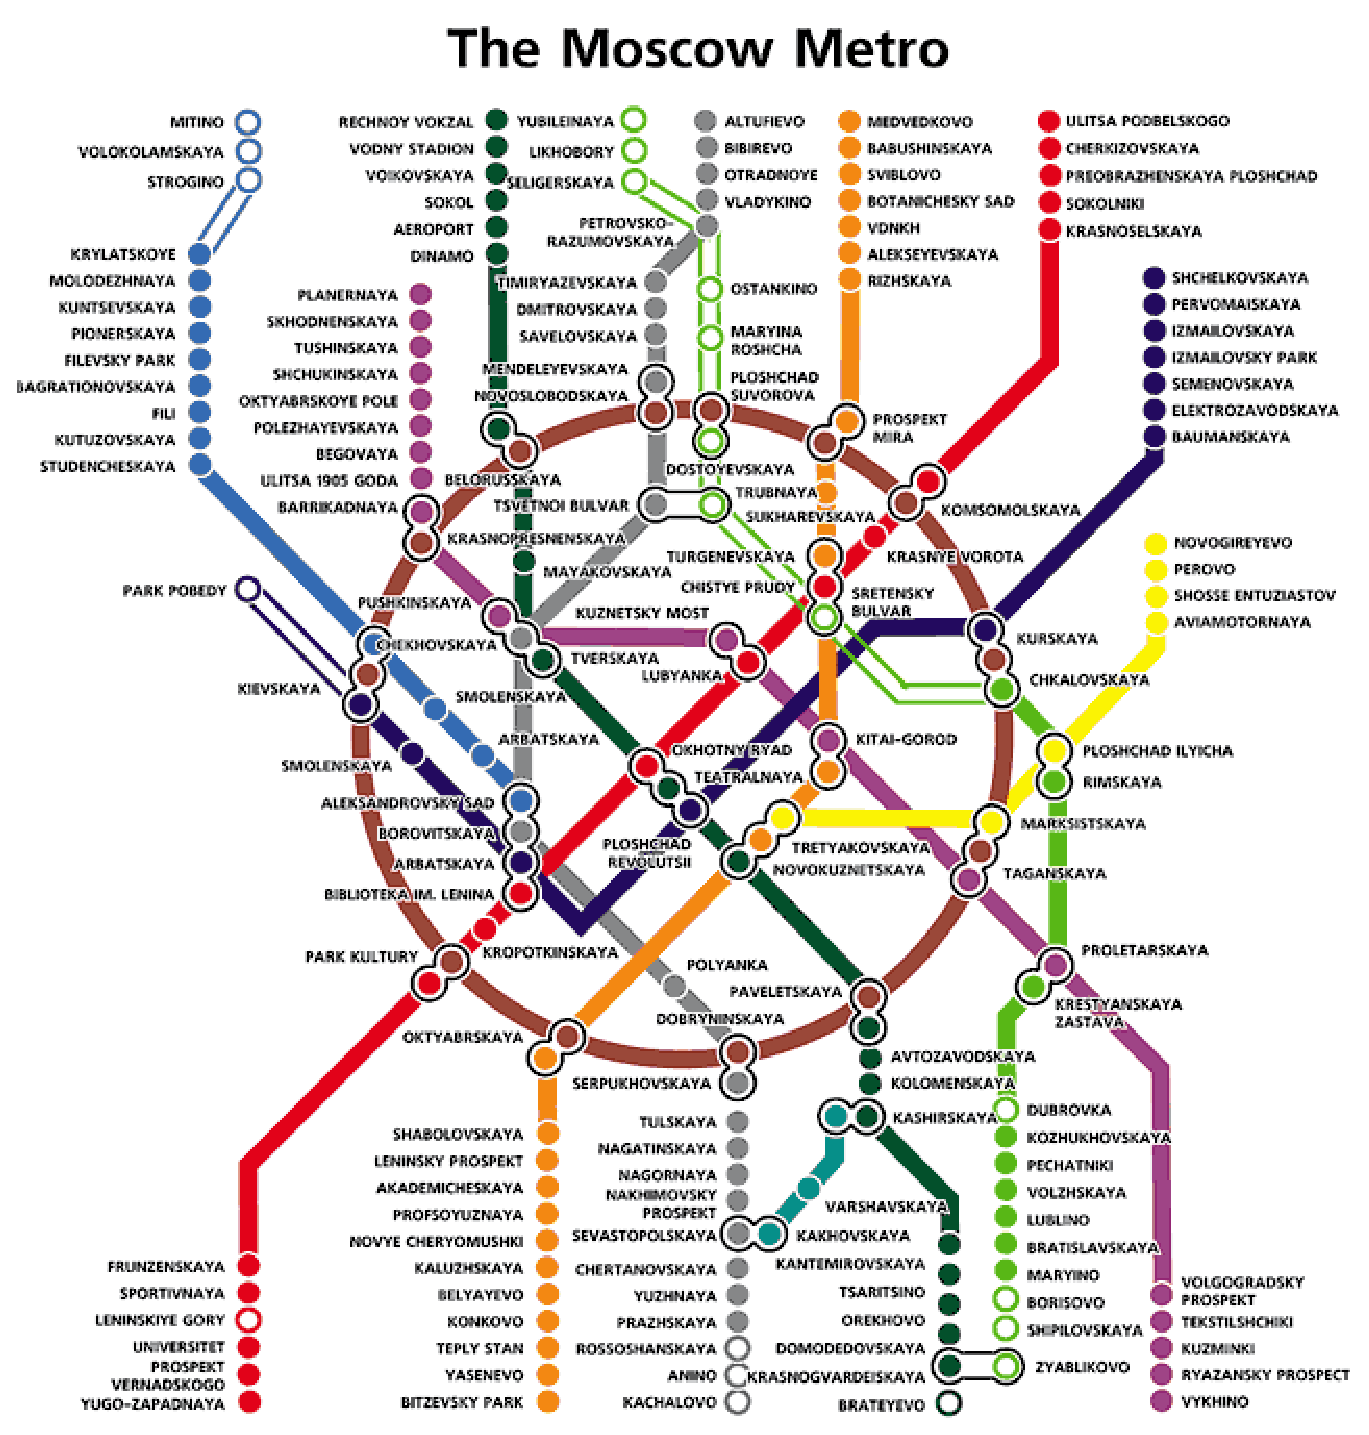
\includegraphics[width=8cm]{Pics/subway_map}
\end{center}
\caption[Example topological map.]{An example of a topological map, the Moscow subway map.}
\label{fig:subway}
\end{figure}

With a topological map, the robot is restricted to the routes along
the edges of the map. The robot cannot take shortcuts even if they are
physically possible. 

%\NOTE{cite topological papers}

Metric maps are generally more detailed and hence useful. 
The robot pose and the map features are defined in a single
reference frame. Metric maps can have landmarks (unique or identical),
or they can represent the environment as an occupancy grid. Each cell
of an occupancy grid map is assigned a probability value of being
``occupied by an obstacle''. A hybrid metric map, that combines
landmarks and occupancy grids has also been proposed in
\cite{guivant04}.  

%%% The most common approach to Simultaneous Localisation and Mapping
%%% (SLAM) is based on Extended Kalman Filter
%%% \cite{ekf_slam,dissanayake01}. A more recent development is FastSLAM
%%% \cite{fastslam,nieto2003} and a continuation of this work
%%% FastSLAM 2.0 \cite{fastslam2}.


\section{Localisation} 
\label{sec:Localisation}

%What is localisation
%Typically the robot
%uses a collection of sensors to collect observations of the 
%Why does the robot need to localise
%Topological vs Metric
%Subclasses of the localisation problem

Robot localisation, estimating the pose of a robot, is one of the
fundamental problems in the field of mobile robotics. It is considered
one of the prerequisites for providing autonomous capabilities for a
mobile robot \cite{Cox91}.  The localisation algorithm can face three
possible problems

\begin{itemize}
\item {\bf Position tracking}\\
      The robot's initial pose is known with relatively high
      certainty. The robot keeps track of its pose as it moves through a
      familiar environment.

\item {\bf Global Localisation}\\ 
      The initial pose of the robot is unknown, or is given by a
      probability distribution $p(\x{0}{}{})$ with high variance. As
      the robot moves through the environment and collects
      observations, it determines its pose.

\item {\bf Kidnapped robot}\\ 
The robot is moving through the environment and is reasonably certain
about its pose. Suddenly it gets moved by an external force (think of
a robotic vacuum cleaner) to some other place within a known map. The
robot should be able to detect that its estimate of the pose is no
longer correct and re-localise.
\end{itemize}

Much research has previously concentrated on position tracking - in
fact many existing algorithms address only the first problem (see
review in \cite{Borenstein96}). Global localisation and the Kidnapped
robot problems have been addressed using multi-hypothesis Kalman
filters \cite{JensfeltKristensen01,Cox94}, Markov localisation
\cite{Fox99}, and Monte Carlo methods \cite{Thrun00j}.


\subsection{Problem Definition}

The problem of localisation can be thought of as a problem of
estimating the probability density distribution of robot pose
conditioned on the observation and control data.  This posterior is
typically called {\it Belief} and is denoted
\begin{equation}
  Bel(\x{k}{}{}) = p(\x{k}{}{} | \Uall{k-1}{}, \Zall{k}{}),
\label{eqn:localise_belief}
\end{equation}
where \Uall{k-1}{} is a set of all control inputs up to time $k-1$, and
\Zall{k}{} is a set of all observations up to time $k$. It is usually
desired to approximate the posterior recursively, otherwise one would
run into computation problems very quickly.  If we make a Markov
assumption that future data is independent of past data given the
robot pose, we have

\begin{eqnarray}
 p(\z{k} | \Zall{k-1}{}, \Uall{k-1}{})    &=& p(\z{k} | \x{k}{}{}) \\
 p(\x{k}{}{} | \Zall{k-1}{}, \Uall{k-1}{})&=& p(\x{k}{}{} | \x{k-1}{}{}, \U{k-1}{}).
\end{eqnarray}

We can transform \refEquation{eqn:localise_belief} into a recursive
formula by applying Bayes' rule (see \cite{Thrun00j} for a derivation)

\begin{equation}
Bel(\x{k}{}{}) = \eta p(\z{k} | \x{k}{}{}) \int 
                     p(\x{k}{}{} | \x{k-1}{}{}, \U{k-1}{}) 
                     Bel(\x{k-1}{}{}) d \x{k-1}{}{},
\label{eqn:localise_recursion}
\end{equation}

where $\eta$ is a normalisation constant. To implement the recursive
rule in \refEquation{eqn:localise_recursion} one needs to know the
distributions $p(\z{k} | \x{k}{}{})$ and $p(\x{k}{}{} | \x{k-1}{}{},
\U{k-1}{})$. These distributions are generally referred to as {\it
observation} (or sometimes {\it perception}) and {\it motion} models,
respectively. 

The motion model reflects the uncertainty in robot dynamics, so it is
generally independent of time $k$. The observation model is a function
of robot sensors and of the environment. If sensor characteristics do
not change with time and if features in the map are static (a common
assumption), the same observation model can be used for every time
step.

\subsection{Common Approaches to Metric Localisation}

%EKF
Several approaches to localisation have been proposed. One family of
algorithms use the Extended Kalman Filter\cite{Jensfelt99}. Approaches
based on the EKF linearise motion and observation models and
approximate the posterior distribution with a Gaussian. While being
computationally efficient, EKF based approaches have some
limitations. They are not capable of global localisation, hence the
initial pose of the robot should be known with relatively high
confidence. An EKF is only capable of representing a uni-modal
posterior distribution, meaning that in an ambiguous situation only
one of the position hypotheses can be considered. This can lead to
localisation failure if the wrong choice is made.

A mixture of Gaussians model can be used to allow for multiple
hypotheses \cite{JensfeltKristensen01,Cox94}, but the problems arising
from linearisation are still present in these approaches.

%Markov
Markov localisation uses a grid to model the posterior distribution
\cite{Fox99}. This approach is capable of global localisation, and can
deal with the kidnapped robot problem as well. Fox \etal\ \cite{fb99}
have shown that Markov localisation works well, even in highly crowded
environments. The main advantage of this approach is the ability to
model any complex distribution. This makes the algorithm more robust
and allows for global localisation. Drawbacks include finite grid
size, computational demands and the need for a complex implementation
to optimise the observation update and increase resolution ``on the
fly''.

%PF
Particle filter localisation (also known as Monte Carlo localisation)
algorithms model the posterior distributions as a set of particles
\cite{Thrun00j, JensfeltAustinWijk00b}. A particle filter is capable of
approximating any probability distribution, including multi-modal
distributions. It can perform global localisation and can be used to
solve the kidnapped robot problem. Unlike grid-based algorithms,
particle filters have a floating point resolution for robot pose, and so
can give a more accurate pose estimate. Although it is computationally
more demanding than EKF approaches, the increased robustness of this
algorithm makes it worth the additional computational resources. The
computational complexity of the particle filtering algorithm is $O(N)$
in the number of particles used to represent the robot pose. Increasing
the number of particles will result in greater accuracy and
robustness. It is therefore straightforward to trade off the
computational resources against performance.

\section{Simultaneous Localisation and Mapping}
\label{sec:SLAM}

\subsection{SLAM Problem}

This section introduces the problem of Simultaneous Localisation and
Mapping. %TODO: expand some refs

A robot starts at time 0 at location \x{0}{}{}, executes a series of
motion commands $\Uall{k}{} = [\U{0},\U{1}...\U{k}]$ and collects a
set of observations at every step
$\Zall{k}{}=[\z{0},\z{1}...\z{k}]$. In practice observation and motion
commands are not synchronised, however this can be easily accommodated
in the implementation. It is therefore commonly assumed that
observation and motion happen at the same discrete time interval.
Control and perception of the robot are subject to noise.

%%% NOTE: above sentence might go

\SILENT{$[\mape{}{}{1},\mape{}{}{2}...\mape{}{}{n}]$}

SLAM seeks to find the true path of the robot up to time $k$,
$\Xall{k}{}{} = [\x{0}{}{}, \x{1}{}{}, ... \x{k}{}{}]$, and the true
model of the environment, $\map{k}{}{}$. Since there is an inherent
uncertainty in the robot's observation and motion, one generally
cannot give an exact description of the robot's path and a map of the
environment. However, it is possible to construct a probabilistic
model that assigns a likelihood to every path-map combination given
all the available observations, control inputs and the initial pose of
the robot:

\begin{equation}
 p(\Xall{k}{}{}, \map{k}{}{} | \Zall{k}{}, \Uall{k}{}, \x{0}{}{}).
\label{eqn:map}
\end{equation}

Assuming that odometry errors are independent of the observation
errors and of the environment model, one can separate the model into
an observation and motion parts and define:

\begin{enumerate}

\item The model of the robot's motion $P(\x{k}{}{} | \Uall{k}{})$. \\
If one makes a further assumption that past odometry errors have no
effect on future errors, one can represent robot motion as a Markov
process, with probability distribution 
\begin{equation}
 P(\x{k}{}{} | \Uall{k}{}) \equiv p(\x{k}{}{}| \x{k-1}{}{}, \U{k})
\end{equation}


\item The model of the robot's perception
$p(\z{k}| \x{k}{}{},\map{k}{}{}, \Zall{k}{})$.\\
Here again an assumption is made that errors in the measurements are
independent of past errors, hence

\begin{equation}
p(\z{k}| \x{k}{}{},\map{k}{}{}, \Zall{k}{}) \equiv 
  p(\z{k}| \x{k}{}{},\map{k}{}{})
\end{equation}

\SILENT{
\item The data association model (depends on the environment and the sensor)
\begin{eqnarray}
 p(\z{k} \equiv noise), \\
 p(\z{k} \equiv new | \x{k}{}{}, \map{k}{}{}),\\
 p(\z{k} \equiv \mape{}{}{\asc{k}} | \x{k}{}{}, \map{k}{}{}).
\end{eqnarray}
}

\end{enumerate}

Equipped with the knowledge of these distributions one can in
principle compute the exact posterior by considering every possible
path, map and data association decision combination. In practice,
however, computing such a distribution exactly is not possible due to
the high dimensionality of the system. Reasonably good approximations
can, however be obtained, and can be computed incrementally in
real-time.

The two most common approaches to solving the SLAM problem are the EKF
based algorithm \cite{ekf_slam} and a particle filter algorithm called
``FastSLAM'' \cite{fastslam}.

\subsection{Kalman Filter Approach}
The Extended Kalman Filter approach treats the SLAM problem as a state
estimation problem in which the state consists of the robot pose and
locations of all landmarks. Usually the number of features is not
known in advance, so most implementations have some provision for
adding new elements to the map as new observations are obtained. EKF
SLAM requires linearisation of the robot's motion and perception
models, so that the estimation error can be modelled by a Gaussian
distribution.  The computation complexity of the algorithm is
$O(K^2)$, where $K$ is the number of features in the map
\cite{ekf_slam}.

Considerable research has addressed the computational performance of
the EKF approach to SLAM \cite{williams:acra2001, williams2001esa,
  knight2001tct, guivant01, tim_bailey, uhlmann97nondivergent,
  tardos02:_mappin_local_indoor_envir_using_sonar_data}.  It is
possible to exploit the fact that only a small subset of the whole map
is observed at any given time to reduce the computational burden.
Compressed EKF \cite{williams:acra2001} is an optimal approach that
reduces the computational cost of measurement update to $O(K_a^2)$,
where $K_a$ is a number of features in the local region of the global
map.  This approach still requires a costly $O(K^2)$ global
registration stage when robot changes from one local region to the
next. A sub-optimal version of the same algorithm bounds the cost of the
global registration stage.


The most important limitation of the EKF approach is the inability to
model multiple data association decisions. Every observation has to be
classified as noise, a new feature or an observation of an existing
feature.  It is possible to postpone the final decision by running
multiple Kalman filters in parallel. Alternatively, one can try to
improve the quality of data association decisions. Batch data
association techniques like
\cite{neira01:_data_assoc_stoch_mappin_using,
tardos02:_mappin_local_indoor_envir_using_sonar_data} can reduce the
ambiguity of data association, but it is impossible to eliminate this
problem completely. It is impossible to undo incorrect data association
in EKF, as a result EKF is quite sensitive to data association
errors. Detecting large cycles is a very difficult problem for EKF SLAM,
due to the inability to deal with ambiguous data association.


\subsection{Particle Filter Approach}
FastSLAM uses particles to approximate the posterior distribution
\cite{fastslam}. Every particle maintains its own path, data
association decisions and the resulting map. The map is a collection
of independent landmarks. Particle locations are estimated using a
Kalman filters for every landmark. FastSLAM requires linearisation of
the perception model, but it samples directly from the motion model.
As a result, no change to the motion model is required. FastSLAM can
be implemented in $O(M\log K)$, where $M$ is the number of particles
and $K$ is the number of landmarks.

Given enough particles, FastSLAM produces a reasonable estimate of the
posterior distribution. Unfortunately it is not clear how many particles
are needed for a particular problem. A modified version of the FastSLAM
algorithm \cite{fastslam2} uses an alternative sampling technique to
generate particles where they are needed most, therefore reducing the
number of particles needed. The authors \cite{fastslam2}, demonstrate
that in some cases even one particle is enough.

The main advantage of FastSLAM is its ability to handle multiple data
association decisions \cite{Montemerlo2003}, which makes it a more
robust algorithm. From the implementation perspective, FastSLAM is
trivial to parallelise since computation per particle is independent
of other particles. This allows implementations to exploit the recent
trend towards larger numbers of processors, rather than faster
processors, in emerging computational hardware.

\subsection{Effect of Ambiguous Data Association on Posterior
  Distribution}
\label{sec:AmbiguousDA}

One of the advantages of the EKF - representing a posterior
distribution as a Gaussian, is also a weakness. Linearisation allows
for an efficient implementation and provides a sound mathematical
background for the algorithm. However, posterior distributions arising
in SLAM can be distinctly non-Gaussian depending on the environment,
robot dynamics and sensor characteristics.

One of the factors affecting the true posterior distribution is the
quality of data association decisions. In the case of perfect data
association, the posterior distribution tends to have a single peak
and can be approximated with a Gaussian quite well. When data
association is unreliable, multiple plausible hypothesis for data
association arise. These multiple hypothesis produce a multi-modal
posterior distribution.

\begin{figure}
\begin{center}
\subfigure[Experiment setup]{
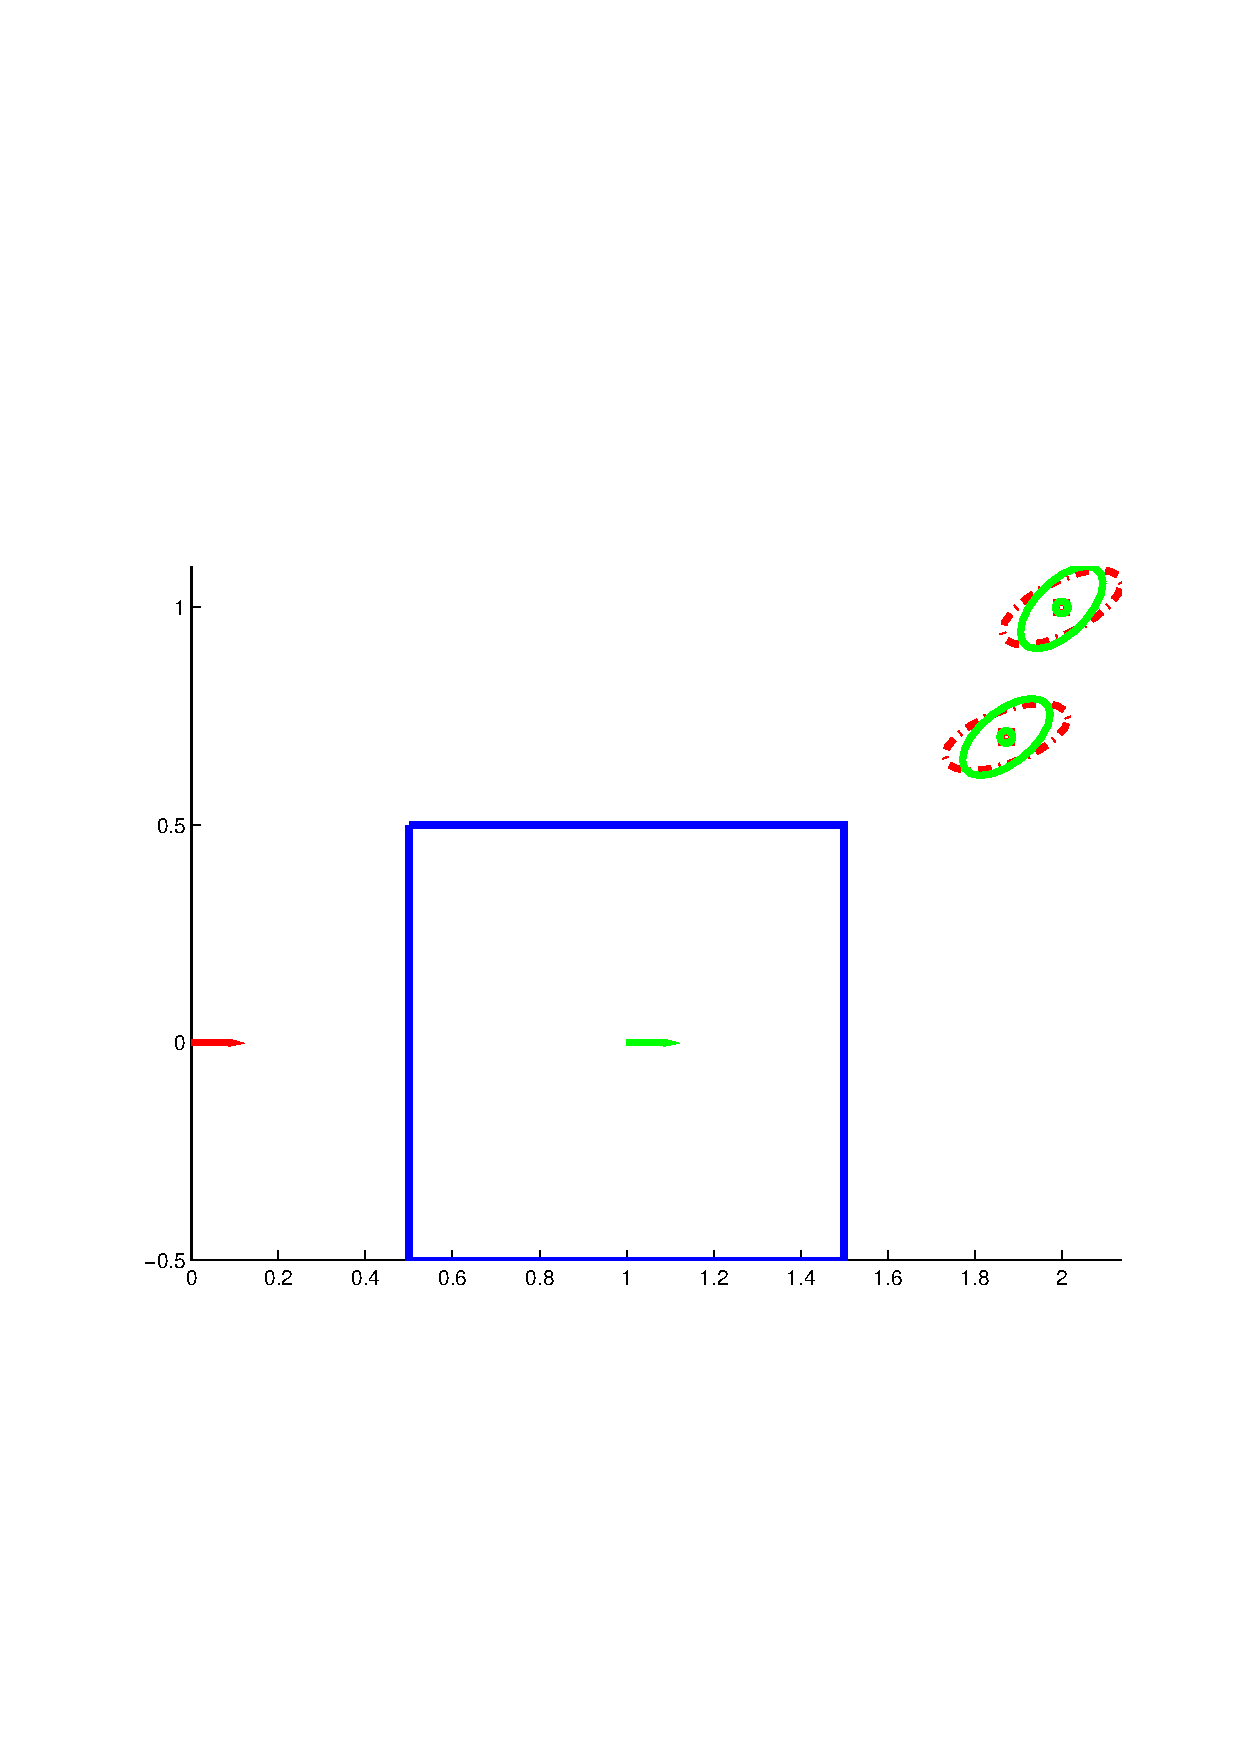
\includegraphics[width=6cm]{Pics/post_example}
\label{fig:post_example}
}
\subfigure[$p({\bf x} | {\bf u})$]{
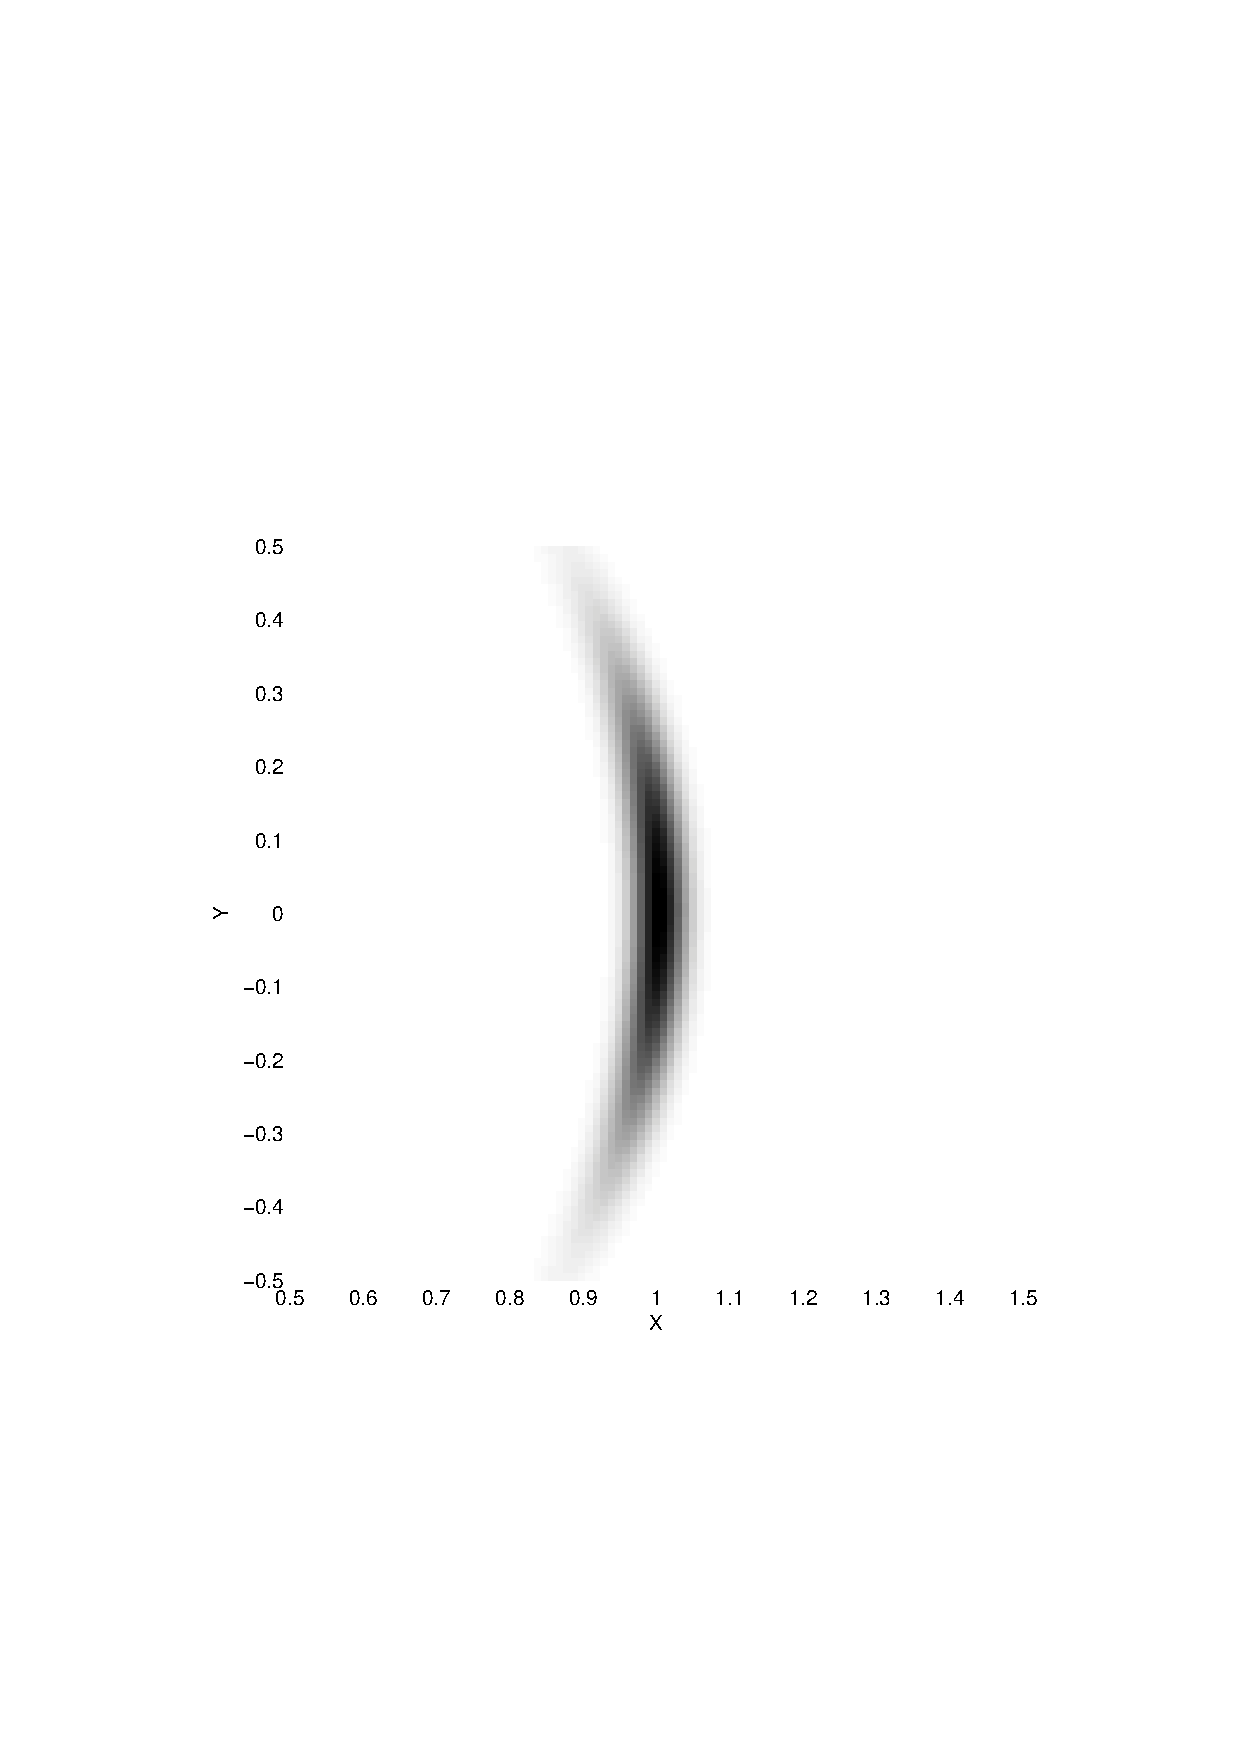
\includegraphics[width=6cm]{Pics/post_odo}
\label{fig:post_odo}
}\\
\subfigure[Known data association: $p({\bf x} | {\bf z})$ ]{
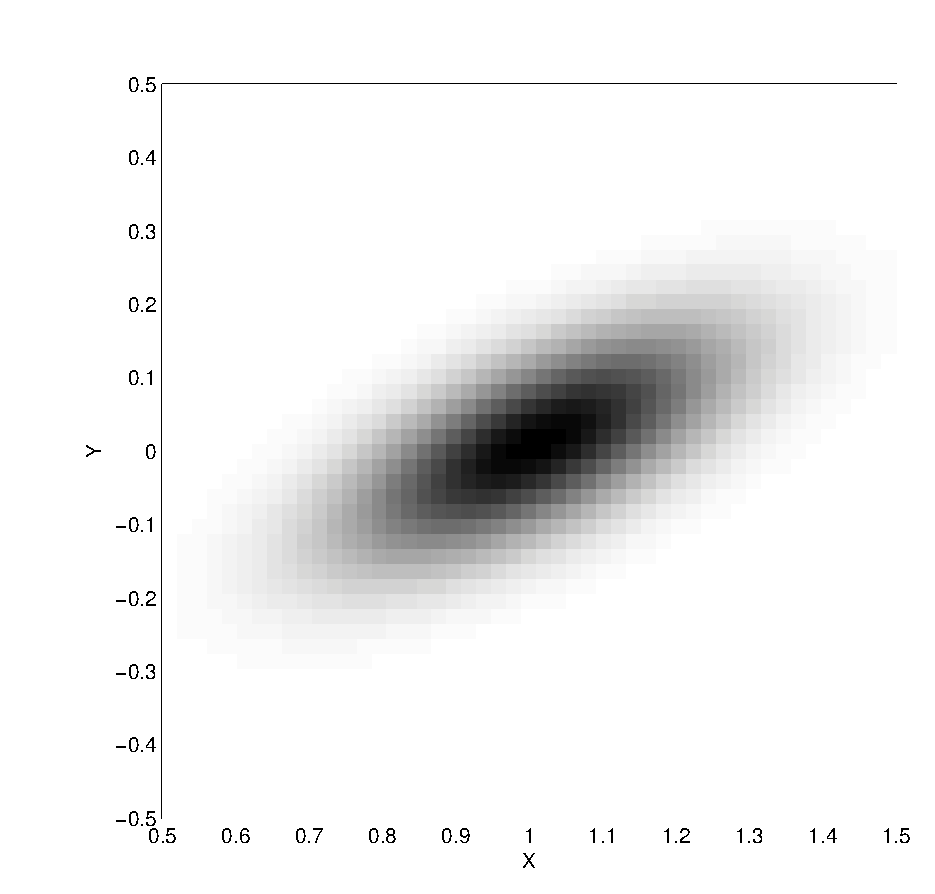
\includegraphics[width=6cm]{Pics/post_obs}
\label{fig:post_obs}
}\quad\space
\subfigure[Known data association: $p({\bf x} | {\bf u},{\bf z})$]{
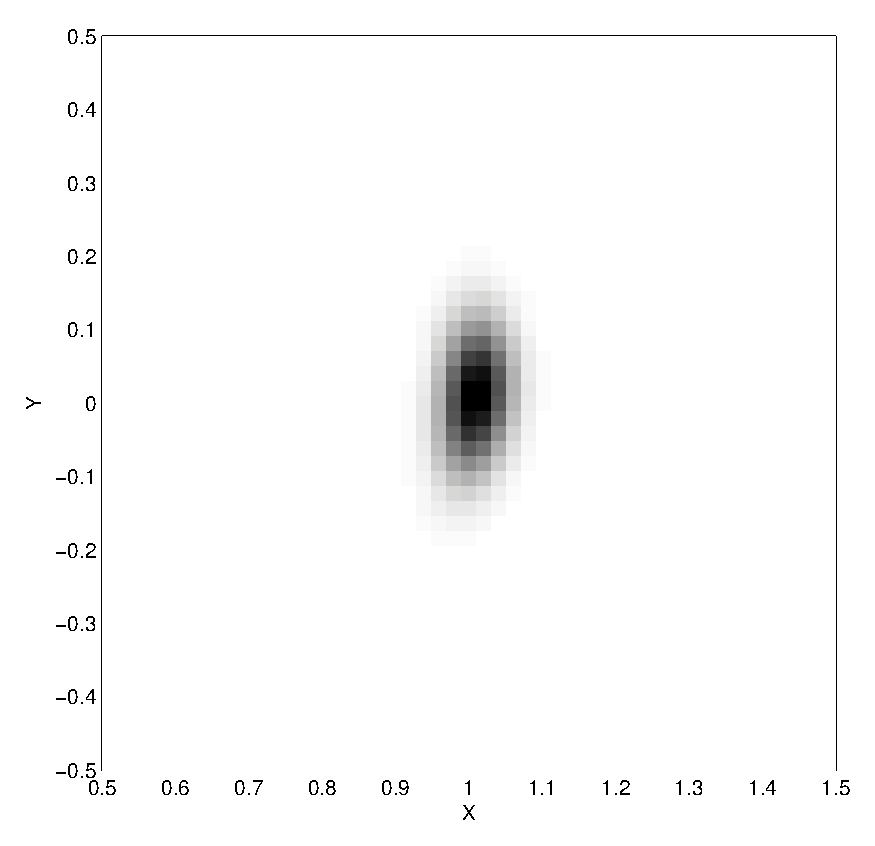
\includegraphics[width=6cm]{Pics/post_obsodo}
\label{fig:post_obsodo}
}\\
\subfigure[Ambiguous data association: $p({\bf x} | {\bf z})$ ]{
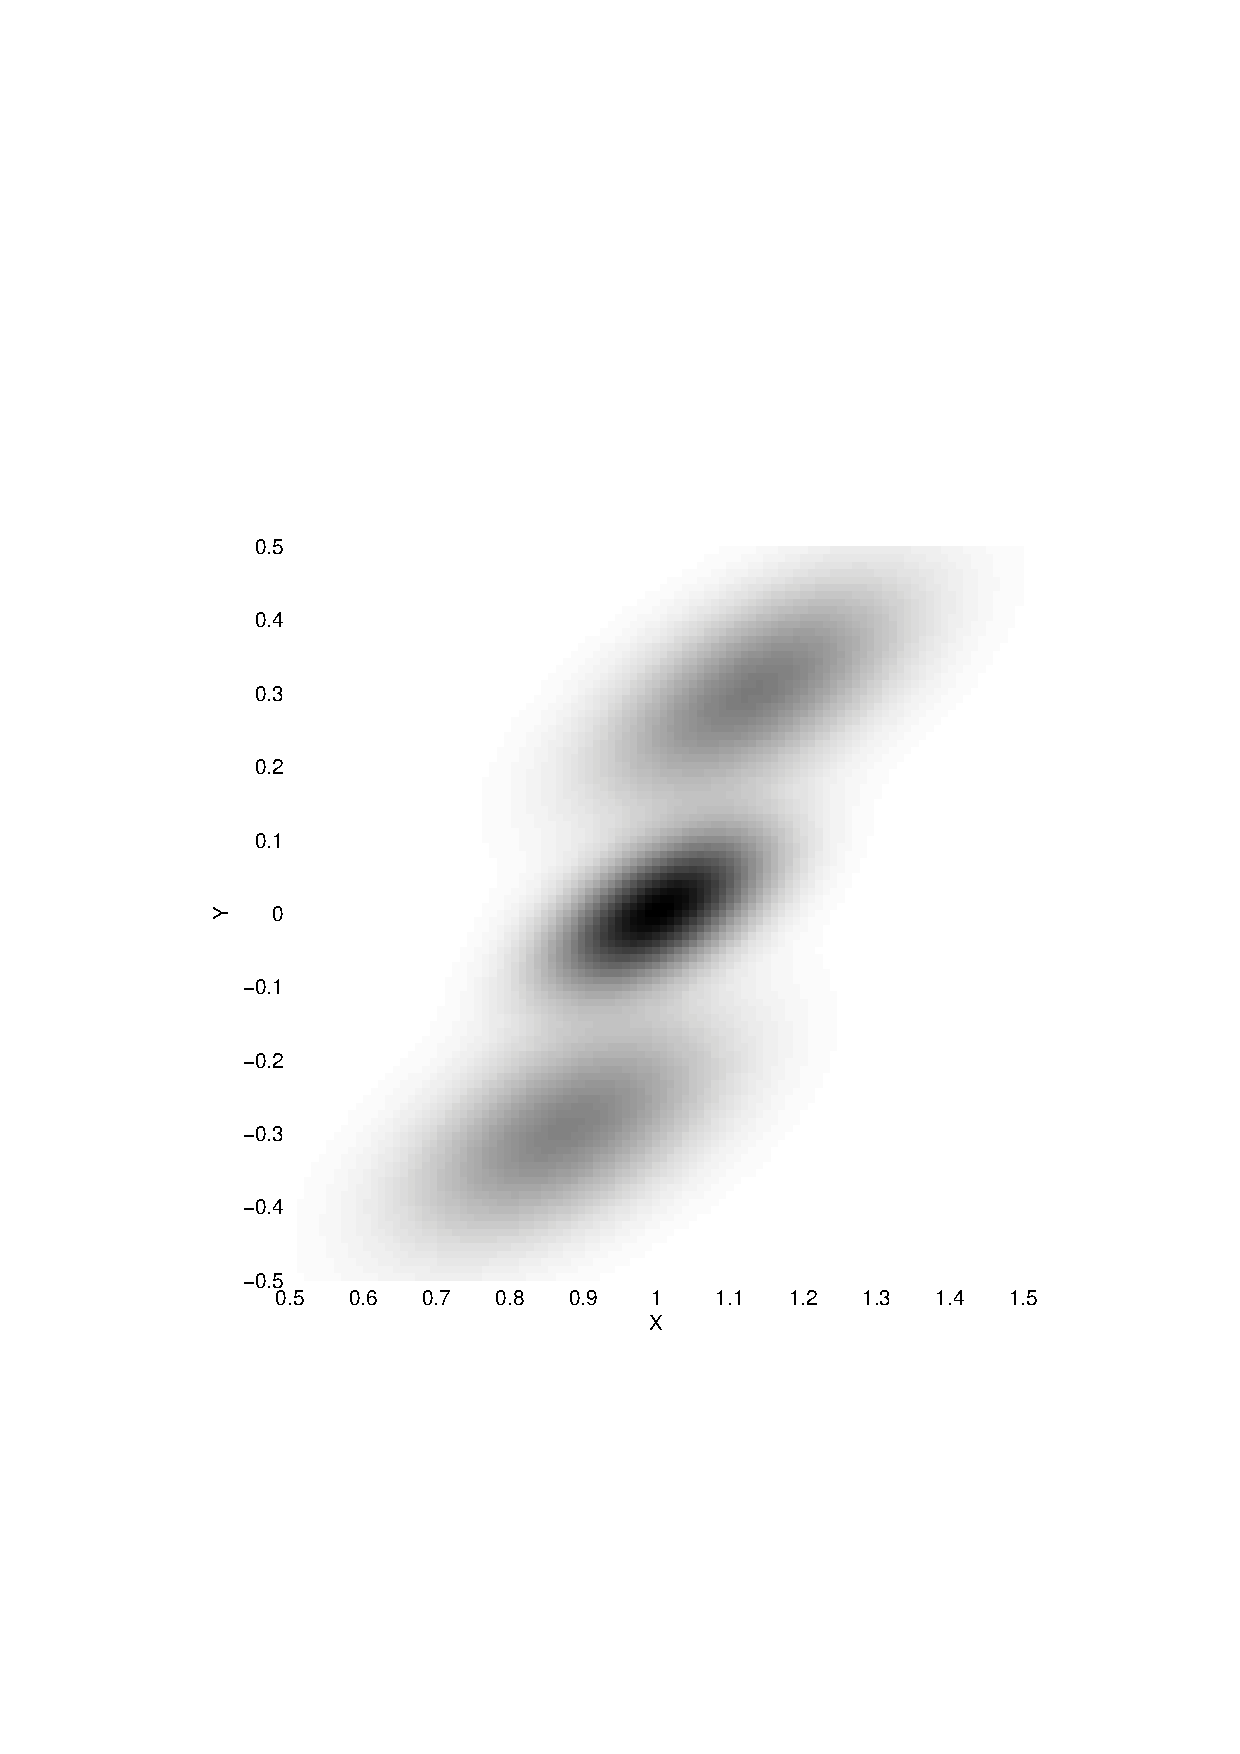
\includegraphics[width=6cm]{Pics/post_obs_}
\label{fig:post_obs_}
}\quad\space
\subfigure[Ambiguous data association: $p({\bf x} | {\bf u},{\bf z})$]{
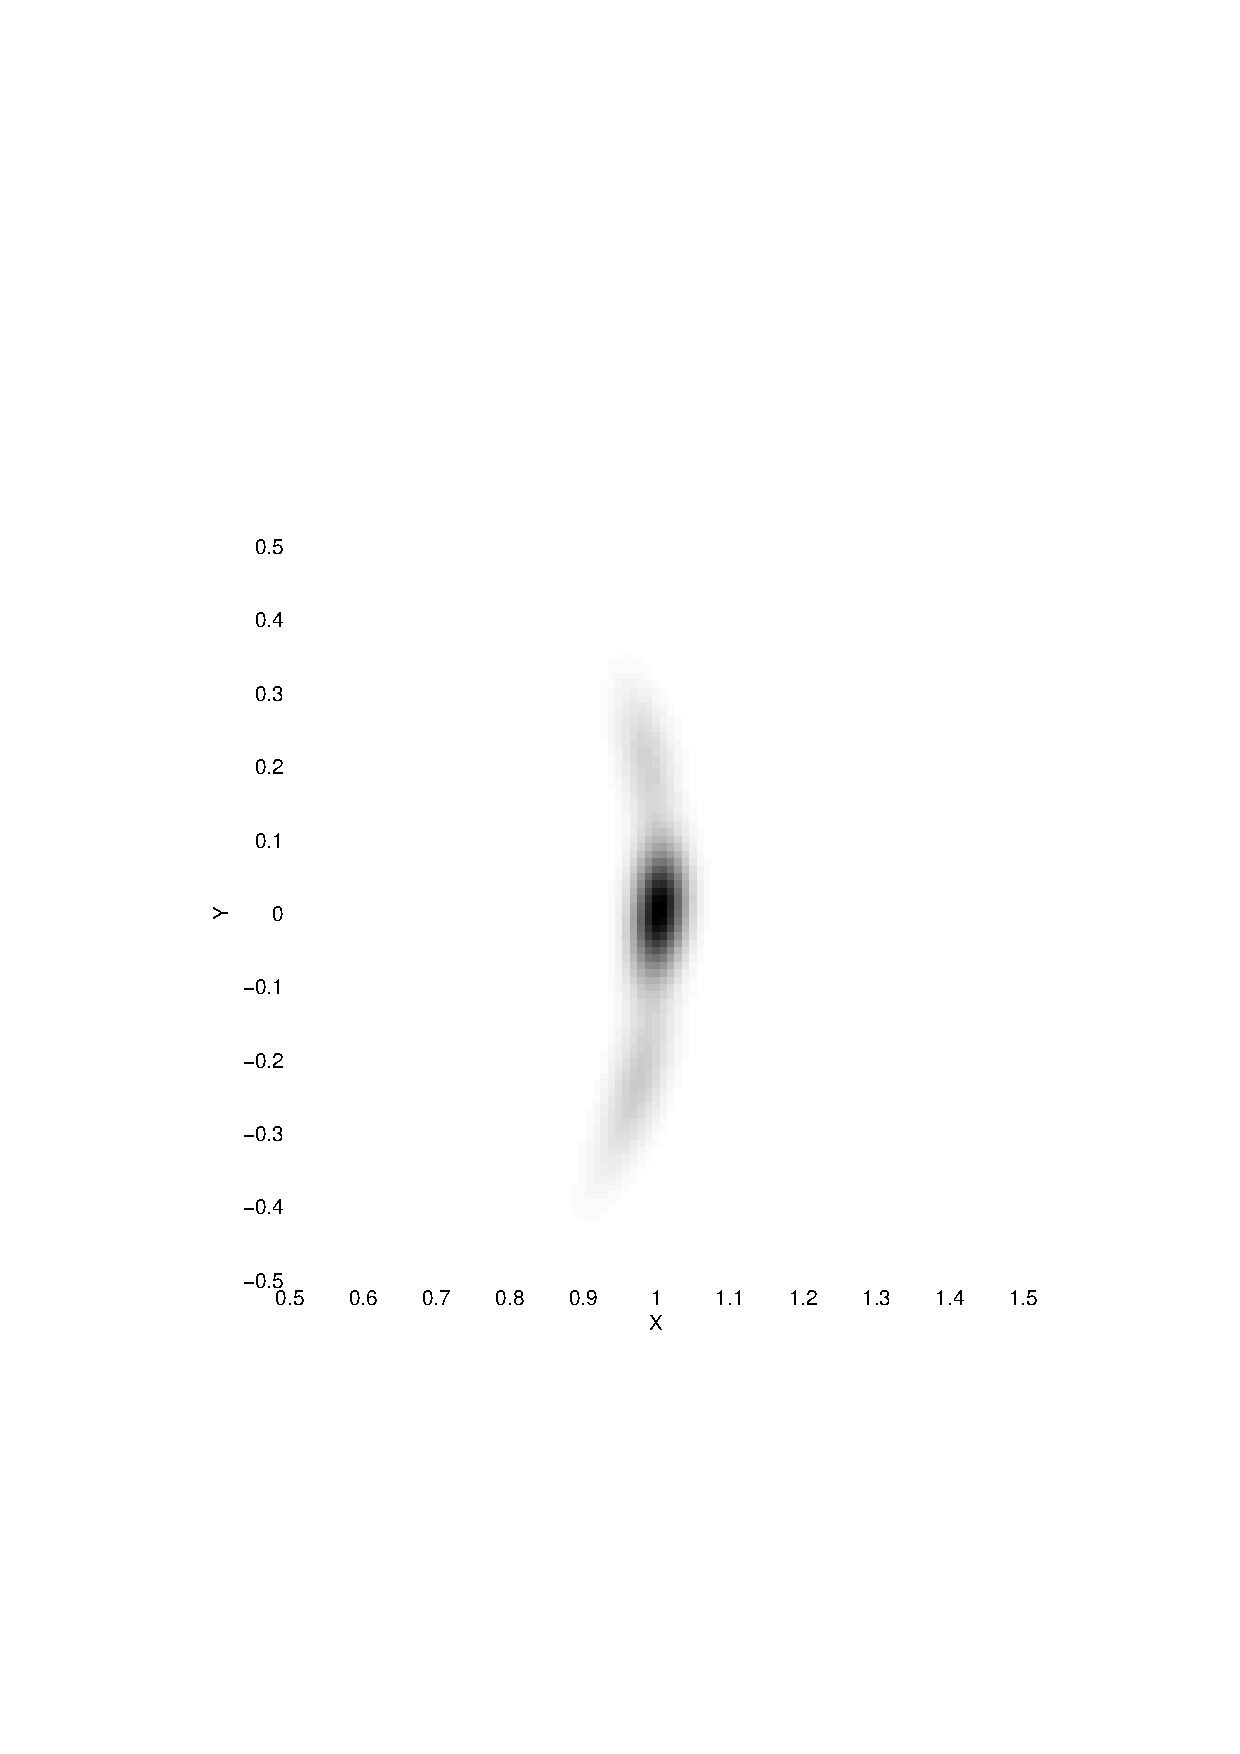
\includegraphics[width=6cm]{Pics/post_obsodo_}
\label{fig:post_obsodo_}
}
\end{center}
\caption[Robot pose uncertainty, example]{In \ref{fig:post_example} a
  robot makes an observation at point (0,0), then moves 1 meter
  forward and makes another observation. The square shows the region
  for which pose uncertainty is computed. The resulting uncertainty
  in robot pose just before the second measurement is shown in
  \ref{fig:post_odo}. Two scenarios are considered: known and
  ambiguous data association (rows two and three respectively).  The
  uncertainty due to the measurement is shown in \ref{fig:post_obs}
  and \ref{fig:post_obs_}. The robots pose uncertainty after
  incorporating the measurement is presented in \ref{fig:post_obsodo}
  and \ref{fig:post_obsodo_}.}\label{fig:post_all}
\end{figure}

To illustrate this point, consider a simple mapping example: the world
consists of two point landmarks and a robot living on a
two-dimensional plane, as shown in \refFigure{fig:post_all}. Robot
pose is defined by its location on the plane only, ignoring the
orientation of the robot (one can assume that the robot has an
extremely accurate compass). The robot is equipped with a sensor that
reports landmark location relative to the robot pose. The error of the
sensor is zero-mean Gaussian.

The robot makes an observation at point (0,0), then moves one meter
forward and makes another observation,
see \refFigure{fig:post_example}. The robot dynamics are controlled by
the following equation:
$$
  \Vector{x_k\\y_k} = \Vector{ x_{k-1} + r_k cos(\Theta_k)\\
                               y_{k-1} + r_k sin(\Theta_k) },
$$
here control inputs at time $k$ are $r_k$ and $\Theta_k$ for distance
and direction of travel, respectively. Gaussian noise in actuation
produces a banana-shaped distribution over the robot pose, shown in
\refFigure{fig:post_odo}.

Consider first the scenario when data association is perfect. After
execution of the motion command the robot observes the landmarks once
more. Since the observations were not certain for both first and
second observation, the pose estimate that can be derived from the
measurements has a significant uncertainty. This is illustrated in
\refFigure{fig:post_obs}. The posterior distribution is non-Gaussian
in this case as well, although the difference is not as apparent as in
the motion example. The posterior distribution of the robot pose given
observations and control input is shown in
\refFigure{fig:post_obsodo}, while it is not strictly Gaussian, it can
be argued that it can be approximated by a Gaussian reasonably well.

In the case when data association is ambiguous, the posterior
distribution is slightly more complicated. Lets assume the robot has
three equally likely data association hypotheses. 

\begin{itemize}
\item Observations 1 and 2 map to landmarks {\bf a},{\bf b}
\item Observation 1 maps to landmark {\bf b}, observation 2 is spurious
\item Observation 2 maps to landmark {\bf a}, observation 1 is spurious
\end{itemize}

Each of these hypotheses by itself produces an almost Gaussian
posterior distribution, but when combined the result is a multi-modal
distribution shown in \refFigure{fig:post_obs_}. The posterior
distribution of the robot pose given observations and control input is
then as shown in \refFigure{fig:post_obsodo_}. Clearly this
distribution differs significantly from a Gaussian.

The example presented shows that non-Gaussian distributions in robot
posterior can arise as a result of an ambiguous data
association. Approaches to SLAM that can deal with such distributions
therefore might have an advantage in such situations.


\section{Loop Closing}
\label{sec:back_loop}
%Problem definition
  % Detect
  % Correct

The problem of loop closing arises when mapping a large cyclic
environment. When the robot returns to a previously mapped region via
a large loop, rather than by back-tracing its own steps, it needs to
recognise the place as previously mapped. Failure to do so will result
in inconsistent map.  As the robot moves through an unexplored
environment while building the map, it becomes more and more uncertain
about its pose relative to the regions it mapped in the past.
Increased uncertainty in robot pose makes it more difficult to
detect a place the robot has already mapped.

%The increase in the uncertainty makes it hard for the robot to detect when it comes
%back to the region it has mapped already. 
%Failure to detect revisiting results in an inconsistent map.

In order to build a consistent map, the robot needs to be able to
detect the places it has visited to before and correct its estimate of
the path along the loop. The problem of mapping large cyclic
environments has been addressed by several researchers.


%what is there now
  %Lu Milios (scan matching + optimisation)
  %Gutman   (scan matching + confirm + handles high uncertainty)
  %Thrun's  (EM)
  %Fergusson (EKF mines)
  %Atlas


Lu and Milios \cite{lu97:_global} propose an algorithm they call
``consistent pose estimation''. The algorithm uses laser scan matching
and linearised global optimisation over scan poses to build a scan map
of the environment in a single global frame. The approach builds a
network of robot poses at which a laser scan has been taken. The poses
are connected by ``weak'' and ``strong'' links. The links represent
the spatial relations between poses. Weak links are derived from
odometry and strong links are derived from the scan matches. The
algorithm then finds a global configuration of the poses of the places
by minimising a cost function. If one thinks of links as springs, the
algorithm finds the configuration that reduces the sum of forces
exerted by the springs. Spatial relations are modelled by Gaussians,
and the cost function is the sum of the Mahalanobis distances.

The method by Lu and Milios is very sensitive to the initial estimate
of the robot pose just before loop closing. Since the pose estimate is
derived from local scan matching and odometry, it can, in principle,
have unbounded error. If the initial estimate is too far from the true
robot pose, the algorithm tends to converge to spurious local minima.
The method also has high computational complexity, $O(N^3)$ in the number of poses.

Konolige and Gutman
\cite{konolige99:_increm_mappin_large_cyclic_envir} provide a method
based on the ideas of Lu and Milios, but try to address these
problems. Instead of using single laser scan to find relations between
places they use a map correlation technique \cite{konolige99}. This
makes the system more robust to false correspondences. After detecting
loop closing, the algorithm runs consistent pose estimation. 

An interesting scan matching based mapping technique has been
developed by by Ferguson \etal\ \cite{fergusson2003}. In this
approach loop closing can be undone if the observations further down
the track do not support it.

Thrun \etal \cite{slam_thrun98b,Thrun98a,thrun98:_probab} suggest an
approach that uses an Expectation Maximisation (EM) algorithm to
construct maps of cyclic environments. The algorithm is given a
relatively small set of observations of sparsely positioned non-unique
landmarks and the set of all control inputs. In the expectation step the
algorithm computes the most likely robot path given the map and the
data. In the maximisation step the most likely map is computed given
the robots path from the E-step. The Expectation and Maximisation
steps are repeated until the map converges to the maximum likelihood
solution. This algorithm cannot be implemented in real-time because
it needs to have access to all of the future and past data to
determine the robot pose at any given time. %% check maximum likelihood

All of the methods presented so far build a map of the whole
environment in a single global reference frame. Recently, Bosse \etal\
\cite{bosse03atlas} suggest a mapping approach, \Atlas, that does not
require a global reference frame. The map structure used in this
approach is a hybrid topological/metric map.  Each node is a local map
and every link in the topological map represents a spatial
relationship between the two places it connects. 

\Atlas\ uses a combination of map matching and uncertainty projection
to detect when the robot re-enters a previously explored area.
Uncertainty projection computes the relative poses between the two
non-adjacent local maps. If according to this estimate, the two maps
might be overlapping, \Atlas\ tries to find the landmark
correspondences between the two maps. If the two maps match, the new
link is added to the topological map. The pose relation for this link
is computed from the landmark correspondences. In order to decrease
the probability of incorrect data association, \Atlas\ runs several
hypotheses at any given time. If, after closing the loop, the
observations do not match the map well enough, the loop closing
hypothesis will be discarded in favour of the new map hypothesis.


\section{Limitations of Metric Approaches to Mapping}

%Until recently there were two main strategies for map representations
%in robotics: topological and metric. 
%Problems with global mapping.
%Building an accurate metric map is not a trivial matter. 

While there exist several good methods for building metric maps, they
do not scale up to big environments. The main restricting factors are:

\begin{enumerate}
 \item Increase in the computational complexity. The larger the
  environment the longer it takes to execute an update with every new
  measurement.

 \item Increase of the robot pose uncertainty. As you run the
 algorithm for longer, errors tend to accumulate, especially in large
 environments. No matter how accurate your mapping process is,
 there is still going to be some residual uncertainty, and it will
 accumulate as the robot travels longer distance. The effect of such approximation
 errors is especially harmful when cycles are present.

 \item Increasing approximation error in the mapping procedure.

\end{enumerate}

The first point is fairly obvious: more landmarks require more
computation and more memory. Since the environment is considered as a
whole, one needs access to all landmarks to continue mapping. This
problem was tackled by Williams \etal\ using Constrained Local Submap
Filters \cite{williams:acra2001}. Their approach uses local maps for
building the immediate environment around the robot, effectively
forgetting about the rest of the world. The local map is then merged
into the global reference frame. This keeps the computational
requirements relatively constant, irrespective of the environment
size. The underlying mapping algorithm used in this approach is EKF
SLAM.

Increasing uncertainty is another fundamental problem when a map is
built incrementally, i.e. new measurements are added to the existing
map as they arrive. In order to add a measurement the robot needs to
solve a data association problem: is this observation from one of the
features already in the map, is it new or is it noise?  As the robot's
pose uncertainty in the existing map increases, data association
becomes more difficult. An incorrect data association decision becomes
more likely, leading to inconsistent maps. Even in the case when
perfect data association is possible (when unique landmarks are used),
increasing pose uncertainty will cause problems, since pose
uncertainty also means map uncertainty. Even if the robot manages to
re-localise itself, correcting the map can be a problem.

The problem of data association under uncertainty has been addressed
by \cite{neira01:_data_assoc_stoch_mappin_using,
  tardos02:_mappin_local_indoor_envir_using_sonar_data}.  Rather than
finding the mapping of a single observation to a landmark, these
approaches consider a set of observations simultaneously. While such
approaches make data association more robust to sensor pose
uncertainty, they do not completely resolve the problem of {\it
  increasing} uncertainty.


Algorithms that work on all of the data at once, like Expectation
Maximisation \cite{thrun98:_probab}, are not affected by this problem,
but their computational requirements are huge and they cannot operate
in real time, since all of the data has to be processed at once.

In the case of FastSLAM, data association is solved on a per particle
basis. Data association is therefore not affected by the increasing
uncertainty. FastSLAM can also correct the map after loop closing
automatically and in real time, by simply keeping only the ``good''
particles. Nevertheless the increasing uncertainty is still a
problem. In order to perform reliably, FastSLAM will require more and
more particles to accurately represent the increasing robot pose
uncertainty. Like any particle filtering algorithm, FastSLAM is
affected by the particle depletion problem: if there are not enough
particles in the right region, the algorithm will fail to detect a
loop-closing.

EKF SLAM tends to underestimate robot pose uncertainty, and as a
result it might fail to detect loop closing. Correcting the map and
the path, even if the robot does re-localise itself, is also a big
problem for EKF SLAM, and does require substantial computational
resources.

Another important limitation comes from the approximation error. Every
mapping algorithm is trying to compute the map as a joint posterior
distribution of robot poses and a map given all the observations and
control inputs. Since computing such a distribution in its true form
is rather impractical, all existing approaches try to approximate it.
As the environment size increases the effect of approximation becomes
more significant.

%%% EKF SLAM linearises the motion and observation models. FastSLAM
%%% approximates the robot pose by the set of particles, and assumes a
%%% Gaussian observation model. EM based SLAM has to make some assumptions
%%% about the environment and the robot motion. 


\section{Hybrid Approaches to SLAM} 

If one segments the environment into a number of smaller regions, and
maps each region separately (build local maps), one can avoid the
problem of unbounded complexity and also reduce the effects of
approximation errors.

Hybrid topological/metric maps
\cite{fergusson2003,bosse03atlas,Thrun98a} allow for accurate local
positioning by virtue of the metric component, yet are easier to
construct since computational complexity per local map is bounded. It
is also easier to close large cycles since closing a cycle in such a
map is just a matter of adding a link between two places in the
topological structure of the map.

%%% Existing hybrid approaches can be grouped into three broad
%%% categories: mainly metric, mainly topological, and truly hybrid. 
%%% 

Some of the hybrid methods desire to build a global metric map
\cite{Thrun98a, slam_thrun98b}. These approaches use topological
structure as an intermediate step only. The environment is split into
local maps, each local map is explored separately, and all maps are
then merged into a large, global map. Merging can happen incrementally
or as a single post-processing step. Some optimisation steps might be
used to enforce consistency of the global map. The main advantage of
such methods is a more robust loop closing behaviour. This is due to
the fact that loop closing is performed based on map matching.

Other methods build topological maps with independent metric maps for
each node \cite{Cho01,Kuipers00}. Metric maps are built for every node of the
topological map as an after thought. The relationships between nodes
is purely topological. Metric information is only used inside the
local maps.

More recently a tighter coupling of metric and topological
information started to appear in robotic research. A hybrid mapping
approach called \Atlas\ by Bosse \etal\ \cite{bosse03atlas} incorporates
metric information into the topological structure of the map. Every
link in the topological structure stores the spatial relation between
the two nodes (local maps) as a stochastic variable. 

%%% \Atlas\ is described in more detail in the next section.


\subsection{Atlas}

\Atlas\ by Bosse \etal\ \cite{bosse03atlas} is a hybrid
topological/metric approach to SLAM. \Atlas\ models environment as a
set of local maps of bound size. There is no single global reference
frame, only local transformations between adjacent local maps are
maintained. Spatial relationships are approximated by a Gaussian,
derived from the residual robot pose uncertainty of the mapping
process used to build the local maps.

\Atlas\ supports various underlying mapping modules for building local
maps. The two mapping modules presented in \cite{bosse03atlas} were
based on EKF SLAM using line and point features extracted from either
laser or sonar range data.

The main advantage of \Atlas\ is the map structure it uses. Moving
away from the single reference frame allows the mapping of large
environments with huge cycles in real time. Even though there is no
global reference frame, it is still possible to compute the relative
poses of any two local maps with some certainty, hence it is possible
to project the robot pose estimate from one reference frame to any
other, along with the uncertainty.


When closing large cycles, \Atlas\ relies on place recognition
(map matching) and the robot pose estimate to detect a revisiting
event. If the two maps match, and the robot pose derived from the
match is likely, a new link can be added to the topological structure.
In order to avoid false positives, a loop closing hypothesis is first
tested by considering how well the observations match the map.

There are, however, some limitations to this approach. When, for
instance, the robot returns to a previously mapped region it gains new
knowledge about the relative positions of the local maps. The robot
can use this knowledge to update the links in the map. \Atlas\ does
not perform this update because of the computational requirements
involved, although the authors mention that such update can be performed
after the mapping is complete. \Atlas\ uses metrics to test loop
closing hypotheses. These metrics do not necessarily correspond to the
true likelihood, making it difficult to predict the behaviour of the
algorithm in a new environment.

\section{Summary}

The past few decades of mobile robotics research provide powerful
tools for mapping and localisation. Existing algorithms tend to be
limited to relatively small environments. The main limiting factors
are:

\begin{itemize}
\item The computational burden: as size of the environment grows, so do
  the computational requirements of existing algorithms.

\item The data association problem in the face of uncertainty: 
   in large environments the uncertainty of the landmarks far away
  from the origin is high. That makes it difficult to perform correct
  data association.

\end{itemize}

Various optimisation techniques and faster hardware can expand the
capabilities of existing algorithms, but to overcome these limitations
new map representations are required. In particular new ways to model
uncertainty should be explored.

% TODO: my contribution in a paragraph 1-2 sentences.
%TODO: many people worked on EKF, fewer on FastSLAM, no work on PF +
%hybrid map models. Need to explore new data structures, not just keep
%trying to patch up EKF approach.
%We therefore chose to use FastSLAM to perform local mapping tasks.

% Some recent research in
% this area include \cite{bosse03atlas,fergusson2003}.




\nocite{tim_bailey,
bosse03atlas,
fergusson2003
thrun00,
dissanayake01,
SOG-Slam01,
guivant02:_simul,
guivant02:_solvin,
thrun02:_robot_mappin,
 zunino01:_simul,
 JensfeltKristensen01,
 JensfeltWijkAustin00a,
 JensfeltAustinWijk00b,
 anguelov02,
 hahnel02:_map,
 burgard99:_exper,
 schulz01:_track_multip_movin_objec_mobil_robot,
 castellanos99:_spmap,
 castellanos01:_multis,
 dudek00:_robus_place_recog_local_appear_method,
 konolige99:_increm_mappin_large_cyclic_envir,
 lu97:_global,
 gutmann96:_amos,
 williams:icra2002,
 williams:acra2001,
 Zimmer96,
 slam_kuiper91,
 slam_kuipers88,
 Thrun00j,
 Fox99,
 Cox91,
 Borenstein96,
 kk2002,
 sidenbladh00stochastic,
 Cox94,
 Thrun02h,
 Bennewitz02a,
 Liu01a,
 Dellaert00c,
 nieto2003, 
 konolige99,
 doucetraoblackwellised,
 guivant04,
 newman03,
 vandermerwe00_tr,
 vandermerwe2000,
 wan01unscented,
 unscented,
 Margaret_hybrid_maps,
 kuipers1978,
 KuipersLevitt88,
 Kuipers00,
 Buzan04,
 uhlmann97nondivergent,
 julier97new,
 julier96general,
 julier99scaled,
 doucet98sequential,
 DA_Lazy,
 Kuipers2004,
 kk2004}



% LocalWords:  Sensorimotor Preoperational odometry EKF FastSLAM Kalman Siegel
% LocalWords:  Kuipers Golledge linearise Gaussians linearisation Milios
% LocalWords:  Mahalanobis minima Konolige Gutman Thrun Bosse Submap



\chapter{Background Theory and FastSLAM}
\label{chpt:Overview}
This chapter introduces background theory, in particular Kalman and
Particle filtering and the application of these techniques to the
problem of simultaneous localisation and mapping (SLAM). First a
notation that will be used throughout this document is introduced in
Section~\ref{sec:Notation}. Section~\ref{sec:Kalman} gives a brief
overview of Kalman filter and Extended Kalman (Section~\ref{sec:EKF}).
Particle filter is introduced in Section~\ref{sec:PF}. A comparison of
Particle filter vs EKF follows in Section~\ref{sec:PFvsEKF}. A brief
overview of Localisation is given in Section~\ref{sec:Localisation},
followed by an overview of SLAM in Section~\ref{sec:SLAM}. Finally a
problem of revisiting or ``loop closing'' is discussed in
Section~\ref{sec:back_loop}.


\section {Notation}
\label{sec:Notation}

The pose of the robot is represented by $\x{k}{}{a}$. Superscript $a$
indicates a reference frame, $k$ is a discrete time. A map of the
region $a$ at time $k$ is $\map{k}{}{a}$. In the case when we need to
differentiate between different particles, we add an extra superscript
$m$ to indicate a particle index $\x{k}{a}{m}$ and $\map{k}{a}{m}$. A
control input at time $k$ is $\U{k}$. An observation taken at time $k$
is $\z{k}$. Further notation will be introduced later on in this
thesis. \refTable{tab:notation} summarises most of the symbols used in
this thesis.



\SILENT{
This section describes the notation that will be used throughout the
rest of the document. We reserve letter $k$ to represent discrete
time, letter $t$ will represent continuous time. Letters $a$ and $b$
will be used to index map frames. Letter $m$ is used to represent
particle index, the $m$-th particle or belonging to the $m$-th
particle. Index $i$ is reserved for numbering elements of the finite
sets, that do not directly depend on time, for example the map is a
finite set of landmarks, that does not directly depend on time.

The discrete time index will be a subscript, for example \z{k}. The
element index $i$ will also be subscript, if both time and element
index are present, the time index will be followed by a comma followed
by the element index.

Map and particle indices will be superscripts, if both present, the
map index will be first, followed by a comma followed by the particle
index. For example \x{}{a}{m} means the $m$-th particle in the $a$-th
map. Table~\ref{tab:notation} describes variables we will be using in the
thesis and their meaning.
}

\begin{table}[ht]
\begin{tabular}{|l|l|}
\hline
%
\x{k}{a}{m} & pose of the $m$-th particle in the $a$-th map frame 
              at time $k$. \\
\Xall{k}{a}{m} & path of the $m$-th particle in the $a$-th map frame 
                 from time $0$ to time $k$. \\
%
\U{k}    & control input at time $k$.\\
\Uall{k}{a} & subset of all control inputs up to time $k$, that apply to the map frame $a$.\\
%
\z{k}    & observation at time $k$. \\ 
\Zall{k}{a} & subset of all observations up to time $k$, that apply to the map frame $a$. \\ 
%
\Teleport{k}    & teleportation at time $k$.\\
\TeleportAll{k}{a} & subset of all teleportations up to time $k$, that apply to the map frame $a$.\\
%
\map{k}{a}{m} & map of the $m$-th particle in the map frame $a$ at time $k$\\
\mape{a}{m}{i} & $i$-th map element from the $m$-th particle's map in 
                  the map frame $a$.\\
%
\s{k}{a}{m} & $m$-th particle in the SLAM particle filter at time $k$,
              in the map frame $a$.\\
\Sall{k}{}    & set of all particles in the SLAM particle filter at time $k$.\\
%
\tr{i}{a}{b} & transition vector from map frame $a$ to map frame $b$. \\
%
\Trall{a}{b} & a set of transition vectors from map frame $a$ to $b$.\\
%
%
\sample{a}{p(A)}& $a$ is a sample from the distribution $p(A)$.\\
\gpath{a}{b} & path from map $a$ to map $b$.\\
\hline

\end{tabular}
\caption{Notation used throughout the thesis.}
\label{tab:notation}
\end{table}


\section{Kalman Filter}
\label{sec:Kalman}
%A bit of history
R.E. Kalman published his famous paper describing a recursive solution
to the linear filtering problem in 1960 \cite{kalman60}. Since then
the Kalman filter has been the subject of extensive research and
application in various fields of science. It is used heavily in the
science of robotics for localisation and mapping purposes.  Kalman
filtering is used in this research. What follows in this section is a
brief introduction to Kalman filtering.

The Kalman filter addresses a general problem of estimating the state $
\x{k}{}{} \in \Rset^n$ of a discrete-time controlled process that is
governed by the linear stochastic difference equation
\begin{equation}
\x{k}{}{} = A_k \x{k-1}{}{} + B_k \U{k-1} + w_{k-1},
\label{eqn:kalman_process}
\end{equation}
where $A_k$ is a matrix that describes evolution of the state from
time $k-1$ to $k$ in the absence of control input or process
noise, matrix $B_k$ relates control input $\U{k-1} \in \Rset^l$, to
the change in the state vector and $w_k$ is a process noise.

Indirect measurement of the state $\z{} \in \Rset^m$ is of the form
\begin{equation}
\z{k} = H_k \x{k}{}{} + v_k,
\label{eqn:kalman_obs}
\end{equation}
where $H_k$ is a matrix that relates the state to the observation at
time $k$, and $v_k$ is a measurement noise. Both process and
measurement noise are assumed to be zero mean Gaussian with known
covariances $Q_k$ and $R_k$ respectively. Process and measurement
noise are assumed to be independent of each other.

\begin{eqnarray}
w_k \sample{}{} N(0,Q_k),\\
v_k \sample{}{} N(0,R_k).
\end{eqnarray}


The true state of the system is not known, but an estimate of the
state at time $k$, $\hat{\x{}{}{}}_k$, can be computed recursively, if
the estimate of the initial state of the system is available. The
uncertainty of the estimate isassumed to be  Gaussian with the covariance
$\Sigma_k$.

The Kalman filter consists of two stages: time update and measurement
update. In the time update stage the filter predicts a new state,
based on the current state estimate and the process model. The
measurement update stage corrects the estimate using the new
measurement. For a good description of the derivation of the algorithm
see \cite{kalman_intro}. For the purposes of this document definition
of the filter update equations is sufficient.


\begin{eqnarray}
\label{eqn:kalman_x_u}
\hat{\x{}{}{}}_k^\prime &=& A_k \hat{\x{}{}{}}_{k-1} + B_k \U{k-1}\\
\label{eqn:kalman_sigma_u}
\Sigma_k^\prime &=& A_k \Sigma_{k-1} A_k^T + Q_{k-1}
\end{eqnarray}

Equations \refEquation{eqn:kalman_x_u} and
\refEquation{eqn:kalman_sigma_u}, constitute the prediction stage of the
Kalman filter. $\hat{\x{}{}{}}_k^\prime$ is a tentative estimate of
the state at time $k$, before incorporating the measurement,
$\Sigma_k^\prime$ is a covariance of the uncertainty of the tentative
estimate.

Measurement update equations are listed below:

\begin{eqnarray}
\label{eqn:kalman_gain}
K_k &=& \Sigma_k^\prime H_k^T (H_k \Sigma_k^\prime H_k^T + R_k )^{-1}\\
\label{eqn:kalman_x_obs}
\hat{\x{}{}{}}_k &=& \hat{\x{}{}{}}_k^\prime + 
                      K_k (\z{k} - H_k \hat{\x{}{}{}}_k^\prime)\\
\label{eqn:kalman_sigma_obs}
\Sigma_k &=& (I - K_k H_k) \Sigma_k^\prime
\end{eqnarray}

Equation \refEquation{eqn:kalman_gain} computes the Kalman gain,
$K_k$. The Kalman gain defines the contribution of the observation to
the new state estimate. $K_k$ is then used in
\refEquation{eqn:kalman_x_obs} and \refEquation{eqn:kalman_sigma_obs} 
to update the estimate of the state and the corresponding uncertainty,
in accordance with the noisy observation $\z{k}$ with covariance
$R_k$.

The Kalman filter was proven to converge to the true state given the
assumptions of linearity and Gaussian noise \cite{kalman60}. These are
fairly restrictive assumptions, since many real-life problems
are non-linear and are subject to non-Gaussian noise.

\subsection{Extended Kalman Filter (EKF)}
\label{sec:EKF}

%Non-linear problems can be solved with the Extended Kalman Filter.
The Kalman filter approach can be applied to non-linear systems, by
using first order Taylor series approximation of the process and
measurement models. This approach is generally known as the Extended
Kalman Filter.

The state \x{k}{}{} evolves according to some non-linear stochastic
difference equation, subject to noise $w_{k}$

\begin{equation}
   \x{k}{}{} = f (\x{k-1}{}{}, \U{k-1}, w_{k-1}).
\label{eqn:ekf_process}
\end{equation}

No direct measurement of the state is available. Instead the state is
observed via a non-linear function $h$, subject to some noise $v_k$

\begin{equation}
   \z{k} = h (\x{k}{}{}, v_k).
\end{equation}

Process and measurement noise is assumed to be zero mean Gaussian,
independent of each other.

The update stage of the EKF computes a tentative estimate of the state,
and updates the uncertainty of the estimate.

\begin{eqnarray}
\label{eqn:ekf_x_u}
\hat{\x{}{}{}}_k^\prime &=& f(\hat{\x{}{}{}}_{k-1},\U{k-1},0)\\
\label{eqn:ekf_sigma_u}
\Sigma_k^\prime &=& A_k \Sigma_{k-1} A_k^T + W_k Q_{k} W_k^T
\end{eqnarray}

Matrices $A_k$ and $W_k$ in the equations above are partial
derivatives of the state evolution function evaluated at
$\hat{\x{}{}{}}_{k-1}$

\begin{eqnarray}
A_{k[i,j]} &=& \frac{\partial f_{[i]}}{\partial \x{[j]}{}{}}
              (\hat{\x{}{}{}}_{k-1}, \U{k-1}, 0) \\
W_{k[i,j]} &=& \frac{\partial f_{[i]}}{\partial w_{[j]}}
              (\hat{\x{}{}{}}_{k-1}, \U{k-1}, 0).
\end{eqnarray}


The measurement update stage requires a projection of the state
uncertainty into the observation space. Since the observation function $h$
is non-linear, the uncertainty of the projection is not Gaussian. The
EKF approximates it to be a Gaussian as shown in the equations below

\begin{eqnarray}
\label{eqn:ekf_gain}
K_k &=& \Sigma_k^\prime H_k^T(H_k\Sigma_k^\prime H_k^T + V_k R_k
V_k^T)^{-1}\\
\label{eqn:ekf_x_obs}
\hat{\x{}{}{}}_k &=& \hat{\x{}{}{}}_k^\prime + 
                      K_k (\z{k} - h(\hat{\x{}{}{}}_k^\prime,0))\\
\label{eqn:ekf_sigma_obs}
\Sigma_k &=& (I - K_k H_k) \Sigma_k^\prime
\end{eqnarray}

Here matrices $H_k$ and $V_k$ are partial derivatives of the
observation function:

\begin{eqnarray}
H_{k[i,j]} &=& \frac{\partial h_{[i]}}{\partial \x{[j]}{}{}}
              (\hat{\x{}{}{}}_{k-1}^\prime, 0)\\
V_{k[i,j]} &=& \frac{\partial h_{[i]}}{\partial v_{[j]}}
              (\hat{\x{}{}{}}_{k-1}^\prime, 0).
\end{eqnarray}



\SILENT{
EKF operation is similar to that of the Kalman filter: first compute
the Kalman gain
\refEquation{eqn:ekf_gain}, and then update the mean
\refEquation{eqn:ekf_x_obs} and the covariance
\refEquation{eqn:ekf_sigma_obs} of the state variable. The only
difference is that instead of true noise covariances, first order
Taylor series approximation is used. 
}

Unlike the Kalman filter, the EKF is not guaranteed to converge, and
is likely to fail if the system is highly non-linear. However there
are many successful applications of the EKF in various fields of
research. In robotics the EKF has been successfully used for
localisation \cite{Jensfelt99} and SLAM \cite{dissanayake01,
  bosse02atlas,guivant00:_auton_navig_map_using_laser} problems.


\section{Particle Filter}
\label{sec:PF}

Particle filters have proven to be a useful tool in robotics. Particle
filters have been used for localisation \cite{Thrun00j,thrun00}, mapping
\cite{fastslam} and people tracking
\cite{sidenbladh00stochastic}, to name just a few applications. 
In this thesis a particle filter is used for mapping and localisation.

The particle filter addresses a similar problem to that of the Kalman
filter - to track a variable of interest as it evolves over
time. Unlike the Kalman filter, a particle filter approximates the
posterior distribution of the state by a set of weighted
particles. Given enough particles, one can approximate any
distribution, hence particle filters can be applied to non-linear
problems and will generally provide a better approximation than an
EKF. For linear systems with Gaussian noise and a reasonably accurate
initial estimate, the Kalman filter is more appropriate.

As previously mentioned the problem is similar to that addressed by
the Kalman filter, but is more general. Unlike the Kalman filter, a
particle filter is not restricted by the Gaussian noise
assumptions. The task of a particle filter is to track a state of a
controllable and partially observable Markov chain with discrete
time. The state of the Markov chain at time $k$ is denoted by
\x{k}{}{}. The state depends on the previous state
\x{k-1}{}{} and the control $\U{k-1}$ asserted in the time interval
$(k-1;k]$, according to the probabilistic law

\begin{equation}
p( \x{k}{}{} | \x{k-1}{}{}, \U{k-1}).
\label{eqn:pf_px}
\end{equation}

Note that the Kalman filter and EKF state evolution equations
\refEquation{eqn:kalman_process},\refEquation{eqn:ekf_process}, can be
expressed in the form of a probability like the one above. The state
of the Markov chain is not directly observable, instead a stochastic
projection \z{k} of the true state \x{k}{}{} generated via the
probabilistic law is available

\begin{equation}
p (\z{k} | \x{k}{}{}).
\label{eqn:pf_pz}
\end{equation}

The initial state \x{0}{}{} is given by some distribution
$p(\x{0}{}{})$. The particle filter algorithm is presented in
pseudo-code in the \refFigure{fig:pf_algorithm}.

\begin{figure}[h]
{ \tt %\small 
\hspace*{.1cm} {\it //Initialise} \\
\hspace*{.1cm} {\bf for} $m$ = 1 to $M$ \\
\hspace*{.5cm}  $\x{0}{}{m} \sample{}{} p(\x{0}{}{})$\\
\hspace*{.5cm}  add \x{0}{}{m} to ${\bf X}_0$\\
\hspace*{.1cm} {\bf endfor}\\
\hspace*{.1cm} k = 0; \\
\hspace*{.1cm} {\it //Main Loop} \\
\hspace*{.1cm} {\bf while} MoreDataIsAvailable \\
\hspace*{.5cm}   {\it //Propagate particles} \\
\hspace*{.5cm}   {\bf for} $m$ = 1 to $M$ \\
\hspace*{.9cm}      get \x{k-1}{}{m} from ${\bf X}_{k-1}$\\
\hspace*{.9cm}      $\x{k}{}{m} \sample{}{} p(\x{k}{}{} 
                      |\x{k-1}{}{m}, \U{k-1})$\\
\hspace*{.9cm}      add \x{k}{}{m} to ${\bf X}_k^\prime$\\
\hspace*{.5cm}   {\bf endfor}\\
\hspace*{.5cm}   {\it //Update particle weights}\\
\hspace*{.5cm}   {\bf for} $m$ = 1 to $M$ \\
\hspace*{.9cm}      $\w{k}{}{m} = p(\z{k} | \x{k}{}{m})$\\
\hspace*{.9cm}      add \w{k}{}{m} to ${\bf W}$\\
\hspace*{.5cm}   {\bf endfor}\\
\hspace*{.5cm}   {\it //Resample according to the weight.}\\
\hspace*{.5cm}  ${\bf X}_k$ = resample$({\bf X}_k^\prime, {\bf W})$\\
\hspace*{.5cm}  k = k + 1\\
\hspace*{.1cm} {\bf end}
}
\caption{Particle filter algorithm.}
\label{fig:pf_algorithm}
\end{figure}

First the set of all particles ${\bf X}_0$ is initialised by drawing
$M$ samples from the initial distribution $p(\x{0}{}{})$. For
simplicity we assume, without loss of generality, that control
inputs and observations arrive at the same time. The particle filter
first predicts the state by sampling from the distribution
$p(\x{k}{}{} | \x{k-1}{}{m}, \U{k-1})$. This sampling is applied to
every particle in the set ${\bf X}_{k-1}$ and a new set ${\bf
X}_k^\prime$ is created. Particles in the new set are then assigned a
weight, which is equal to the likelihood of the state represented by
the particle, given the observation \z{k}. Finally, the set of all
particles ${\bf X}_k$ is computed by sampling with replacement from
the set ${\bf X}_k^\prime$ in proportion to the weight of the
particles.

The resampling step selects particles that have higher likelihood
associated with them with higher probability, and in doing so a new
set ${\bf X}_k$ is created that approximates a random sample from
$p(\x{k}{}{}|\Zall{k}{})$, where \Zall{k}{} is a set of all
observations up to time $k$. The resampling step does not need to
happen after every observation. In fact it is best not to resample
very frequently, as this can lead to overconfident distribution. The
best resampling strategy varies from one problem to
another. 

\SILENT{Would be good to give some reference to smart
resampling strategies, entropy based maybe?}


\section{Particle Filter vs Extended Kalman Filter}
\label{sec:PFvsEKF}

\begin{figure}
\begin{center}
\subfigure[Experiment setup]{
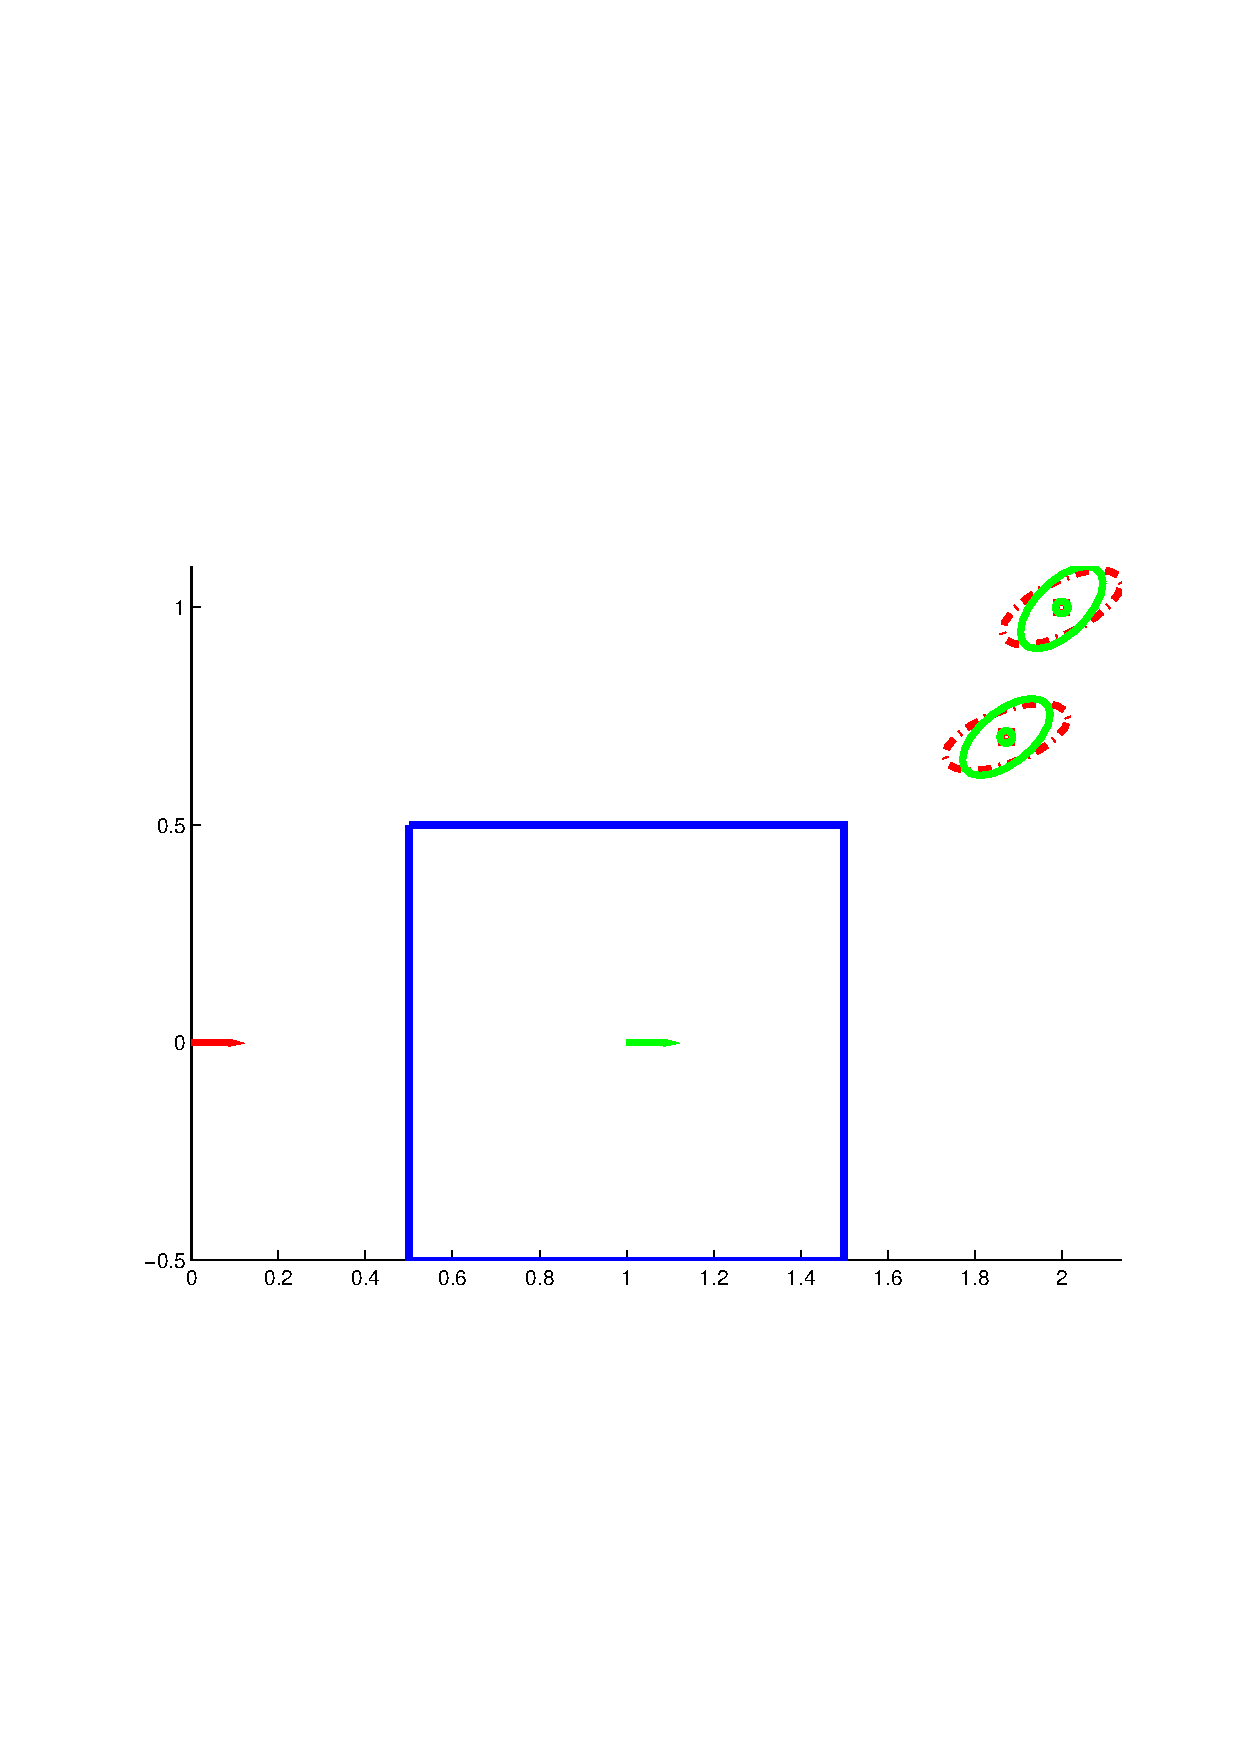
\includegraphics[width=6cm]{Pics/post_example}
\label{fig:post_example}
}
\subfigure[$p({\bf x} | {\bf u})$]{
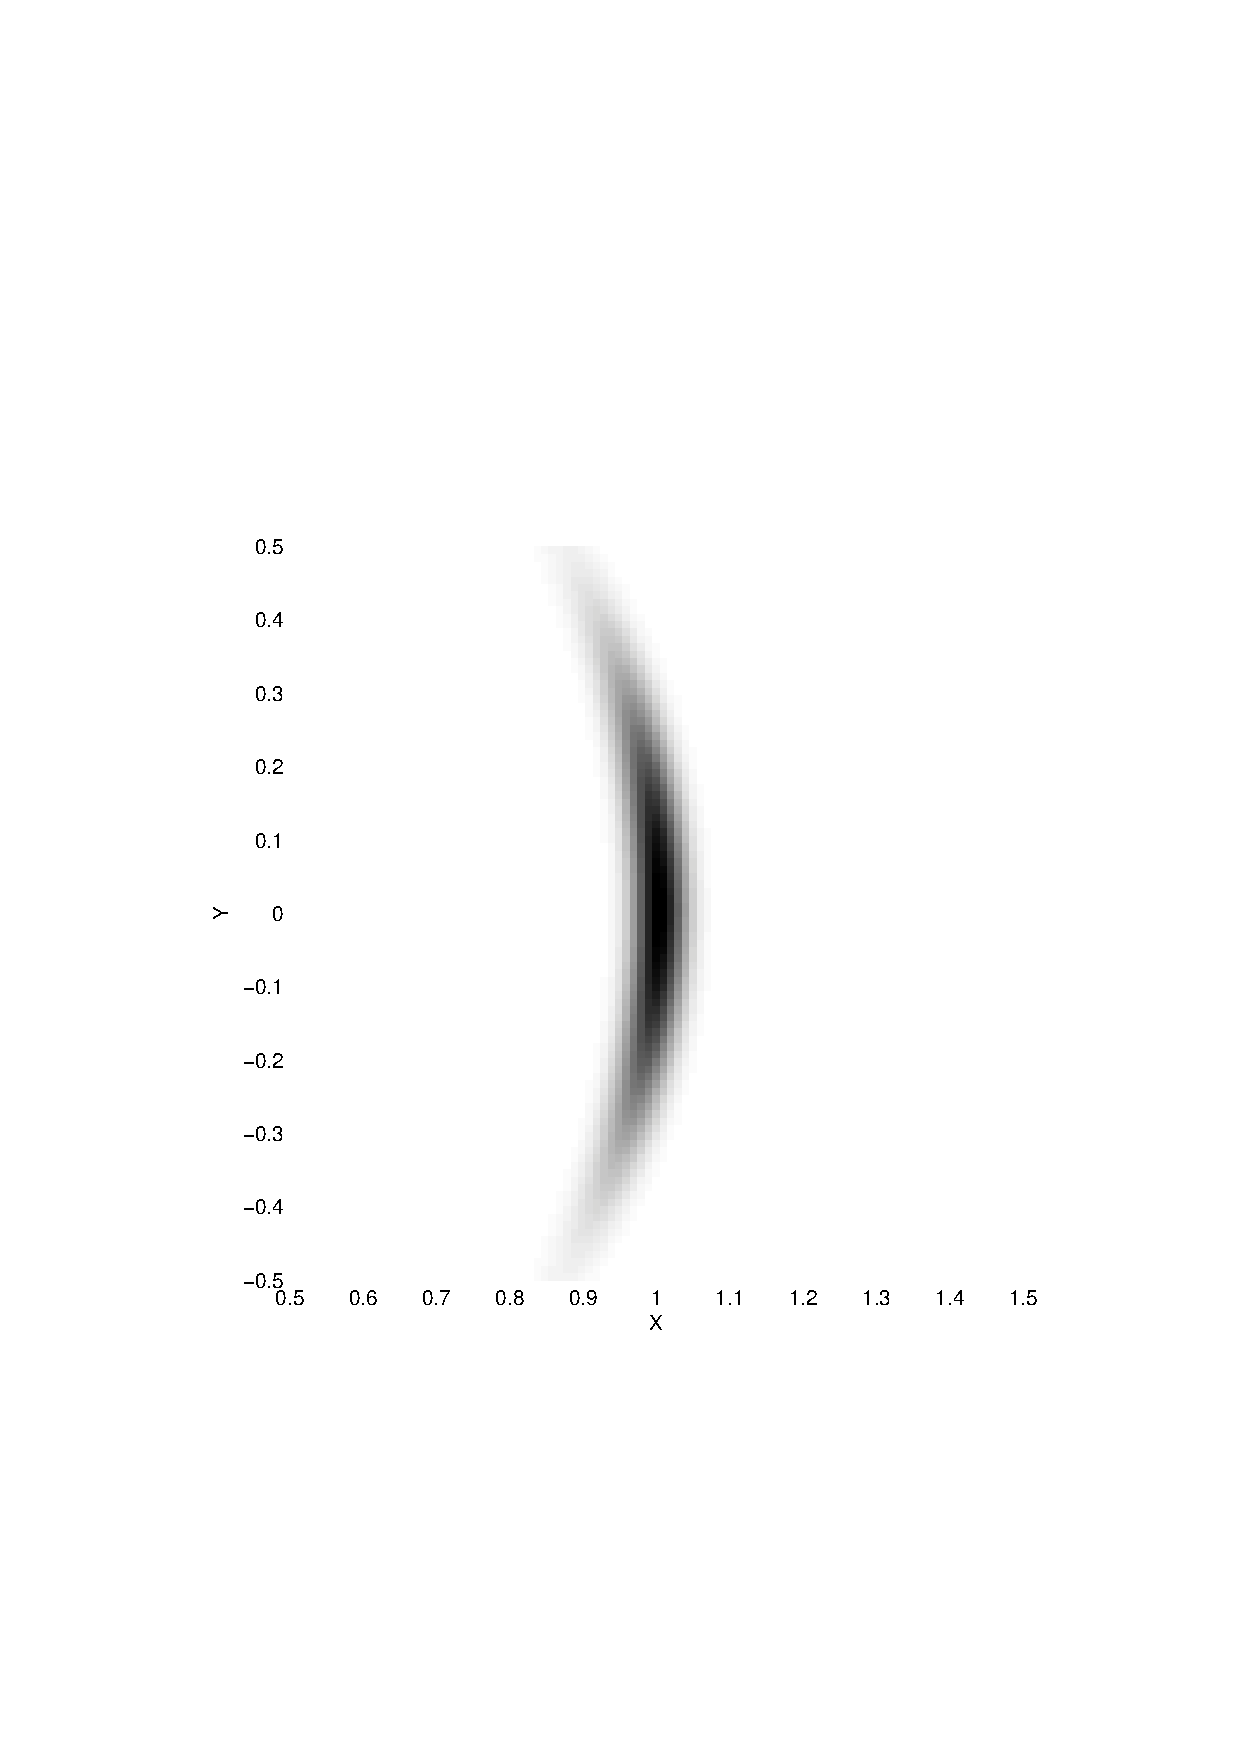
\includegraphics[width=6cm]{Pics/post_odo}
\label{fig:post_odo}
}\\
\subfigure[$p({\bf x} | {\bf z})$]{
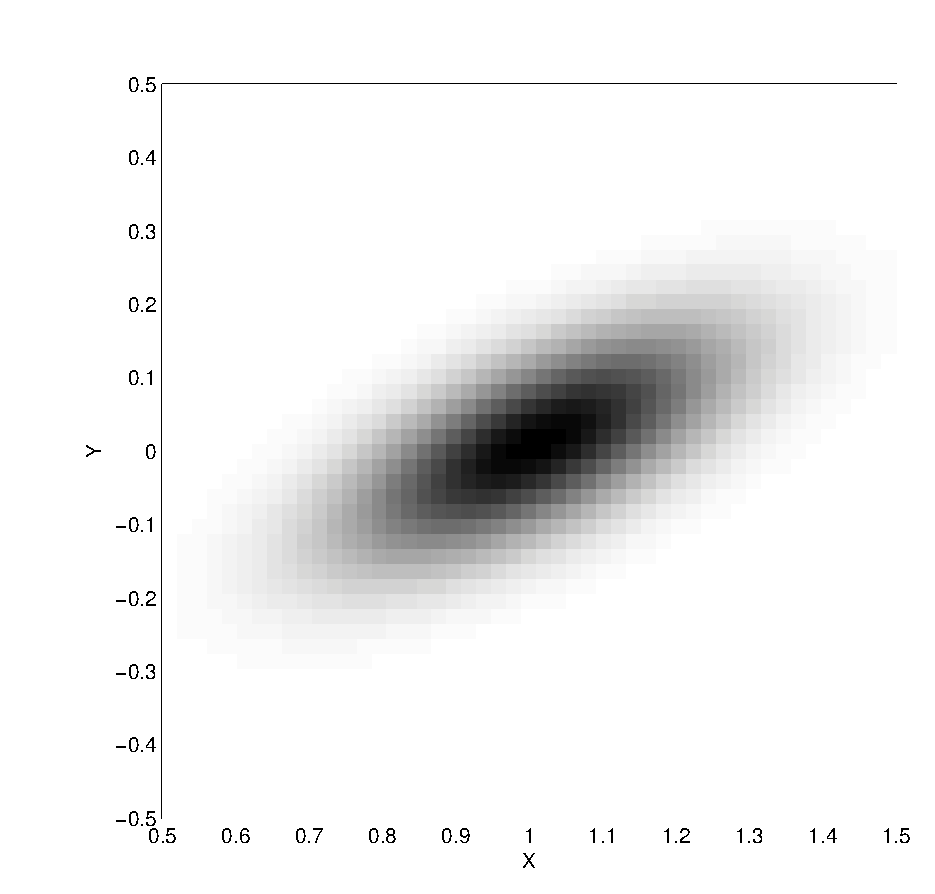
\includegraphics[width=6cm]{Pics/post_obs}
\label{fig:post_obs}
}\quad\space
\subfigure[$p({\bf x} | {\bf u},{\bf z})$]{
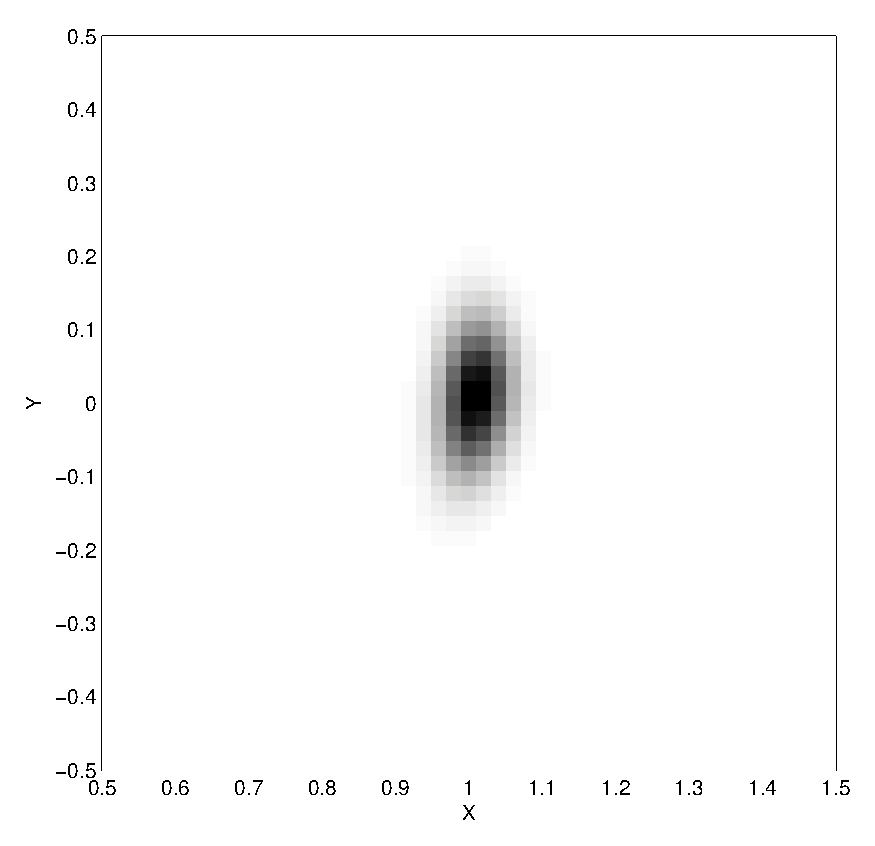
\includegraphics[width=6cm]{Pics/post_obsodo}
\label{fig:post_obsodo}
}
\end{center}
\caption{In \ref{fig:post_example} robot makes observation at point (0,0),
then moves 1 meter forward and makes another observation. The square
shows the region for which pose uncertainty was computed. The
resulting uncertainty just before second measurement is shown in
\ref{fig:post_odo}, the uncertainty due to the measurement is
\ref{fig:post_obs}, and the robot's uncertainty after incorporating
the measurement is \ref{fig:post_obsodo}.}
\label{fig:post_all}
\end{figure}

The main limitation of the EKF approach is the assumption that
uncertainty can be modelled as a Gaussian distribution. Many real life
systems are non-linear, as a result even purely Gaussian noise in
actuation or observation will result in a non-Gaussian posterior
distribution.  

\refFigure{fig:post_all} illustrates uncertainties involved in the 
robotic mapping system. The robot makes an observation at point (0,0),
then moves one meter forward and makes another observation at
approximately (1,0), see \refFigure{fig:post_example}. The environment
consists of just two landmarks at (2,0.5) and (2,1). We assume they
are distinct, so the robot knows the correspondences between the two
observations. The robot motion is a stochastic process, hence the
robot pose is not known exactly after the execution of the motion
command (in this case move forward 1 meter). The typical resulting
uncertainty for a robot with differential drive system is shown in
\refFigure{fig:post_odo}. As can be seen from the plot  this 
distribution is anything but Gaussian. The ``banana shape'' comes from
the fact that robot is uncertain about the direction of travel, as
well as the distance travelled. Even though the uncertainty about
the distance and direction is zero mean Gaussian, the effect this
uncertainty has on the pose of the robot is far from Gaussian.

\begin{figure}
\begin{center}
\subfigure[EKF ($1\sigma$)]{
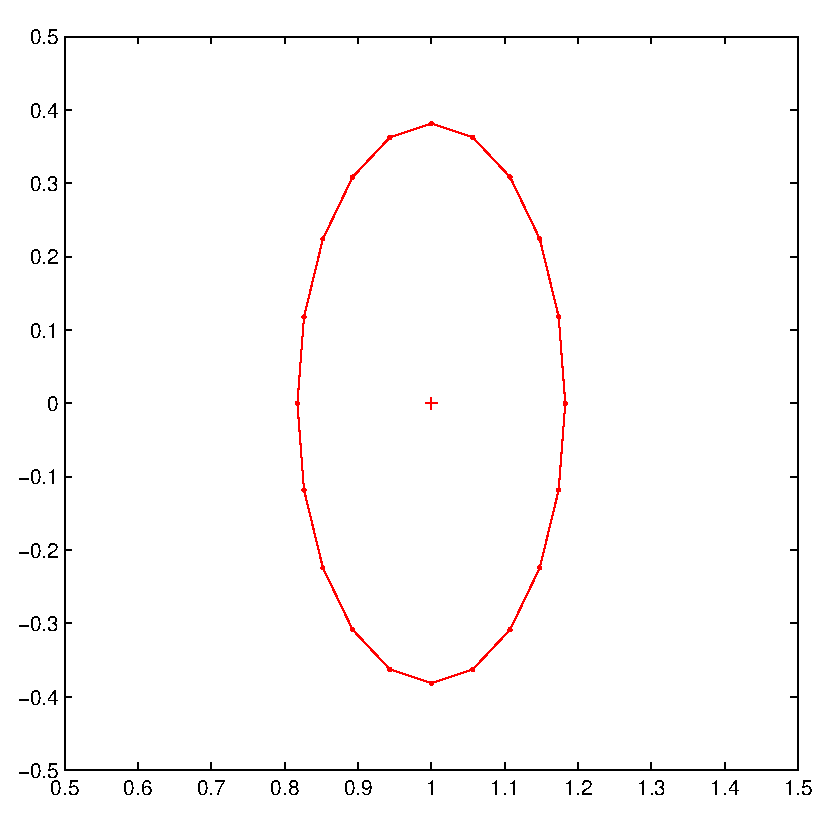
\includegraphics[width=6cm]{Pics/post_odo_ekf}
\label{fig:post_odo_ekf}
}\quad
\subfigure[Particle Filter]{
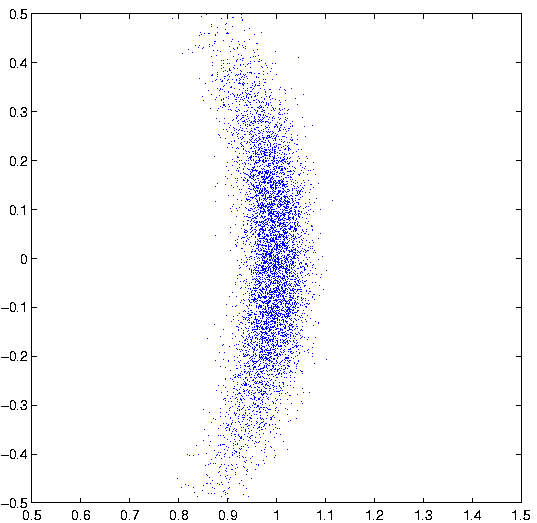
\includegraphics[width=6cm]{Pics/post_odo_pf}
\label{fig:post_odo_pf}
}
\end{center}

\caption{Modelling of the robot pose uncertainty,
 using EKF (a) and the particle filter (b).
}
\label{fig:post_ekf_vs_pf}
\end{figure}


After execution of the motion command the robot observes the landmarks
once more. Since the observations were not certain for both first and
second observation, the pose estimate that can be derived from the
measurements has a significant uncertainty. This is illustrated in
\refFigure{fig:post_obs}. The posterior distribution is non-Gaussian
in this case as well, although the difference is not as apparent as in
the motion example. The posterior distribution of the robot pose given
observations and control input is shown in
\refFigure{fig:post_obsodo}, and it is obviously non-Gaussian.
\refFigure{fig:post_ekf_vs_pf} illustrates the resulting uncertainty
computed by the EKF and particle filter algorithms after applying a
control input, as in example in \refFigure{fig:post_all}. One can see
that particle filtering captures the banana shape of the motion model
much better than the EKF.


\section{Localisation} 
\label{sec:Localisation}

%What is localisation
%Typically the robot
%uses a collection of sensors to collect observations of the 
%Why does the robot need to localise
%Topological vs Metric
%Subclasses of the localisation problem

Mobile robot localisation is the problem of estimating the pose of a
robot (location and orientation, in the case of a mobile robot moving
in a plane). Localisation is one of the fundamental problems in the
field of mobile robotics. It is considered one of the prerequisites
for providing autonomous capabilities for a mobile robot \cite{Cox91}.
The localisation algorithm can face three possible problems

\begin{itemize}
\item {\bf Position tracking}\\
      The robot's initial pose is known with relatively high
      certainty. The robot keeps track of its pose as it moves through a
      familiar environment.

\item {\bf Global Localisation}\\ 
      The initial pose of the robot is unknown, or is given by a
      probability distribution $p(\x{0}{}{})$ with high variance. As
      the robot moves through the environment and collects
      observations, it should be able to determine its pose.

\item {\bf Kidnapped robot}\\
      The robot is moving through the environment and is reasonably
      certain about its pose, suddenly it gets teleported to some
      other place within a known map, without being told. The robot
      should be able to detect that its estimate of the pose is no
      longer correct and re-localise.
\end{itemize}

Much research has previously concentrated on position tracking - in
fact many existing algorithms address only the first problem (see
review in \cite{Borenstein96}). Global localisation and the Kidnapped
robot problems have been addressed using multi-hypothesis Kalman
filters \cite{JensfeltKristensen01,Cox94}, Markov localisation
\cite{Fox99}, and Monte Carlo methods \cite{Thrun00j}.


\subsection{Problem Definition}

The problem of localisation can be thought of as a problem of
estimating the probability density distribution of robot pose
conditioned on the observation and control data.  This posterior is
typically called {\it Belief} and is denoted
\begin{equation}
  Bel(\x{k}{}{}) = p(\x{k}{}{} | \Uall{k-1}{}, \Zall{k}{}),
\label{eqn:localise_belief}
\end{equation}
where \Uall{k-1}{} is a set of all control inputs up to time $k-1$, and
\Zall{k}{} is a set of all observations up to time $k$. It is usually
desired to approximate the posterior recursively, otherwise one would
run into computation problems very quickly.  If we make a Markov
assumption that future data is independent of past data given the
robot pose is known, we have

\begin{eqnarray}
 p(\z{k} | \Zall{k-1}{}, \Uall{k-1}{})    &=& p(\z{k} | \x{k}{}{}) \\
 p(\x{k}{}{} | \Zall{k-1}{}, \Uall{k-1}{})&=& p(\x{k}{}{} | \x{k-1}{}{}, \U{k-1}{}).
\end{eqnarray}

We can transform \refEquation{eqn:localise_belief} into a recursive
formula, by applying Bayes' rule (see \cite{Thrun00j} for a derivation)

\begin{equation}
Bel(\x{k}{}{}) = \eta p(\z{k} | \x{k}{}{}) \int 
                     p(\x{k}{}{} | \x{k-1}{}{}, \U{k-1}{}) 
                     Bel(\x{k-1}{}{}) d \x{k-1}{}{},
\label{eqn:localise_recursion}
\end{equation}

where $\eta$ is a normalisation constant. To implement the recursive
rule in \refEquation{eqn:localise_recursion} one needs to know the
distributions $p(\z{k} | \x{k}{}{})$ and $p(\x{k}{}{} | \x{k-1}{}{},
\U{k-1}{})$. These distributions are generally referred to as {\it
observation} (or sometimes {\it perception}) and {\it motion} models,
respectively. 

The motion model reflects the uncertainty in robot dynamics, so it is
generally independent of time $k$. The observation model is a function
of robot sensors and of the environment. If sensor characteristics do
not change with time and if features in the map are static (a common
assumption), the same observation model can be used for every time
step.

\subsection{Common Approaches to Metric Localisation}

%EKF
Several approaches to localisation have been proposed. One family of
algorithms use the Extended Kalman Filter\cite{Jensfelt99}. Approaches
based on the EKF linearise motion and observation models and
approximate the posterior distribution with a Gaussian. While being
computationally efficient, EKF based approaches have plenty of
drawbacks. First they are not capable of global localisation, hence
the initial pose of the robot should be known in advance with
relatively high confidence. An EKF is only capable of representing a
unimodal posterior distribution, meaning that in an ambiguous
situation only one of the position hypotheses can be considered. This
can lead to localisation failure if the wrong choice is made.

A mixture of Gaussians model can be used to allow for multiple
hypotheses \cite{JensfeltKristensen01,Cox94}. But the problems arising
from linearisation are still present in these approaches.

%Markov
Markov localisation uses a grid to model the posterior distribution
\cite{Fox99}. This approach is capable of global localisation, and can
deal with the kidnapped robot problem as well. Fox \etal\ \cite{fb99}
have shown that Markov localisation works well, even in highly crowded
environments. The main advantage of this approach is the ability to
model any complex distribution. This makes the algorithm more robust
and allows for global localisation. Drawback include finite grid size,
computational demand and sophisticated implementation to optimise the
observation update and increase resolution ``on the fly''.

%MCL
Monte Carlo Localisation (MCL), also known as particle filtering,
algorithms model the posterior distributions as a set of particles
\cite{Thrun00j, JensfeltAustinWijk00b}. MCL is capable of
approximating any probability distribution, including multi-modal
distributions. It can perform global localisation and can solve the
kidnapped robot problem. Unlike grid-based algorithms, MCL has a
floating point resolution for robot pose, and so can give more
accurate pose estimate. Although it is computationally more demanding
than EKF approaches, it is my belief that the increased robustness of
this algorithm makes it worth the additional computational resources
required. The computational complexity of the MCL algorithm is $O(N)$
in the number of particles used to represent the robot
pose. Increasing the number of particles will result in greater
accuracy and robustness. It is therefore easy to trade off the
computational resources against performance.

\section{Simultaneous Localisation and Mapping}
\label{sec:SLAM}

\subsection{SLAM Problem}

This section introduces the problem of Simultaneous Localisation and
Mapping.

A robot starts at time 0 at location \x{0}{}{}, executes a series of
motion commands $\Uall{k}{} = [\U{0},\U{1}...\U{k}]$ and collects a
set of observations at every step
$\Zall{k}{}=[\z{0},\z{1}...\z{k}]$. In practice observation and motion
commands are not synchronised, however this can be easily accommodated
for in the implementation. It is therefor commonly assumed that
observation and motion happen at the same discrete time interval.
Control and perception of the robot are subject to noise.

\SILENT{$[\mape{}{}{1},\mape{}{}{2}...\mape{}{}{n}]$}

SLAM seeks to find the true path of the robot up to time $k$,
$\Xall{k}{}{} = [\x{0}{}{}, \x{1}{}{}, ... \x{k}{}{}]$, and the true
model of the environment, $\map{k}{}{}$. Since there is an inherent
uncertainty in the robot's observation and motion, one generally
cannot give an exact description of the robot's path, and a map of the
environment. However, it is possible to construct a probabilistic
model that would assign a likelihood to every path-map combination,
given all of the available observations, control inputs and the
initial pose of the robot:

\begin{equation}
 p(\Xall{k}{}{}, \map{k}{}{} | \Zall{k}{}, \Uall{k}{}, \x{0}{}{})
\label{eqn:map}
\end{equation}

If one makes an assumption that odometry errors are independent of the
observation errors and of the environment model, one can separate the
model into an observation and motion parts, so we define:

\begin{enumerate}

\item The model of the robot's motion $P(\x{k}{}{} | \Uall{k}{})$. \\
If one makes a further assumption that past odometry errors have no
effect on future errors, one can represent robot motion as a Markov
process, with probability distribution 
\begin{equation}
 P(\x{k}{}{} | \Uall{k}{}) \equiv p(\x{k}{}{}| \x{k-1}{}{}, \U{k})
\end{equation}


\item The model of the robot's perception
$p(\z{k}| \x{k}{}{},\map{k}{}{}, \Zall{k}{})$.\\
Here again an assumption is made that errors in the measurements are
independent from past errors.

\SILENT{
, and also that only one landmark has
effect on the measurement, presence or lack of other map elements does
not affect our observation of the landmark.}

\begin{equation}
p(\z{k}| \x{k}{}{},\map{k}{}{}, \Zall{k}{}) \equiv 
  p(\z{k}| \x{k}{}{},\map{k}{}{})
\end{equation}

\SILENT{
\item The data association model (depends on the environment and the sensor)
\begin{eqnarray}
 p(\z{k} \equiv noise), \\
 p(\z{k} \equiv new | \x{k}{}{}, \map{k}{}{}),\\
 p(\z{k} \equiv \mape{}{}{\asc{k}} | \x{k}{}{}, \map{k}{}{}).
\end{eqnarray}
}

\end{enumerate}

Equipped with the knowledge of these distributions one can in
principle compute the exact posterior, by considering every possible
path, map and data association decision combination. In practice,
however, computing such a distribution exactly is not possible due to
high dimensionality and non-linearity of the system. Reasonably good
approximations can, however be obtained, and better yet they can be
computed incrementally in real-time.

The two most common approaches to solving the SLAM problem are the EKF
based algorithm and a particle filter algorithm called ``FastSLAM''.

\subsection{Kalman Filter Approach}
The Extended Kalman Filter approach treats the SLAM problem as a state
estimation problem, where the state consists of the robot pose and
locations of all landmarks. Usually the number of features is not
known in advance, so most implementations have some provision for
adding new elements to the map as new observations arrive. EKF SLAM
requires linearisation of the robot's motion and perception models, so
that the estimation error can be modelled by a Gaussian distribution.
The computation complexity of the algorithm is $O(K^2)$, where $K$ is
the number of features in the map \cite{ekf_slam}.

Sub-optimal implementations reduce this complexity significantly by
restricting the update of the covariance matrix to a local map
(Compressed Filter) \cite{williams:acra2001}. The most important
limitation of the EKF approach is its inability to model multiple data
association decisions. Every observation has to be classified as
either noise, a new feature or an observation of an existing feature.
It is possible to postpone the final decision by running multiple
Kalman filters in parallel. Alternatively one can try to improve data
association, for example using the Joint Compatibility test
\cite{neira01:_data_assoc_stoch_mappin_using}.  Both approaches reduce
the probability of an incorrect data association decision, but
ultimately produce a unimodal distribution.

\subsection{Particle Filter Approach}
FastSLAM uses particles to approximate the posterior distribution
\cite{fastslam}. Every particle maintains it's own path,
data association decisions and the resulting map. The map is a
collection of independent landmarks. Their locations are estimated
using Kalman filters, one for every landmark. FastSLAM requires
linearisation of the perception model, but it samples directly from
the motion model. As a result, no change to the motion model is
required. FastSLAM can be implemented in $O(M\log K)$, where $M$ is
the number of particles, and $K$ is the number of landmarks. FastSLAM
produces a better estimate of the posterior distribution, given enough
particles. The main advantage of FastSLAM is its ability to handle
multiple data association decisions \cite{Montemerlo02d}, which we
believe makes it a more robust algorithm. It is also a conceptually
straightforward approach.

%We therefore chose to use FastSLAM to perform local mapping tasks.


\section{Loop Closing}
\label{sec:back_loop}
%Problem definition
  % Detect
  % Correct

The problem of loop closing, or revisiting, arises when mapping a
large cyclic environment. As the robot moves through an unexplored
environment while building the map, it becomes more and more uncertain
about its pose relative to the regions it mapped in the past. The
increase in the uncertainty makes it hard for the robot to detect when
it comes back to the region it has mapped already. Failure to detect
revisiting results in an inconsistent map.

In order to build a consistent map, the robot needs to be able to
detect the places it has been to before and correct its estimate of
the path along the loop. The problem of mapping large cyclic
environments has been addressed by several researchers.


%what is there now
  %Lu Milios (scan matching + optimisation)
  %Gutman   (scan matching + confirm + handles high uncertainty)
  %Thrun's  (EM)
  %Fergusson (EKF mines)
  %Atlas


Lu and Milios \cite{lu97:_global} propose an algorithm they call
``consistent pose estimation''. The algorithm uses laser scan matching
and linearised global optimisation over scan poses to build a scan map
of the environment in a single global frame. The approach builds a
network of robot poses at which a laser scan has been taken. The poses
are connected by ``weak'' and ``strong'' links. The links represent
the spatial relations between poses. Weak links are derived from
odometry, and strong links are derived from the scan matches. The
algorithm then finds a global configuration of the poses of the places
by minimising a cost function. If one thinks of links as springs, the
algorithm finds the configuration that reduces the sum of forces
exerted by the springs. Spatial relations are modelled by Gaussians,
and the cost function is the sum of the Mahalanobis distances.

The method by Lu and Milios is very sensitive to the initial estimate
of the robot pose just before loop closing. Since the pose estimate is
derived from the local scan matching and odometry, it can, in
principle, have unbounded error. If the initial estimate is too far
from the real robot pose, the algorithm often converges to local
minima that are not correct. Another problem with this method is the
computational complexity, which is $O(N^3)$ in the number of poses.

Konolige and Gutman
\cite{konolige99:_increm_mappin_large_cyclic_envir} provide a method
based on the ideas of Lu and Milios, but try to address these
problems. Instead of using single laser scan to find relations between
places they use a map correlation technique \cite{konolige99}. This
makes the system more robust to false correspondences. After detecting
loop closing, the algorithm runs consistent pose estimation. 

Another interesting scan matching based mapping technique is
\cite{fergusson2003} by Ferguson \etal. In this approach loop closing
can be undone if the observations further down the track do not
support it.

Thrun \etal \cite{slam_thrun98b,Thrun98a,thrun98:_probab} suggest an
approach that uses an Expectation Maximisation (EM) algorithm for
constructing maps of cyclic environments. The algorithm is given a
relatively small set of observations of sparsely positioned non-unique
landmarks and a set of all control inputs. In the expectation step the
algorithm computes the most likely robot path given the map and the
data. In the maximisation step the most likely map is computed, given
the robots path from the E-step. The Expectation and Maximisation
steps are repeated until the map converges to the maximum likelihood
solution. This algorithm cannot be implemented in real-time, because
it needs to have access to all of the future and past data to
determine the robot pose at any given time.

All of the methods presented so far build a map of the whole
environment in a single global reference frame. Recently, Bosse \etal\
\cite{bosse02atlas} suggest a mapping approach, \Atlas, that does not
require a global reference frame. The map structure used in this
approach is a hybrid topological/metric map.  Each node is a local map
and every link in the topological map represents a spatial
relationship between the two places it connects.  Spatial
relationships are derived from the residual robot pose uncertainty of
the mapping process used to build the local maps. The underlying
mapping module is EKF SLAM with line and point features extracted from
either laser or sonar range data. The uncertainty in spatial
relationships are modelled as Gaussians.

\Atlas\ uses a combination of map matching and uncertainty projection
to detect when the robot re-enters a previously explored
area. Uncertainty projection computes the relative poses between the
two non-adjacent local maps. If according to this estimate, the two
maps might be overlapping, \Atlas\ tries to find the landmark
correspondences between the two maps. If the two maps match, the new
link is added to the topological map. The pose relation for this link
is computed from the landmark correspondences. \Atlas\ does not
attempt to correct spatial relations between the map frames along the
closed loop. In order to decrease the probability of incorrect data
association, \Atlas\ runs several hypotheses at any given time. If,
after closing the loop, the observations do not match the map well
enough, the loop closing hypothesis will be discarded in favour of the
new map hypothesis.

The main advantage of \Atlas\ is the map structure it uses. Moving
away from the single reference frame allows the mapping of large
environments with huge cycles in real time. There are some
deficiencies in their approach though. For instance, when the robot
returns to the previously mapped region it gains new knowledge about
relative positions of the local maps. The robot can use this knowledge
to update the links in the map. \Atlas\ does not perform this update
because of the computational requirements involved, although the
authors mention that such update can be performed after the mapping is
complete. \Atlas\ uses metrics to test loop closing hypotheses. These
metrics do not necessarily correspond to the true likelihood, making
it difficult to predict the behaviour of the algorithm in a new
environment. 

\SILENT{how do you tune these metrics if you have a different sensor,
  than what they used?}

\section{Summary}

The past few decades of mobile robotics research provide us with
the tools for mapping and localisation. Unfortunately, existing
algorithms work only in relatively small environments. The main
limiting factors are:

\begin{itemize}
\item The computational burden: as size of the environment grows, so do
  the computational requirements of existing algorithms.

\item The data association problem in the face of uncertainty: 
   in large environments the uncertainty of the landmarks far away
  from the origin is high. That makes it difficult to perform correct
  data association.

\end{itemize}

Various optimisation techniques and faster hardware can expand the
capabilities of existing algorithms, but to really overcome these
limitations new map representations are required. In particular new
ways to model uncertainty should be explored. Some recent research in
this area include \cite{bosse02atlas,fergusson2003}.

% LocalWords:  Kalman odometry EKF FastSLAM Bayes MCL Lu Milios Konolige Gutman
% LocalWords:  Thrun Bosse Ferguson resampling Gaussians linearisation



\chapter{HTSLAM Map Structure}
\label{chpt:MapStructure}
HTSLAM models the map as a hybrid topological-metric structure: the
environment is divided into a number of regions, and a local metric
map is built for each region. The relative poses of the regions are
stored in a topological structure. There is no global reference
frame. Only relative poses of the nearby regions are stored.

The motivation for the structure comes from a few sources. First,
dividing the world into a set of local maps appears to approximate the
way that humans reason \cite{psycho_kuipers82}. Second, is to ensure
that the mapping scheme scales to large environments.  The scalability
limitations of a single map SLAM methods are well known
\cite{guivant03,guivant01,guivant02} and prohibit real-time SLAM for
maps of practical size.  The third and final motivation is that a
robot does not require a single, global, metric description of the
world.  For example, in the ``fetch me a beer from the refrigerator''
task, there is no need for the robot to know the position of the
fridge while it is in the living room.  The robot only needs to know
the position of the fridge when it is near to the fridge.

This chapter describes the HTSLAM approach to map modelling.  Some
aspects of the map design are motivated by the mapping procedures
developed in chapter~\ref{chpt:Mapping} and so may only become fully
clear after reading chapter~\ref{chpt:Mapping}. The following section
describes the overall map structure.  Section~\ref{sec:local_map}
presents the methods used for modelling uncertainty within each local
map and section~\ref{sec:link} describes the methods used to model the
uncertainties of the topological links between maps.  Finally,
section~\ref{sec:region} discusses methods for defining the shape and
extent of each local region.

\section{Hybrid Map structure}
\label{sec:HM_structure}

\begin{figure}
\begin{center}
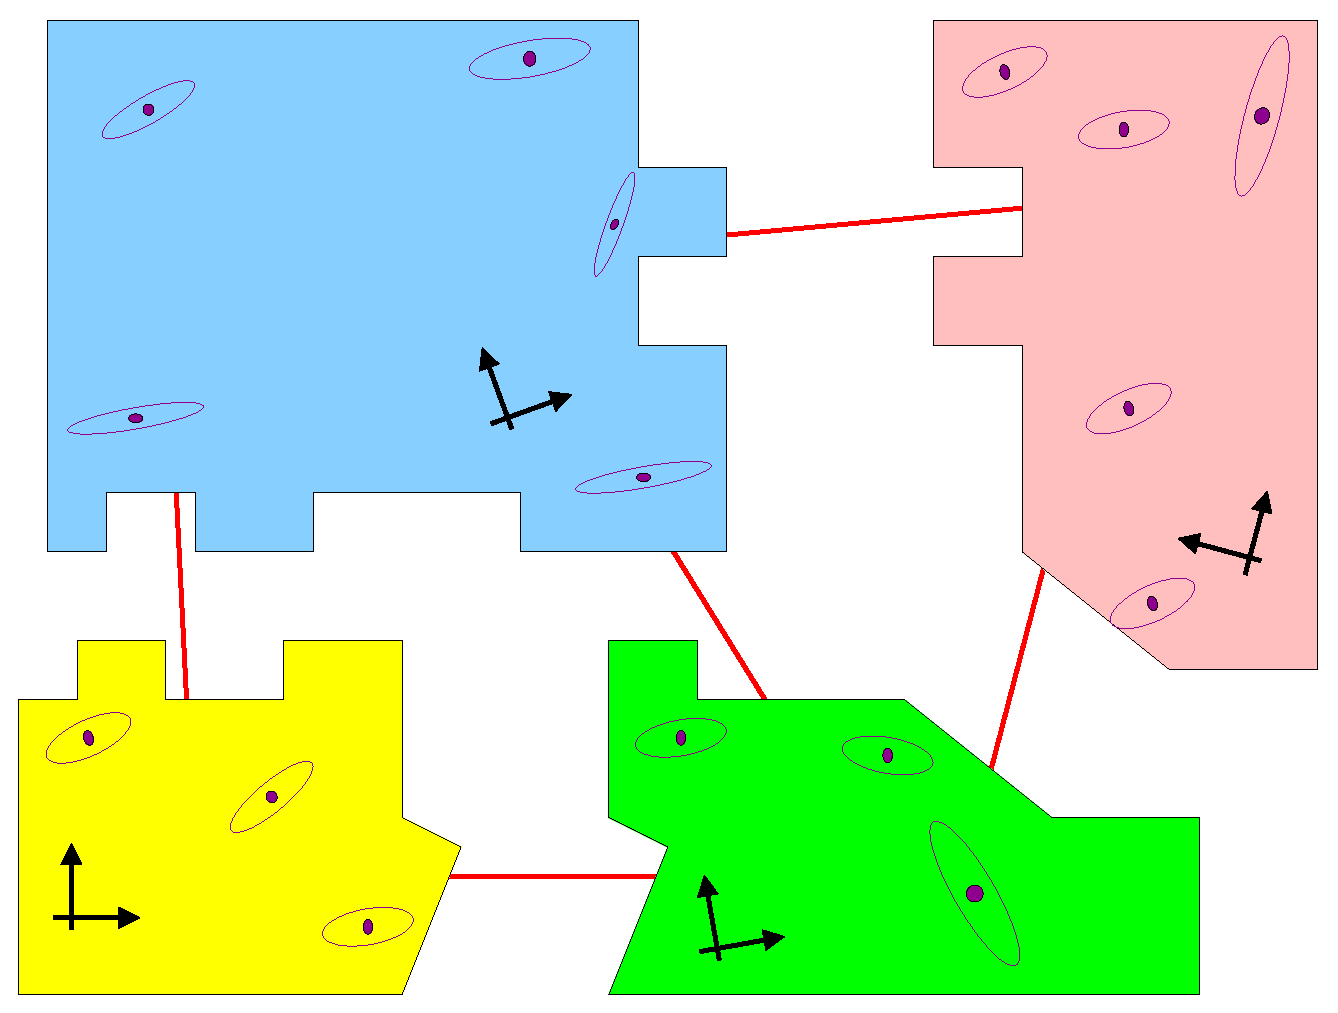
\includegraphics[width=10cm]{Pics/fig_map_structure}
\end{center}
\caption[Overview of HTSLAM map structure.]
{Overview of HTSLAM map structure. Each region has it's own
coordinate frame. The local map is built for every region (ellipses
erepresent landmarks). }
\label{fig:htslam_structure}
\end{figure}

\begin{figure}
\begin{center}
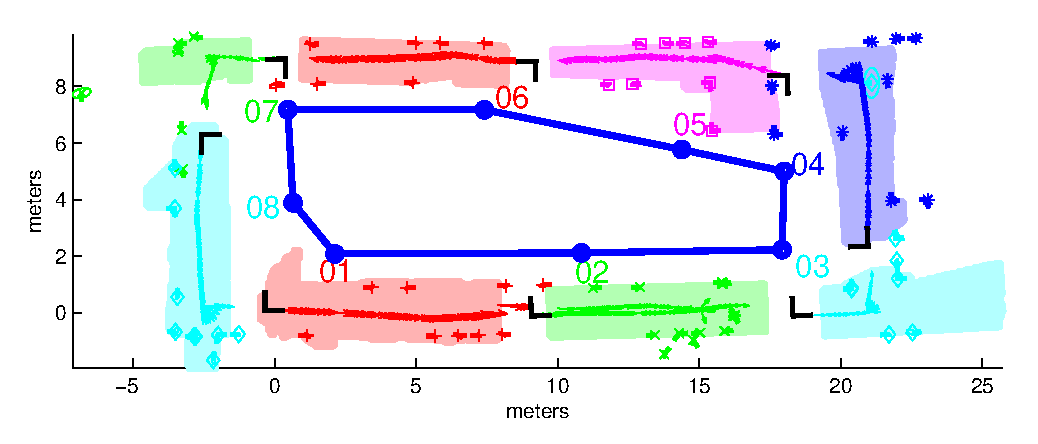
\includegraphics[width=14cm]{Pics/map_example_indoor}
\end{center}
\caption{Example of HTSLAM map for indoor environment}
\label{fig:htslam_structure_indoor}
\end{figure}


\begin{figure}
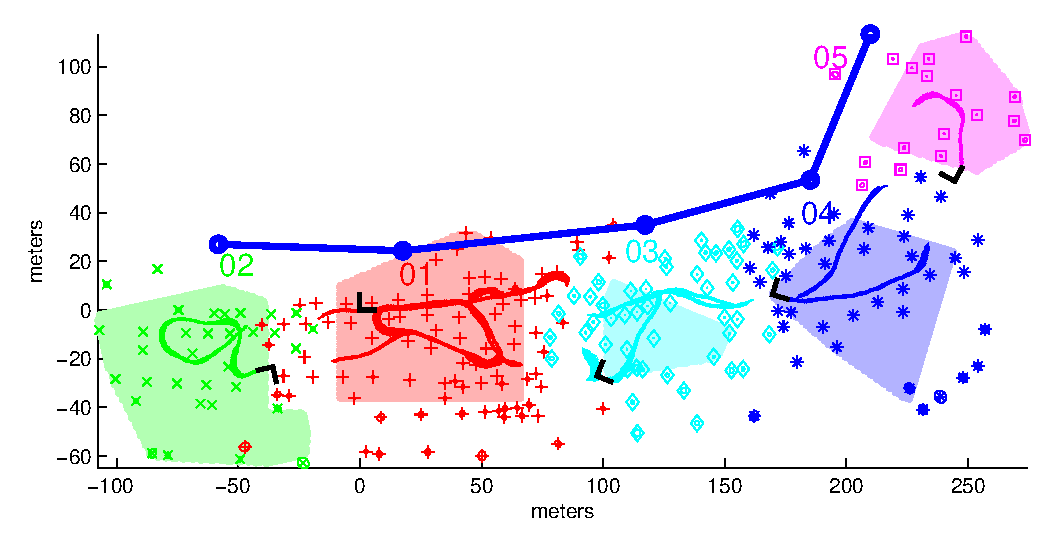
\includegraphics[width=14cm]{Pics/map_example_outdoor}
\caption{Example of HTSLAM map for outdoor environment}
\label{fig:htslam_structure_outdoor}
\end{figure}

In HTSLAM, a map is a connected graph. Every node of the graph
corresponds to a region within the environment. Each node has its own
reference frame and stores a local, metric map of the region and some
representation of the extent of the region in the local coordinate
frame. An example of HTSLAM map is given in the
\refFigure{fig:htslam_structure}. Note that there is no global reference
frame. The edges of the graph represent the stochastic coordinate
transformation between adjacent local maps
only. \refFigure{fig:htslam_structure_indoor} shows an example of an
HTSLAM map for indoor environment, and
\refFigure{fig:htslam_structure_outdoor} for an outdoor environment.

The structure used in HTSLAM is similar to that of \Atlas\
\cite{bosse02atlas}, however HTSLAM uses different uncertainty
representations, both for the coordinate transformations between
adjacent map frames and for the local maps.  \Atlas as a framework
allows to use arbitrary mapping model, however the two implementations
that have been published include EKF SLAM and scan matching.  \Atlas\
models the links or transitions between maps as Gaussian, and
therefore requires that the spatial uncertainty of the mapping module
is represented as a Gaussian.  On the other hand, HTSLAM uses
Rao-Blackwellised particle filter for the local maps (like FastSLAM),
permitting multi-modal modelling of the local map. HTSLAM also models
the transitions between maps using sets of particles.

A further difference between \Atlas\ and HTSLAM is that HTSLAM
maintains map extent information for every local map. This extra data
allows HTSLAM to perform map transitions and loop closing in a more
elegant way (as will be discussed later in
Chapter~\ref{chpt:LoopClosing}). In addition, HTSLAM explicitly
models the multiple hypotheses that arise during mapping, including
during loop closing, giving a more intuitively appealing and robust
approach.

The details of the uncertainty representation, both for each local map
and for the transitions between maps are discussed in the next two
sections.  Section~\ref{sec:region} discusses methods for
determining the extents of each local map.

\section{Modelling Uncertainty within a Local Map}
\label{sec:local_map}

To understand how uncertainty is represented within the local map, one
needs to be familiar with FastSLAM \cite{Montemerlo02d}, the mapping
scheme we use. An overview of FastSLAM was presented in
chapter~\ref{chpt:Overview}. In short, FastSLAM uses particles to
sample the possible paths of the robot. A map is built for each
path. Particles are evaluated based on how well the measurements match
the map.  Regular resampling is used to prune out unlikely paths.

The state $\s{k}{a}{m}$ of the $m$-th particle in the local map $a$
at time $k$ consists of the path of the particle within this local
frame, denoted \Xall{k}{a}{m}, and the map of the local environment
conditioned on the path, denoted \map{k}{a}{m}, i.e.
\begin{eqnarray}
 \s{k}{a}{m}    &=& [\Xall{k}{a}{m}, \map{k}{a}{m} ]\\
 \Xall{k}{a}{m} &=& [\x{0}{a}{m}, \x{1}{a}{m}, ... \x{k}{a}{m}]\\
 \map{k}{a}{m}  &=& [\mape{a}{m}{1}, \mape{a}{m}{2}, ..., \mape{a}{m}{n}],
\end{eqnarray}
where $\x{k}{a}{m}$ is the pose of a robot for the $m$-th particle at
time step $k$ in local map $a$ and $\mape{a}{m}{n}$ is the position of
an $n$-th landmark in local map $a$. The landmark position is a
stochastic variable, described by a Gaussian distribution. Note that
one does not have to store the whole path of a particle, since only
the most current pose of the particle is used in the mapping process.

A map is a probability distribution
$p(\map{k}{a}{m}|\Xall{k}{a}{m},\Zall{k}{a})$. If one makes an
assumptions that the map consists of landmarks, and that observations
are independent, then one can represent a map as a set of independent
landmarks, each conditioned on the path of a particle
$p(\mape{a}{m}{}|\Xall{k}{a}{m},\Zall{k}{a})$ (note that there is a
different map for each particle). FastSLAM approximates
$p(\mape{a}{m}{}|\Xall{k}{a}{m},\Zall{k}{a})$ with a Gaussian.  For
point landmarks, the distribution is a two-dimensional Gaussian
(location of the landmark on the plane). However, other landmark
characteristics can also be incorporated into the stochastic
variable. For example, if one builds a map of trees, the landmark
might have one extra parameter for the diameter of the tree trunk.
Note that since there are multiple particles, the actual posterior
distribution of the landmark is more complex than just a Gaussian. In
this thesis we will confine ourselves to planar motion. The results
however can be readily extended to full three-dimensional motion. Note
that, since the landmarks are estimated independently (in FastSLAM),
there is no need to maintain the global covariance matrix for the
whole map.

Each particle makes its own data association decisions. As a result,
the FastSLAM captures not only the uncertainty arising from the
continuous variables like robots' pose and the sensor measurements,
but also uncertainty due to discrete data association decisions.  This
uncertainty is not represented in the EKF approaches \cite{ekf_slam}.
The ability to capture this uncertainty is a big advantage, since in
most real-life situations the data association is ambiguous.

When mapping of a given local map is complete, the maps of all
particles alive at the time are stored within the local map. This set
of maps is effectively a sample from all the possible maps, given the
observations and odometry during the time robot was in the region.
Due to use of importance sampling, the sample from the maps is
expected to contain the most probable paths and their associated maps
(which are expected to be the better maps).

\section{Modelling Link Uncertainty}
\label{sec:link}
%Uncertainty of transformations

\begin{figure}
\begin{center}
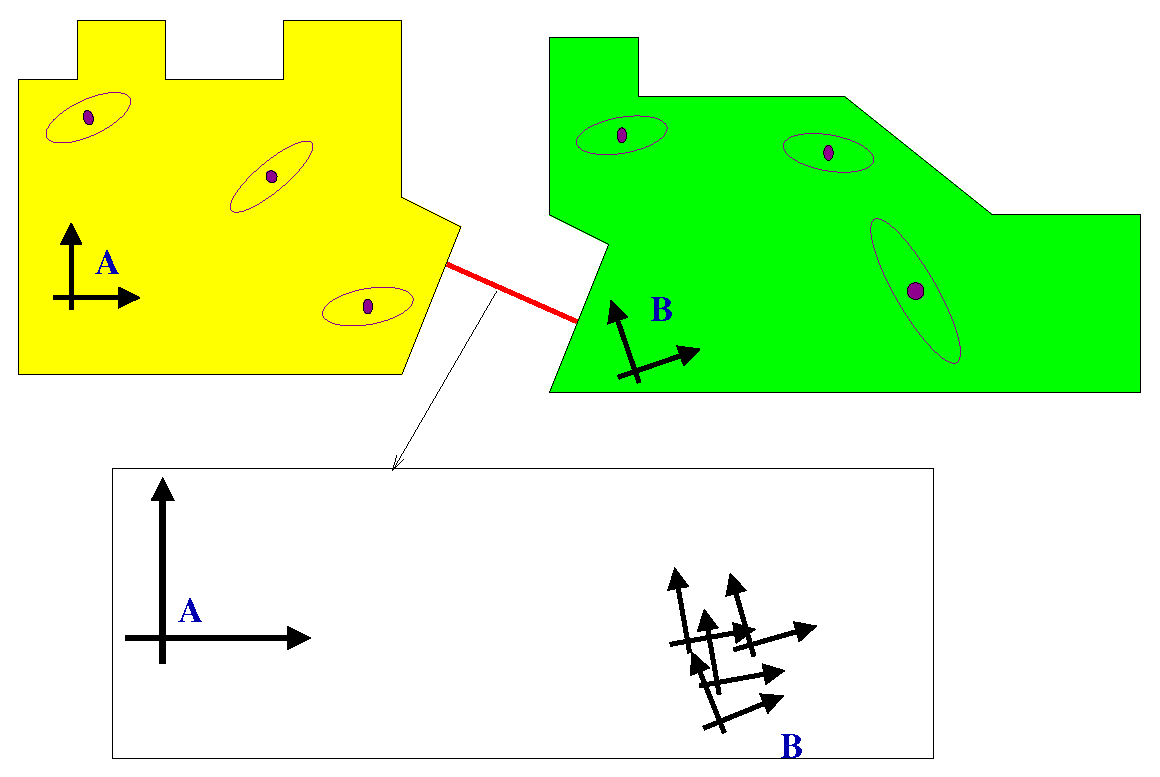
\includegraphics[width=10cm]{Pics/fig_transition_model}
\end{center}
\caption[Modeling transition distribution]
{Relative locations of the adjacent maps are represented by a
  set of particles.}
\end{figure}

The spatial relationships between adjacent local maps are each
represented by a set of particles.  As is common in SLAM
implementations, whenever a new map is started, the assumption is made
that the current location of the robot is precisely known in the new
map's coordinate frame.\footnote{Often it is assumed that the robot is
at the origin.  Here the position of the robot is chosen to place the
origin of the coordinate frame suitably for describing the local map
extents.} Thus, the transition between the old and the new map can be
most directly computed from the estimate of the robot pose in the old
map (a set of FastSLAM path particles) and the pose in the new map
(known by assumption). The transition is then a stochastic variable
which is most easily represented using particles. This is the chief
motivation for using a particle representation for the
transitions: the choice of representation makes the process of adding
new maps straightforward.

Note that when closing loops or, more generally, re-visiting maps,
there is no such easy method for transition determination and samples
must be taken from other distributions. For example, when closing
loops in HTSLAM, transition samples are taken from the results of map
matching (landmark matches are used to provide an estimate of
the transition function).

In general transitions and maps are not independent,
hence a joint probability needs to be stored. For adjacent maps $a$
and $b$ a joint probability distribution
$\prob{\map{}{}{a},\tr{}{a}{b}, \map{}{}{b}}$ is stored. Effectively,
the transition between the two adjacent maps captures a three-way
relationship between the two maps and the relative pose of the
reference frames of the two maps in a probabilistic manner. The exact
mechanism used to store the probability densities is described in more
detail in chapter~\ref{chpt:Mapping}.

It is worth noting that it is possible to derive the joint
probability $\prob{\map{}{}{a},\tr{}{a}{b},\map{}{}{b}}$ even for
non-adjacent maps $a$ and $b$ by merging probability densities along
the topological path joining the two maps.  The presence of loops in
the topological structure implies multiple paths between some of the
local maps. Therefore $\prob{\map{}{}{a},\tr{}{a}{b},\map{}{}{b}}$ can
be derived in several possible ways from the HTSLAM structure. This
adds a constraint to the HTSLAM structure, which will be discussed in
more detail in the chapter on loop closing(Chapter~\ref{chpt:LoopClosing}).

Let us define the coordinate transform using the \transit\ operator
\begin{equation}
\x{k}{}{b} = \x{k}{}{a} \transit \tr{}{a}{b}.
\end{equation}
This operator projects the pose of robot from one coordinate frame to
another.


\section{Defining Region Boundaries}
\label{sec:region}

Each region has its own ``area of influence''. This area is defined by
a grid map in the local reference frame. The size of the grid cells is
in the order of the robot's footprint, there is no need to have a
higher resolution. Regions who are neighbours in the topological
sense, have their region boundaries cropped in such a way as to
minimise the overlap. Since the grid maps are defined in local
coordinates, one needs to transform grids from one reference frame to
another. Since relative poses of the neighbouring maps are known with high 
certainty, the transformation is performed using the mean of the relative 
poses of the two regions.

By limiting the area of the local map, the HTSLAM algorithm achieves
two major goals: firstly the computation requirements per local map
are bounded, since there is a finite number of landmarks in a finite
area, secondly the residual uncertainty of the robot pose within the
local region is bounded.

TODO: accentuate the difference in approach from Atlas, that
constantly monitors the pose uncertainty/performance of the
mapper/size of the map.


DELETE BELOW THE LINE\\
===============================

One of the important problems for HTSLAM is dividing the environment
into local maps. Ideally each local map should correspond to a unique
place in the environment. While the map structure used in HTSLAM is
self consistent even when the same region is mapped in two or more
different local maps, it is preferred to have a simpler representation
of the environment when possible.

There are two major reasons to split the environment into local
regions: to limit computational requirements and to reduce the effect
of the particle starvation problem.

Using regions addresses both of the problems outlined above. A finite
region implies a finite number of landmarks, from which follows bounds
on the computational requirements. Finite regions also imply limits on
the travelled distance, bounding the uncertainty of the robot pose,
hence banishing the effect of particle starvation within a region.

It seems natural for local maps to have non-overlapping areas. Having
unique regions also makes some of the mapping tasks significantly
easier. Deciding when to start a new map or when to switch to an
adjacent map frame becomes very straightforward when non-overlapping
regions are used. The regions are also used to initiate loop
closing. Having unique regions is potentially useful for human-robot
interaction, especially if regions correspond to human structures
like rooms or corridors.

It should be noted that non-overlapping constraints are only forced
locally. Only maps whose relative poses are known with high accuracy
are subject to this constraint. On a global scale maps can overlap
until a correspondence between the maps is proven by observation.

There are a number of factors to consider when choosing a particular
region modelling method:
\begin{itemize}
  \item \textbf{Environment:}
    
    Environment constraints the robot's motion and the sensor range.
    For example most robots are not capable of seeing or passing
    through walls. Region representations should capture these
    constraints in order to be useful.

  \item \textbf{Available sensors:}
    
    What information does a sensor provide? Is there a free-space sensor?
    What is the range of the mapping sensor? What is the angle of view
    of the mapping sensor? Typically, a region should not be smaller than
    the sensor range.
    
  \item \textbf{Exploration strategy:} 
    
    Is there feedback from the mapping module to the exploration
    module?  If the exploration module ensures that the whole region
    is explored before venturing into an unexplored region, then the
    region boundaries are independent of the robot's path. Otherwise
    the robot's path will have some impact on the local map region.

  \item \textbf{Computational constraints:}
    
    In situations when mapping is performed in real-time it is
    important to be able to compute the region quickly, and/or spread
    the computation over some time period, performing the task in the
    ``background'' between sensor readings.

\end{itemize}

\subsection{Operations on Local Map Regions}

HTSLAM requires the following operations to be supported by the
implementation of the region structure:

\begin{itemize}
\item It must be possible to determine the probability of a given
  point being inside the region. This probability can be either
  binary, a more general discrete function, or a continuous function
  of location.
 
\item A number of set operations should be supported:
  union, intersection and subtraction. Subtraction is used to
  determine non-overlapping maps. Map union is used in the situation
  when regions are joined (as might happen after loop closing).
  Finally, intersection is required for detecting overlap.

\end{itemize}

\subsection{Gaussian Ellipses}

Different region representations have been considered in this study.
Initially, elliptic regions using a two dimensional Gaussian was used.
The advantages of this representation include: easy computation,
straightforward implementation, low memory requirement. The disadvantages
are: no clear-cut boundaries between regions (i.e. can not force
non-overlapping), no straightforward strategy to re-evaluate regions
after closing the loop and lack of suitability for structured indoor
environments.

\subsection{Polygons}

Polygon representation of the map regions was also considered. The
idea is to fit a convex hull to the landmarks in the map. There are
two major problems with this approach. First, it is rather non-trivial
to enforce non-overlapping, especially when there are more than two
adjacent regions. Second, there might be a lot of ``free space'' left
between adjacent regions. This can then interfere with the mapping
algorithm, tricking the robot into starting a new map instead of
transferring into the neighbouring region.  In particular, it is
impossible to differentiate between the unexplored region and explored
but empty region with this approach.

\subsection{Grid-Based Model}

Finally, a grid map approach has been tried. The advantages of using
grid maps to store local map coverage information include:

\begin{itemize}
\item Set operations are clearly defined - easy to enforce
non-overlapping, while minimising the inter-region area.

\item Conceptually simple structure - easy to implement.

\item Works well in indoor environments.
\end{itemize}

On the negative side, a grid representation does require a lot more
memory than all other representations considered so far, however since
there is no need to a have a very fine detail, memory requirements are
kept low. For example a grid map with 10cm grid size will require 100
bytes per square meter. HTSLAM does not need access to all regions at
any one time, therefor the memory requirement is bounded.

\subsection{Defining the Local Map}

Possible techniques to initialise the local map region include:

\begin{itemize}
 \item Region snapshot from sensors at the very start.
 \item Incrementing region from sensors.
 \item Fixed initial size.
 \item Limiting the distance travelled by the robot, and then post-compute
 the region using landmarks and or robot path.
\end{itemize}

Most, if not all, autonomous robots require some form of free space
sensor on board to perform essential tasks of local path planning and
collision avoidance. This sensor can be used to compute an occupancy
grid of the region. The occupancy grid will then define the extent of
the local map. Computing an occupancy grid is a computationally
demanding task, but since high accuracy is not essential there is no
need to continually update it. Once the free space region has grown
``big enough'', the grid map is no longer updated.  Other
optimisations during computation of the occupancy grid might also
be possible.

Occupancy grids work well in the indoor environment, however for a
robot operating in the open space with just a few obstacles it is not
suitable. In such a situation a different approach for initialising
the mapping region should be used. One possibility is to assign a
fixed size polygon. This technique should work very well when the
exploration module is aware of the local map region and makes sure the
whole area is explored before leaving the region.

%Why is it a problem if the region is not completely explored? 
It is important that the local map does not claim a chunk of space
that wasn't actually explored. A robot needs to be able to localise
well within a local map when it enters the area claimed by the map. In
order to achieve this, the probability that the robot observes at
least some landmarks when entering the region should be maximised. It
is best to add new landmarks to the map while still observing some of
the existing landmarks, that keeps the quality of the map higher (it
relates to the particles deprivation problem, we have only so many
particles to work with, this has to be explained better, but maybe not
here. Reference to chapter on map building procedure)

In a situation where the mapping module has no influence on where the
robot goes, additional complications occur. Since it is impossible to
predict or influence the robots path in any way, the mapping module
has to either delay computation of the region or make some assumptions
about the future path of the robot.

One approach is to assign a fixed size chunk of space to the local
map, and hope that it will be mapped well enough, regardless of the
path the robot will take. Another possibility is to trim down the
region after mapping is complete. There are several ways to accomplish
this. The main problem with this approach is that the robot might
leave the area very quickly, so the region might be trimmed to almost
nothing. In such situation some non-trivial region merging should
occur.

\SILENT{
Several approaches can be used to trim down the region. It is possible
to use the map that was built. For example, find a convex hull of the
map (use only good enough i.e. certain landmarks). Use intersection of
the convex hull with the initial area as the new region area. That is
the approach used to process the Victoria park data set, and it works
quite well.  

Or maybe an easier solution - fit a Gaussian to the map,
and then use intersection of the 3( or 4, or 5) sigma ellipse with the
initial grid. Another way is to use robots path only. Assume a certain
coverage area for the robots pose (in robot centred coordinates, for
example a square, or a sensor range sector), then compute an
intersection of the robots path with the initial region grid map,
using this coverage area. This can be computed incrementally as the
robot explores the regions, hence it is more real-time friendly. This
is essentially equivalent to a free space approach, except that
instead of ``probably free'' space we use ``probably was observed''
space.
}

% LocalWords:  HTSLAM FastSLAM resampling EKF odometry


\chapter{Mapping Procedure}
\label{chpt:Mapping}
This chapter explains the mapping process of HTSLAM. First, the
technique used for building local maps is presented in
section~\ref{sec:local_mapping}. Section~\ref{sec:topological_pose}
deals with the problem of tracking of robot pose in the topological
structure of the HTSLAM map. The procedure for starting a new local
map is described in section~\ref{sec:starting_new_map}.
Section~\ref{sec:revisiting} explains how revisiting of previously
mapped regions is handled in HTSLAM.

\section{Initialisation}

It is generally assumed in the SLAM literature that a robot starts with
absolutely no knowledge of the environment. The robot does not know how
many landmarks there are or where they are located. The map is
therefore initially empty. Similarly, in HTSLAM the initial map contains
just one region and an empty map. 


\section{Local Mapping Procedure}
\label{sec:local_mapping}

\SILENT{

\begin{itemize}
\item Underlying mapping module: FastSLAM
\item Modifications to FastSLAM: particles can be in different map
  frames, time holes and teleportations.
\item Why is it better than EKF: faster, multi-hype, better
  uncertainty modelling.
\item Summary of operation: how we start, state variables/data,
  multiple hypothesis.
\end{itemize}
}

\subsection{Why the Rao-Blackwellised Particle Filter}

\SILENT{
1. Faster: No need for cross-correlation between landmarks is a very
big advantage, since updates to the cross-correlation matrix have a
computational complexity of $O(N^3)$ ($O(N^4)$ using the trivial
approach). In FastSLAM each landmark is updated independently, and
only when it is observed. The computational complexity of the update
step depends only on the number of particles. The data association
though depends on the number of landmarks as well as on the number of
particles. Overall FastSLAM computational complexity is linear in the
number of particles $M$ and logarithmic in the number of landmarks
$O(M \log N)$.

2. Intrinsic support for multiple hypothesises - makes it really easy
to extend to multiple local maps, very natural integration into our
global map structure.
}

The main advantage of Rao-Blackwellised particle filters for mapping
is the fact that they are fast, hence FastSLAM. The computational
complexity of the FastSLAM approach is $O(M \log N)$, $N$ being the
number of landmarks, and $M$ the number of particles. Storage
requirements for FastSLAM is $O(M N \log N)$. In contrast EKF memory
and computational requirements are $O(N^2)$, due to the fact that the
EKF maintains full cross correlation matrix between all landmarks and
robot pose. In HTSLAM the size of the environment is limited, hence
scalability of the local mapping algorithm is not that
important. FastSLAM has other advantages though.

In the authors opinion the most important advantage of the particle
filter approach over the EKF is its superior model of uncertainty. The
EKF linearises the motion model so that the posterior distribution
over robot pose is Gaussian. FastSLAM samples directly from the motion
model. More importantly, FastSLAM can capture the uncertainty of the
data association decisions, something that is impossible with EKF.
This is especially advantageous when the environment is cluttered. It
is well known that EKF is very sensitive to errors in data association
decisions \cite{neira01:_data_assoc_stoch_mappin_using}. FastSLAM
provides a more robust solution to mapping with unknown data
association.

Particle filter based approaches can incorporate negative information
(i.e. expect to see landmark but don't) into the computation of the
likelihood of the path. While negative information is not used in this
implementation, it can provide a wealth of useful information in some
environments.


\subsection{Modifications to the Rao-Blackwellised Particle Filter}

%time holes, teleportations, mainly affects the notation,
%implementation-wise the same as normal FastSLAM.

As mentioned previously, mapping within a local map is performed using
FastSLAM, however due to the nature of HTSLAM some modifications have
to be made to the original FastSLAM algorithm. The changes affect
mainly notation; modifications to the actual implementation of a local
map building algorithm are minimal.  Unlike the global approach, in
HTSLAM each local map is updated only when the robot is within the
region of the map. A local map at time $k$ is conditioned on a subset
of all observations and control inputs. \Zall{k}{} denotes a set of
all observations up to time $k$, \Zall{k}{a} is a subset of \Zall{k}{}
and contains only observations relevant to the region $a$ (i.e. taken
when the robot was in the region $a$). Similarly, \Uall{k}{} is a set
of all control inputs issued up to time $k$, and \Uall{k}{a} is a
subset relevant to region $a$. \Xall{k}{}{a} denote a set of all robot
poses within a local map $a$ from time $0$ up to time $k$.

In global SLAM, the pose of the robot is continuously being tracked by
the filter. The set of all observations and control inputs up to time
$k$ and an initial pose at time 0 is sufficient to estimate robot pose
at time $k$. In HTSLAM the robot disappears from the local map at some
point, to reappear later in a completely different spot. To a mapping
module this ``teleportation'' of the robot from one spot at time $k_1$
to another at time $k_2$ appears as a special kind of control input
\Teleport{k_1}

$$
\x{k_2}{}{a} \sample{}{} \prob{\x{k_1}{}{a} | \Teleport{k_1}}
$$

The set of all such teleportations is denoted \TeleportAll{k}{a}. For
each local map HTSLAM estimates the probability density

$$
\prob{\map{k}{}{a},\Xall{k}{}{a} | 
\Zall{k}{a},\Uall{k}{a},\TeleportAll{k}{a},\x{k_0}{}{a}},
$$

where \map{k}{}{a} is a map of the region $a$ and \x{k_0}{}{a} is an
arbitrary initial robot pose (typically at the origin).




\section{Monitoring Robot Location in the Topological Map}
\label{sec:topological_pose}

At every point in time the robot maintains a neighbourhood region. A
neighbourhood consists of the current map and a set of maps that are
close to a current one in a topological and Cartesian sense
(essentially close on a manifold). Two regions are not considered
neighbours if their relative pose uncertainty is too high. The
neighbourhood region is a union of the current map region and
projections of neighbouring regions onto the current coordinate frame.

\begin{figure}
\begin{center}
\subfigure[Mapping region {\bf A}]{
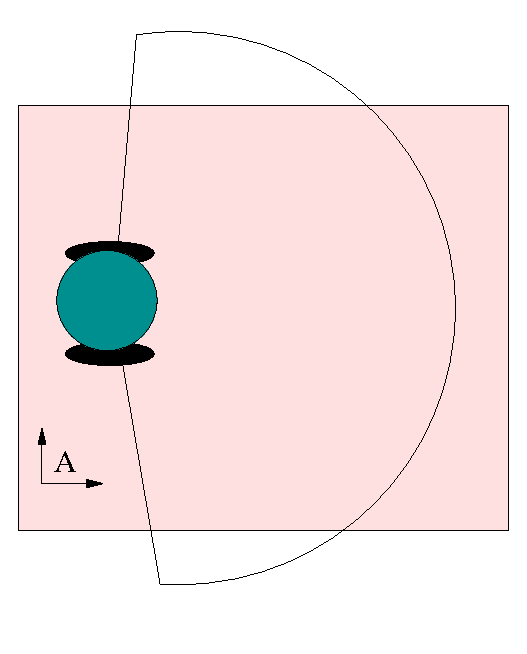
\includegraphics[height=3cm]{Pics/fig_transition1}
\label{fig:StartNewa}
}\quad \quad \quad
\subfigure[Entering Unexplored Area (region {\bf B})]{
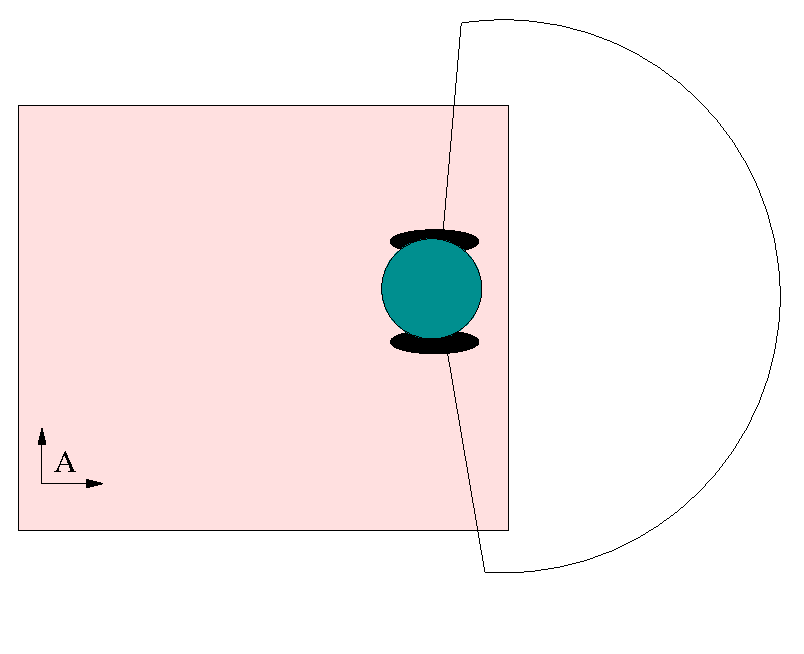
\includegraphics[height=3cm]{Pics/fig_transition2}
\label{fig:StartNewb}
}\quad
\subfigure[Coming Back to region {\bf A}]{
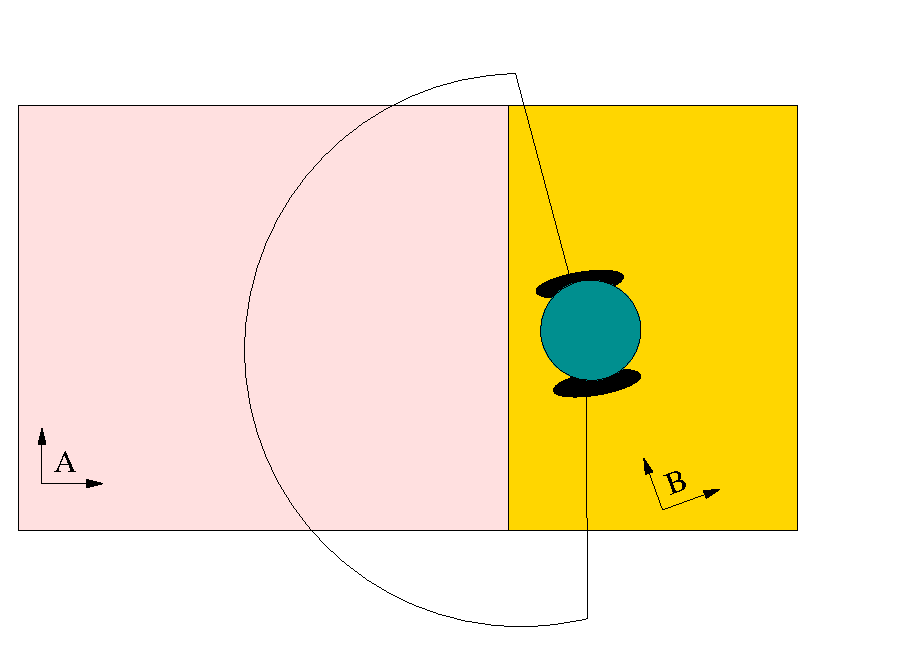
\includegraphics[height=3cm]{Pics/fig_transition3}
\label{fig:StartNewc}
}
\end{center}
\caption{The overlap between the sensor range and the area of the local 
         map is used to decide when to start a new map or transfer to a 
         neighbouring region.}
\label{fig:StartNew}
\end{figure}

The robot constantly checks how much of its' sensor field of view
falls within the current region (see \refFigure{fig:StartNew}), and
how much falls in the neighbouring regions. When the robot detects
that one of the neighbouring regions has a significantly larger
overlap with the sensor field of view than all the others, it switches
to that region. The goal is to maximise the proportion of observations
that match to an existing map. If one assumes uniform distribution of
landmarks in the environment and uniform detection rates for a sensor
view (i.e. landmark straight ahead is as easily detectable as the one
on the robots left), than this approach actually maximises the number
of re-observed landmarks. In the real world landmarks are not
distributed uniformly, and the detection rates for different views of
a landmark are different. This approach nevertheless provides a good,
computational inexpensive measure for determining map transitions.

A sensor view based approach also makes the decision to start a new
map trivial. If no region overlaps sufficiently with the sensor field
of view, the robot assumes it is entering an unexplored area and
initiates a new map. In order to avoid oscillations between two
regions when the robot is near the boundary, thresholds are set to
slightly favour staying in the current region.


\section{Starting a New Local Map}
\label{sec:starting_new_map}
%How it is done.
%\begin{enumerate}
%\item Finalise current map.
%\item Add new node and link to the map graph.
%\item Initialise particles - empty map, 0 pose.
%\item Compute initial area.
%\item Subtract ``neighbours''.
%\end{enumerate}


A pose of a robot is represented by a set of particles: at any time
instant HTSLAM maintains a set of path particles, and the
corresponding maps conditioned on the path. When a new map is started
the relative pose of the current and the new map reference frames is
different for every particle. Since the pose of the robot in the new
map is known exactly (and so is equal for every particle), it is
possible to compute the relative transformation between the two maps
for every particle. Effectively, a set of particles is a sample from
the distribution $\prob{\tr{}{A}{B},\mapA}$.  The new empty map that
is created is independent of the previous path of the robot, hence

$$
 \prob{\mapA,\tr{}{A}{B},\mapB} = \prob{\mapA,\tr{}{A}{B}}\prob{\mapB}.
$$

Furthermore, tuple $(\mapA, \tr{}{A}{B})$ is actually a single variable.
Since the map is conditioned on the path of the particle, there exists a
one to one non-random relationship between the transition and map $A$,
that is $\tr{}{A}{B} = f(\mapA)$. Therefore

$$
\prob{\mapA,\tr{}{A}{B},\mapB} \equiv \prob{\mapA,\mapB}.
$$

At the time when \mapB is started $\prob{\mapA,\mapB}$ is assumed to
be a discrete uniform distribution. Any pair of map instances from
\mapA and \mapB is considered to be equally likely\SILENT{need to be
  more clear that any SAMPLE from A,B is equally likely}. This is due
to the fact that \mapB is empty, and so any sample from \mapB is
equally ``compatible'' with any sample from \mapA. As \mapB is
explored, more information becomes available that can be used to
evaluate the relative compatibility of the $(\mapA,\mapB)$ sample. For
example if a set of landmarks appears in both \mapA and \mapB, and
their correspondence is known, one can evaluate the likelihood of the
map pair using covariance intersection \cite{cov_intersection}
of the common landmarks. If the maps contain some sort of free space
information, it can also be used to measure compatibility. However
there is no need to continuously update the transition distribution;
it is assumed to be unchanged until it is time to sample from it. The
only information that needs to be stored at the time of creating a
transition is a mapping $\mapA \Rightarrow \tr{}{A}{B}$.

%\NOTE{Rewrite in bullet form}
A new node is added to the graph, this node is connected to the
current map.  The current reference frame is set to that of a new
node. The initial map region is computed and assigned to the new
map. All the neighbouring regions are then projected into the new
coordinate frame and are subtracted from the initial map region to
force the non-overlapping constraint. A pose of all particles is then
set to some initial value, their maps are set to empty, and the
mapping process is restarted.

As the robot continues mapping new region, any error in the map and robot
pose estimate remains conditionally independent from errors in any
previous maps. This independence remains until the region is
revisited.


\section{Switching Maps - Revisiting}
\label{sec:revisiting}
%\begin{itemize}
%   \item How we decide to transfer to a different map.
%   \item What happens when we do.
%   \item Describe difference between traversing the link first
%        time and thereafter.
%\end{itemize}

When the robot detects that there is a significant overlap between one
of the neighbouring regions and the sensor field of view, it switches
to the corresponding local map. Most of the time, the neighbouring
region will be adjacent to the current region, however two regions
that are separated by several links in the graph can also be
considered neighbours if the compound coordinate transformation from
one to another is sufficiently certain.  In the case when the regions
are not directly connected, the transition is performed along the
shortest path between the two regions and is equivalent to performing
several transitions one after another. The procedure for computing the
shortest path between two local maps is discussed in the chapter on
loop closing (chapter~\ref{chpt:LoopClosing}).

Consider the transition under the assumption that the two regions are
adjacent. For clarity let $A$ be the region that was mapped first, and
$B$ the region created subsequently. As described previously
(chapter~\ref{chpt:MapStructure}), each transition maintains joint
probabilities that capture the three-way relationship of the two maps
joined by the transition and their relative pose. It is therefore
possible to sample a map-transition-map triple $\{
{\mapA,\tr{}{A}{B},\mapB} \} \sim \prob{\mapA,\tr{}{A}{B},\mapB} $.
 

\begin{figure}
\begin{center}
\subfigure[Path in region {\bf A}.]{
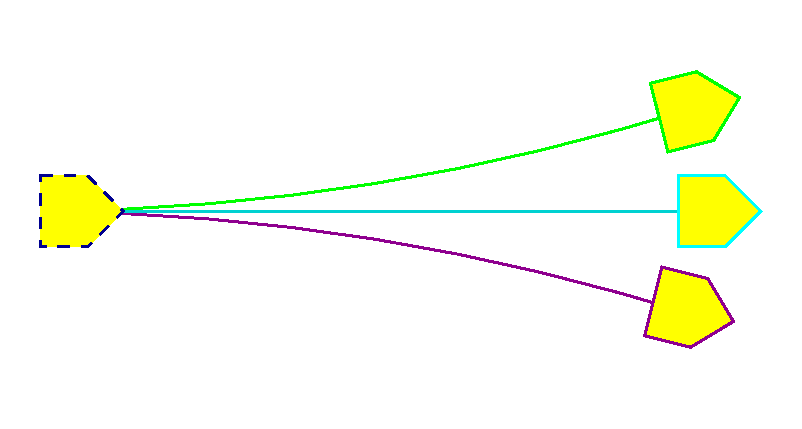
\includegraphics[height=2cm]{Pics/fig_revisit1}
\label{fig:MappingExampleA}
 }
 \subfigure[Path in region {\bf B}.]{
 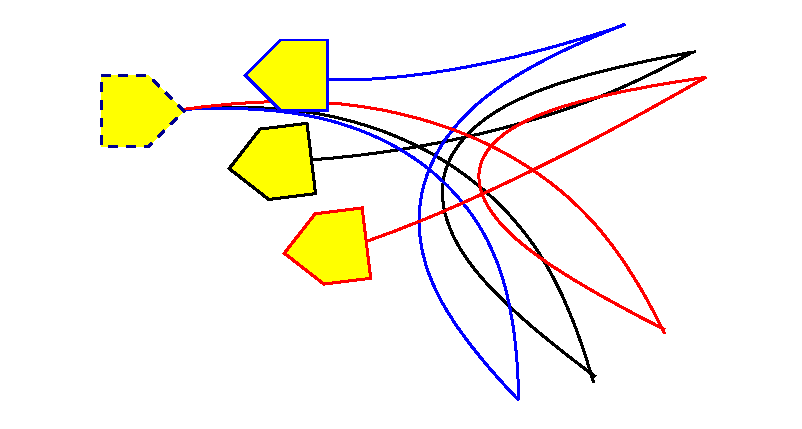
\includegraphics[height=2cm]{Pics/fig_revisit2}
 \label{fig:MappingExampleB}
 }\\
 \subfigure[Combined paths.]{
 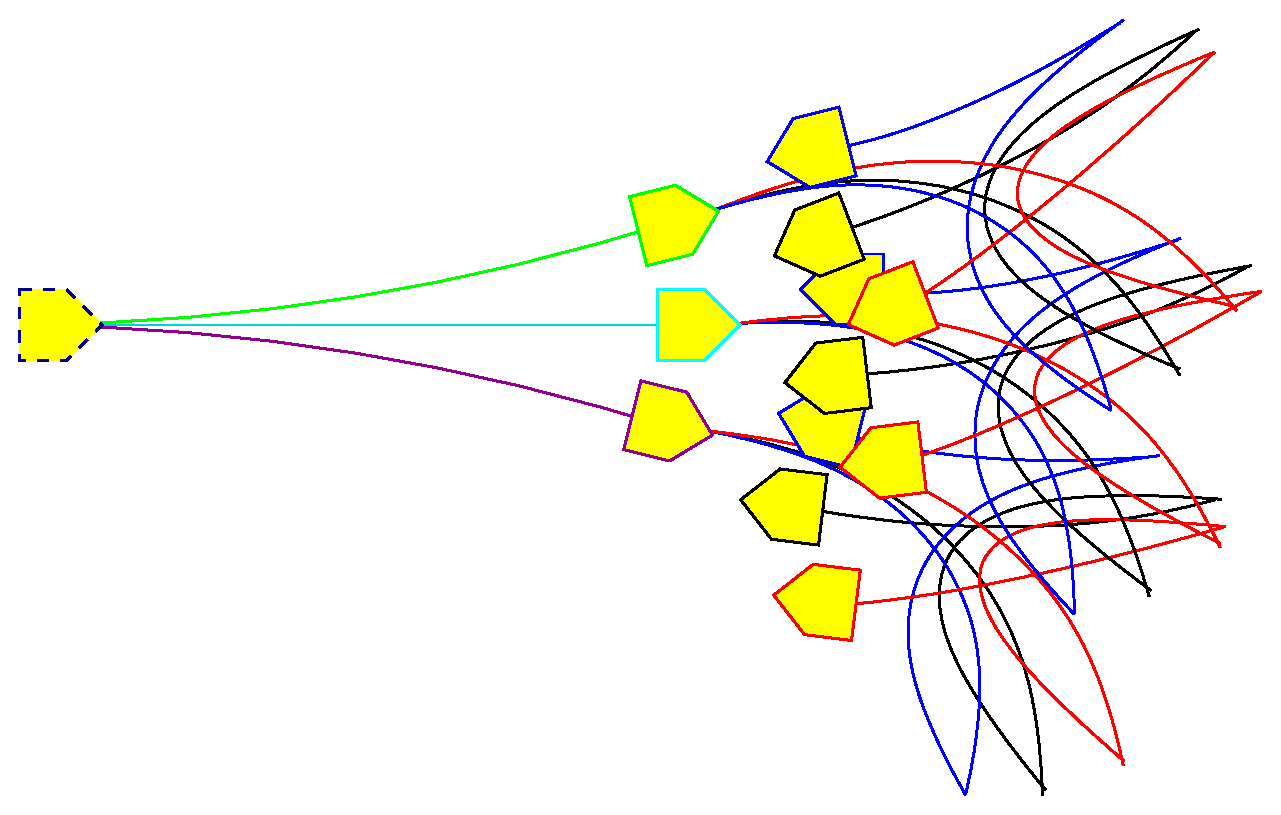
\includegraphics[width=6cm]{Pics/fig_revisit3}
 \label{fig:MappingExampleC}
 }
 \subfigure[Sampled paths.]{
 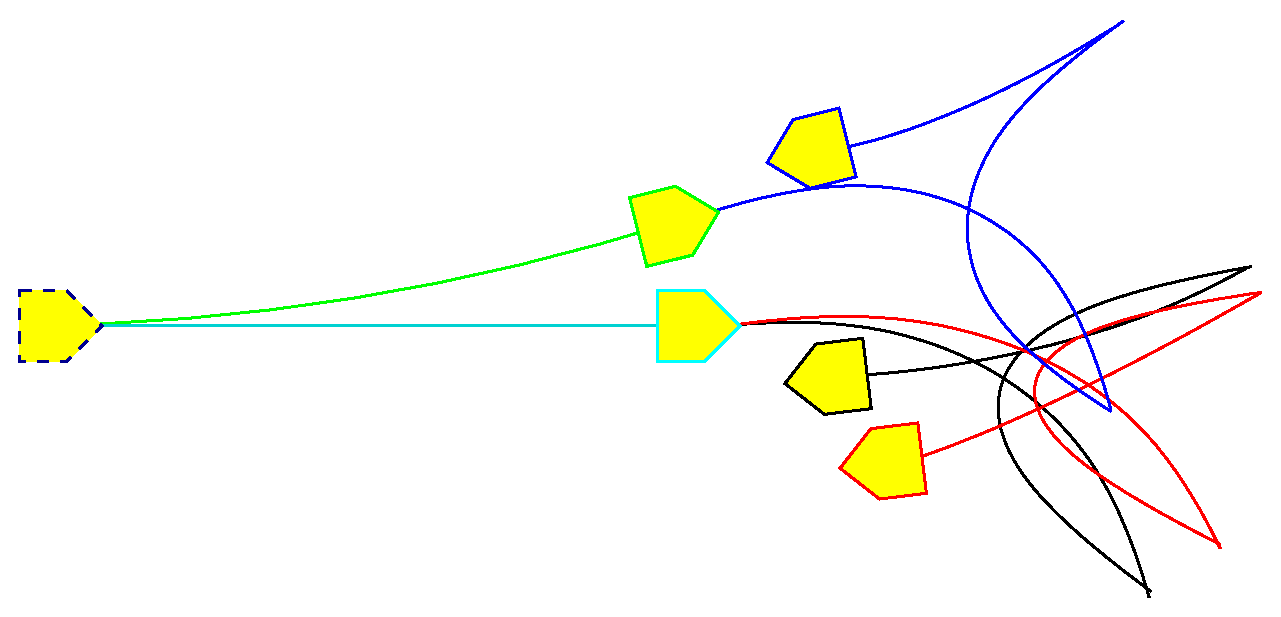
\includegraphics[width=6cm]{Pics/fig_revisit4}
 \label{fig:MappingExampleD}
 }
 \end{center}
 \caption{Example: revisiting map region.}
 \label{fig:MappingExample}
\end{figure}



It is best to describe the process of transition from one map to
another with an example, referring to
\refFigure{fig:MappingExample}. The robot has a car like driving
system and lives on a plane. Three particles are used to approximate
robots motion. The robot starts in region $A$ and travels some
distance forward, taking observations. Some time later the robot
reaches the boundary of region $A$ and starts a new map $B$. Again
three particles are used to model the uncertainty of the robot's path
in map $B$. After performing a three point turn the robot returns to
region $A$. At this point there are 9 possible paths the robot could
have taken. These paths are illustrated in
\refFigure{fig:MappingExampleC}. By starting a new map $B$, HTSLAM
effectively conserved the uncertainty at that time instant. Now, when
the robot is returning to the region $A$ there are more possible paths
to consider. More hypothesis are beneficial. The number of hypothesis
is akin of resolution in images - more hypothesis provide a clearer
picture of the observed uncertainty. HTSLAM used only 3 particles for
mapping but has 9 possible paths. A global mapping approach would have
had to use 9 particles (that is $N^2$) to get the same ``resolution''
on the uncertainty. While having higher resolution is desirable,
computational resources are limited. Therefore in this example only 3
paths have to be sampled.

One can assume that all paths are equally likely and sample
appropriately. This approach is, however, wasteful. If the two maps
share common landmarks, it should be possible to evaluate each path
based on some map overlap criteria that approximate
$\prob{\mapA,\mapB}$.

Alternatively one can use some form of adaptive particle filter
\cite{KLDSampling} that adjusts the number of particles
based on the spatial uncertainty of the robot's pose. In the case of a
transition from one map to another, the uncertainty of the robot's
location increases and hence the number of particles would be
temporarily increased. After some observations of map $A$, bad paths
would be pruned out through the process of re-sampling. 

%% \NOTE{I reckon
%% this approach is a better one. It is however not very clear, what will
%% happen when running multiple hypothesis (loop closing). I know it have
%% been done for localisation, but can't find any references for SLAM.}

Once the robot transferred from $B$ to $A$ the two maps are no longer
independent. Any further update to map $A$ will depend on the pose of
the robot in map $A$, robot pose in map $A$ depends on the transition
and on the robot pose in map $B$ at the time of transition, robot pose
in map $B$ at the time of transition in turn depends on the map
$B$. Therefore all three variables, map $A$ and $B$ and the transition
between them are now dependent variables. This dependency is
represented in the HTSLAM structure by a sample from the
$\prob{\mapA,\tr{}{A}{B},\mapB}$.

In practice this means that each particle now knows which map to
update in $A$ and in $B$, and which transition to use when
transferring from one to the other \SILENT{need to be more clear about
the samples from map A,B}. From that point onwards no sampling will be required
when transferring from $A$ to $B$ and back. If the robot continues
operating only within these two maps, the mapping process will be
equivalent to a normal FastSLAM, except that the environment is split
into regions of bounded size, and hence computation requirements are
bounded.

Due to the process of re-sampling, the overall uncertainty in the
transition between maps $A$ and $B$ will decrease over time, as more
observations become available. This is due to the fact that particles
that ended up with ``bad'' transition hypotheses won't match
observations to the map as well as the ones with ``good'' transition
hypotheses, and will be pruned out during the re-sampling stages of
the particle filter. While this is generally a good thing, there is a
drawback: particle deprivation problem. Since there is no process in
place that will introduce new particles to the transition, over time
the transition estimate will collapse to just a few or even one
particle. 

%\NOTE{Why is it a problem, when is it not a problem. What
%can be done about it. }

If the robot starts a new region $C$ and then returns to
region $A$, a similar process of sampling will occur. This time,
however, every map in $A$ is linked to a map in $B$ and to the
transition between regions $A$ and $B$.


% LocalWords:  FastSLAM Montemerlo Thrun Kalman EKF Submap observability endfor
% LocalWords:  Bayes endif odometry ms XR holonomic Nieto HTSLAM teleportations
% LocalWords:  teleportation Rao Blackwellised


\chapter{Multiple Hypothesis and Loop Closing}
\label{chpt:LoopClosing}
In this chapter an approach to loop closing is presented.
Section~\ref{sec:loop_detection} describes how loops in the
environment are detected. Map matching is described in
section~\ref{sec:map_matching}. The update to the global structure
needed after loop closing is presented in
section~\ref{sec:global_map_update}. Then
section~\ref{sec:loop_confirm} describes how HTSLAM deals with
multiple hypothesis arising from the loop closing.


\section{Loop Detection}
\label{sec:loop_detection}

%% Describe how we decide to try map matching. Use of map regions in the
%% probabilistic framework. Why is it great.

%Even though there is no global
%reference frame in the HTSLAM structure, it is possible to obtain an
%estimate of the relative pose of any two regions in the map. Regions
%do not need to be adjacent. The exact mechanism for doing that is
%described in \ref{sec:relative_poses}. It is therefor possible to
%compute the likelihood of the robot being in any of the regions of the
%map at any given time instance.

When mapping new terrain a robot periodically checks whether it has
returned to a region that was mapped previously. Since the HTSLAM
structure does not have a global reference frame, a robot pose is only
defined for the region currently being mapped. It is however possible
to estimate a relative alignment of any two given regions. Using this
information, the robot pose can be transformed from one reference frame
to another. The exact mechanism for doing that is described in
Section~\ref{sec:relative_poses}.

There are three levels of tests for loop detection. Higher level tests
are only considered if all the previous tests have passed.

\begin{itemize}
\item Robot pose: is the robot likely to be within the region?
\item Map similarity (map matching): does the other map look like
the current map?
\item Consistency with current observations: assuming the robot is
  revisiting a region, are the observations consistent with the map of
  that region? (I expect to see a coffee machine around the corner: is
  it there?)
\end{itemize}

%If the likelihood of the robot being in a certain region is relatively
%high we attempt to match maps. If map matching succeeds we align the
%maps, if alignment is compatible with the prior estimate of the
%relative pose we create new hypothesis, later on if the hypothesis
%succeeds over all other hypothesis that might be present at the time,
%we have closed the loop (hooray!). Now a more detailed description of
%how we do each of the steps.

%Provide notation for examples. Assume robot starts in map $A$, goes
%through maps $B,C,D,E$, before establishing correspondence between
%landmarks in maps $A$ and $E$.


\subsection{Computing Relative Map Poses}
\label{sec:relative_poses}

Since HTSLAM maps in general can contain cycles, there might be
multiple paths between any two regions. To resolve this ambiguity the
graph structure of the map is converted into a tree with the root
being the current node. This can be achieved using either breadth-
first traversal of the graph or with Dijkstra's algorithm for finding
the shortest path in the graph \cite{dijkstra_shortest_path}.

\subsubsection{Breadth First Traversal}

\begin{figure}
\begin{center}
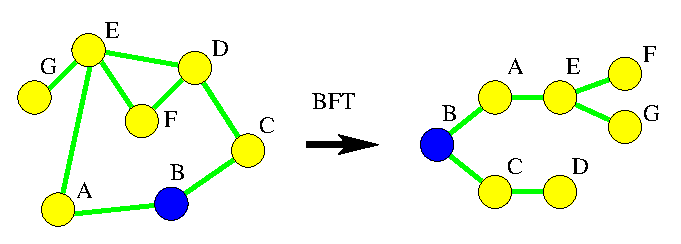
\includegraphics[width=12cm]{Pics/fig_bft}
\end{center}
\caption[Breadth First Traversal]
{Breadth First Traversal is used to find a shortest paths (in
the number of transitions required) from one map frame to all the
other map frames.}
\label{fig:bst}
\end{figure}

One sensible approach is to minimise the number of transitions needed
to compute the relative pose of two map frames. As it happens, it
is possible to compute the shortest path between one of the nodes of
the graph and all the other nodes of the graph by converting a graph
in to a tree using Breadth-First Traversal (see \refFigure{fig:bst}).
The computational complexity of the BFT approach is $O(|V| + |E|)$,
where $|V|$ is the number of nodes (vertices) and $|E|$ is the number of
edges in the graph.


\subsubsection{Dijkstra's Shortest Path Algorithm}


Dijkstra's shortest path algorithm computes a path between two nodes
of the graph that minimises some metric. In the case of HTSLAM, it is
desirable to find a path between two regions, that has a most certain
compound transition. To implement this approach one requires an
accurate estimate of the uncertainty of the compound transition.  One
possible solution is to approximate the error in each transition with
a Gaussian. This way compound transitions can be computed
recursively. Dijkstra algorithm can then be modified to minimise the
determinant of the covariance of the compound transition. Similarly to
BFT Dijkstra algorithm generates a tree from the graph. The
computational complexity of Dijkstra's Algorithm is $O(|V| \log |E|)$,
which is higher than that of BFT.

Due to approximation errors, Dijkstra's algorithm might not actually
compute the most certain path. As a result, the benefit of using
Dijkstra's algorithm for this problem is questionable. Experimentation
with vision data (Chapter~\ref{chpt:Vision_Results}) has shown that
the Gaussian approximation for the transition uncertainty can be poor.
An alternative distance metric should be used for the Dijkstra
algorithm, one involving the number of transitions along the path as
well as the estimate of the uncertainty. However no experimentation
with transition uncertainty representation was conducted. In the
experiments presented in this thesis the BFT algorithm was used, and
was proven to be sufficient.


\section{Map Matching}
\label{sec:map_matching}

%\begin{enumerate}
%\item Problem definition: search for a maxima in the landmark
%   correspondence space. Evaluation criteria is defined by the edge
%   matches.  
%\item Problem is equivalent to finding a branch in a decision tree with
%   the highest score.
%\item Depth first brute force approach is impractical. Order N factorial.
%\item Early exit criteria are used : no need to process all
%   branches. Two categories: spatial compatibility + maximum
%   achievable score.
%\item Preprocessing steps allow to traverse good branches first, that
%   makes early exit more efficient.
%\end{enumerate}

Given two local maps, a method is required to assess the probability
that they correspond to the same region in the environment and find
their relative alignment. The choice of map matching algorithm depends
on the type of local mapping module. This thesis deals with feature
based maps (other types include: occupancy grids, dense point clouds and
laser scans). In the case of feature based maps, the map correspondence
problem is split into a number of landmark correspondence problems. To
solve the map correspondence problem, one needs to find the most likely
set of common landmarks between the two local maps. It is a requirement
of HTSLAM that the correspondence problem can be solved without accurate
knowledge of the relative map alignment. The nearest neighbour gating
technique, commonly used for data association problems, will not work in
this situation since the uncertainty in the relative alignment of the
two maps is large. There are a number of batch data association
techniques. One of them is the joint probability branch and bound(JPBB)
\cite{neira01:_data_assoc_stoch_mappin_using} method, which is more
robust to pose uncertainty, than nearest neighbour, however it still
assumes that the rough alignment is known. JPBB performs a search in a
correspondence decision tree for a branch with the best match.

Another batch data association technique is the graph theoretic
approach \cite{tardos02:_mappin_local_indoor_envir_using_sonar_data}.
Essentially this algorithm performs a search for a clique (the largest
fully connected sub-graph of a graph) in a sparse correspondence graph.
The correspondence graph is constructed from the geometric feature
matches (distances between landmarks, in the case of point landmarks).
If individual landmarks can be differentiated in some way (for example
a door landmark cannot match a chair landmark, or a pink door cannot match
a green door), such a constraint is referred to as an {\it absolute}
constraint. Absolute constraints are also taken into account when
constructing the correspondence graph. Unlike JPBB, the graph based
approach can work without prior knowledge of the relative alignments
of the two sets being matched: however if a prior is available it is
used.

Both of the batch methods mentioned above were developed for data
association in EKF SLAM. As a result they assume that a set of
uncorrelated observations is matched to a set of correlated
landmarks. However they can be easily extended to match two sets of
landmarks instead. In HTSLAM landmarks are uncorrelated, and so some
computation can be simplified significantly.

The approach used in this thesis is similar to the graph approach.
Like the graph approach it looks for a maximum clique of the
correspondence graph, but without constructing the graph explicitly.
This approach computes joint compatibility in a slightly different
way. Geometric and absolute constraints are used as in the graph
approach, but in addition this approach also exploits constraints
arising from the alignment of the two sets. Generally, geometric
constraints alone are not sufficient to disregard all impossible sets
of correspondences. Any two sets of landmarks which are mirror images
of one another will satisfy the geometric constraints, but the
landmarks in these sets do not correspond (see
\refFigure{fig:mirror_sets}).

\begin{figure}[htbp]
  \centering
  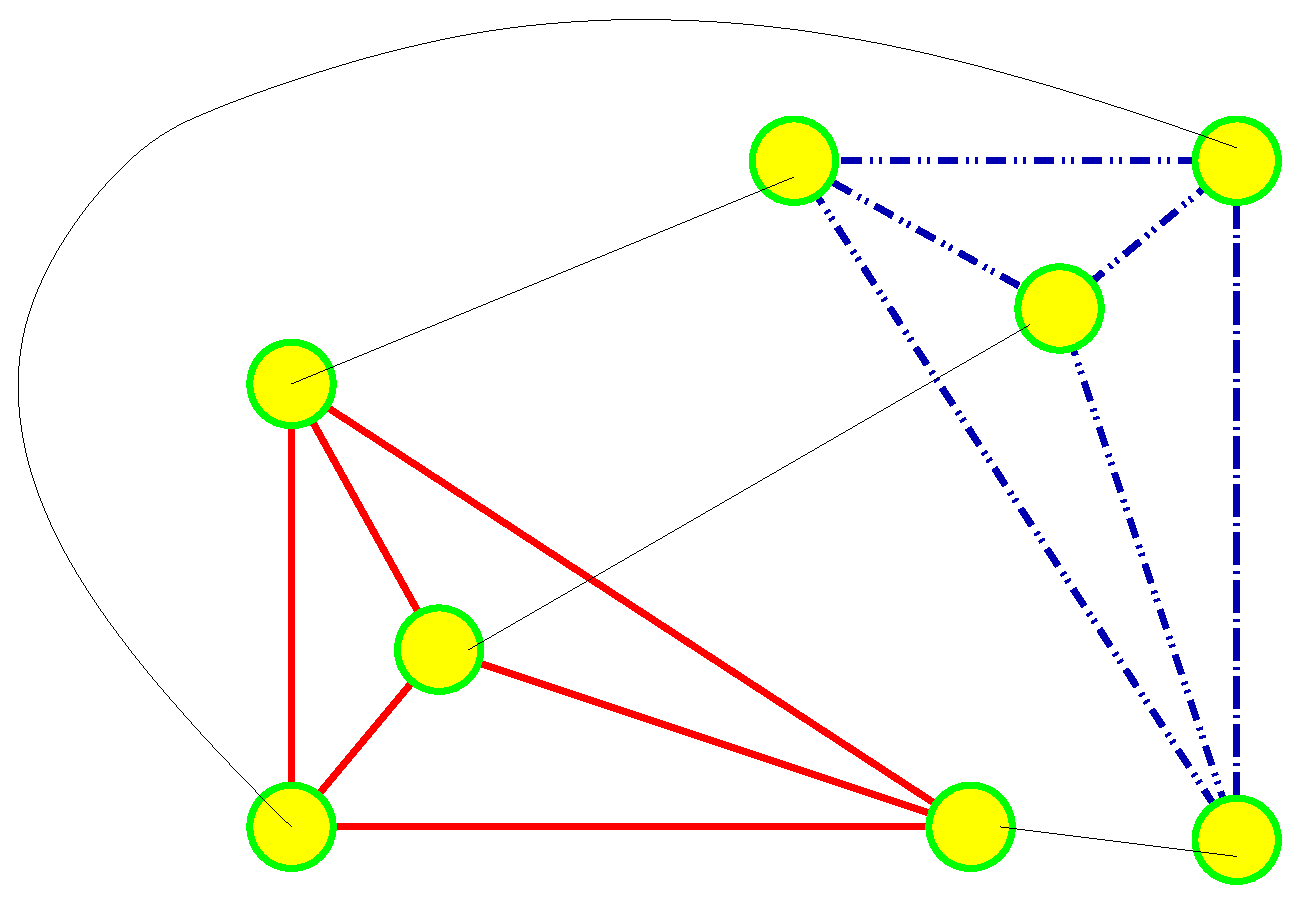
\includegraphics[width=6cm]{Pics/fig_mirror_sets}
  \caption[Reflection and alignment]{Two incompatible landmark sets, that {\bf do} satisfy
    geometric constraints. One set is a mirror image of another, the
    distances between landmarks match, but the sets cannot be aligned
    by a Euclidean transform.
}
  \label{fig:mirror_sets}
\end{figure}

%TODO: Need a tighter integration with the rest of the text.
The most direct way to evaluate a correspondence hypothesis is to
perform a two-view reconstruction of the scene, and then compute the
likelihood of the reconstruction. Let $\theta_i$ be a landmark
pose in the reference frame of map $a$, let $\theta_i^a, \theta_i^b$
be an estimate of the landmark $i$ in the reference frames $a$ and
$b$ respectively. Let ${\bf R},{\bf t}$ be a rotation and translation
from frame $a$ to frame $b$. Assume also that a prior $p\left({\bf
R},{\bf t}\right)$ is available. The reconstruction process needs to
find $\left[\theta_1,...\theta_n, {\bf R},{\bf t}\right]$ that
maximises
\begin{equation}
p\left({\bf R},{\bf t}\right)
\prod_{i}^n p\left(\theta_i | \theta_i^a\right)
p\left({\bf R}\theta_i + {\bf t} | \theta_i^b\right).
\label{eqn:align}
\end{equation}

The maximum of \refEquation{eqn:align} can be used as a measure of
the likelihood of a particular landmark correspondence configuration.
While there is no closed form solution to this problem, an iterative
numerical optimisation can be used to find the maximum of
\refEquation{eqn:align}. This process is outlined in
Section~\ref{sec:map_alignment}. Such an operation is computationally
expensive and cannot be used to search for the most likely
configuration. However it can be applied to compare the best few
hypotheses.



Preprocessing step: let $E^a_{i,k}$ be the edge between landmarks $i$
and $k$ in the map $a$. For every landmark correspondence compute an
upper bound on the size of the correspondence set it can belong to
$$
u_{ij} = \sum_{k \ne i} \sum_{l \ne j} {\bf MATCH}(E^a_{i,k}, E^b_{j,l}).
$$

Here function ${\bf MATCH}$ returns 1 if edges match and zero
otherwise. Edges match if the landmarks on either side of the edge
satisfy absolute constraints {\bf AND} their lengths are sufficiently
similar {\bf AND} the alignment arising from the edge correspondences
is consistent with the prior. When implemented naively the
computational complexity of the preprocessing step is $O(N_eM_e)$,
where $N_e,M_e$ are number of edges in the two sets. However, if one
first sorts the edges by their lengths, one does not need to match
each edge to every other. The complexity in that case will be
$O(N_e\log N_e + M_e\log M_e + N_eK)$ where $K \leq M_e$ but in
practice $K \ll M_e$ typically, and depends on the search window width and the
distribution of edge lengths.

Let $S$ be a set of landmark correspondence hypotheses. Each element
of $S$ is a triple $(u_{ij}, i, j)$, where $u_{ij},i,j$ mean the same
as above. Set $S$ is sorted in descending order according to
$u_{ij}$. Let $M$ be a set of jointly compatible
correspondences. $P_{ab}$ is a prior on relative alignment of the two
sets being matched. ${\bf MATCH}$ is a lookup table: inputs are edges
from map $a$ and map $b$, and the output is a boolean indicating
whether the two edges match. $M_{max}$ is a set of all current best
matches. Matches with equal number of common landmarks are considered
equally likely. $N_{max}$ is a number of common landmarks in the
current best match or matches. $T^a,T^b$ are boolean arrays indicating
which landmarks from $a$ and $b$ respectively, have been matched.

The proposed matching algorithm is recursive. The level of recursion
is limited by the number of landmarks in the smaller of the two
maps. The algorithm is presented in pseudo-code.

%Algorithm in the pseudo-code.
\begin{pseudocode}{MatchMaps}{L_a, L_b, P_{ab}}
 \COMMENT{$L_a,L_b$ set of landmarks to be matched}\\
 \COMMENT{$P_{ab}$ prior on relative alignment}\\
 \GLOBAL{E^a,E^b,{\bf MATCH},S}\\
 \GLOBAL{M_{max},N_{max},T_a,T_b}\\
\\
 E^a = \CALL{ComputeEdges}{L_a}\\
 E^b = \CALL{ComputeEdges}{L_b}\\
 (S,{\bf MATCH}) = \CALL{MatchEdges}{E^a,E^b,P_{ab}}\\

 N_{max} = 3 \quad \COMMENT{At least three landmarks have to match.} \\
 M_{max} = \{\}\\
 T_a = [\FALSE,\FALSE,\cdots,\FALSE]\\
 T_b = [\FALSE,\FALSE,\cdots,\FALSE]\\

 \CALL{RecursiveSearch}{S,\{\},P_{ab}}\\

 \RETURN{ M_{max}}
\end{pseudocode}

\begin{pseudocode}{RecursiveSearch}{S,M,P_0}
 \GLOBAL{M_{max},N_{max},T_a,T_b}\\
 \\
 \IF size(M) > N_{max}\THEN
 \BEGIN
     M_{max} = \left\{ M \right\}\\
     N_{max} = size(M)
 \END
 \ELSEIF size(M) = N_{max}
 \BEGIN
     M \rightarrow M_{max}
 \END\\
 \\
 \WHILE size(S) + size(M) \ge N_{max} \AND S \ne \left\{\right\} \DO
 \BEGIN
      \left(u_{ij},i,j\right) \leftarrow S \\
      \IF u_{ij} < N_{max} \THEN
      \BEGIN
         \RETURN{}
      \END
\\
      \IF \CALL{IsCompatible}{i,j,M,P_0} \THEN
      \BEGIN
         (i,j) \rightarrow M \\
         T_a[i] = T_b[j] = \TRUE\\
         P = \CALL{UpdateAlignment}{M,P_0}\\
         \CALL{RecursiveSearch}{S,M,P}\\
         (i,j) \leftarrow M\\
         T_a[i] = T_b[j] = \FALSE\\
      \END
 \END
\end{pseudocode}

\begin{pseudocode}{IsCompatible}{i,j,M,P}
  \GLOBAL{T_a,T_b,{\bf MATCH},E_a,E_b}\\
  \\
  {\bf r} = \NOT \left( T_a\left[i\right] \OR T_b\left[j\right] \right)\\

  \WHILE {\bf r} \AND M \ne \left\{\right\} \DO
  \BEGIN
     (k,l) \leftarrow M\\
     \IF {\bf MATCH}\left[E^a_{i,k}, E^b_{j,l}\right] = \TRUE \THEN
     \BEGIN
        A = \CALL{RotationFromEdges}{E^a_{i,k}, E^b_{j,l}}\\
        {\bf r} = \CALL{CompatibleRotation}{A,P}
     \END\\
     \ELSE \BEGIN
        {\bf r} = \FALSE
     \END\\
  \END\\
  \RETURN {\bf r}

\end{pseudocode}


\subsubsection{Distance Between Landmarks}

The distance between two landmarks is not known exactly, and the
uncertainty is a non-Gaussian distribution. It is approximated by a
Gaussian using first order Taylor series expansion. An alternative is to
use an unscented transform \cite{unscented}. The unscented transform
provides a more accurate estimate, with similar computation
requirements. In this work however, Taylor series approximation was
used.

The mean and variance of the distance is computed according to the
following approximation:

\begin{eqnarray}
  \mu_d  &=& f([x_1,y_1,x_2,y_2]^T) = \sqrt{(x_1-x_2)^2 + (y_1-y_2)^2}
\label{eqn:dist_estimate_mu}\\
 \sigma_{d}^2 &=& \bigtriangledown f \left [\begin {array}{cc} \Sigma_1 & 0\\
 0& \Sigma_2 \end{array}\right ] \bigtriangledown f^T.
\label{eqn:dist_estimate_cov}
\end{eqnarray}

Here $\bigtriangledown f$ is a Jacobian of $f$, evaluated at
$[x_1,y_1,x_2,y_2]^T$. $\Sigma_1$ and $\Sigma_2$ are the two landmark
covariances. Equations \refEquation{eqn:dist_estimate_mu} and
\refEquation{eqn:dist_estimate_cov} can be simplified by introducing
variables $\Delta x = x_1 - x_2$, and $\Delta y = y_1 - y_2$, the
uncertainty of $\Vector{\Delta x\\ \Delta y}$is equal to a sum of
uncertainties of the two landmarks $\Sigma_\Delta = \Sigma_1 +
\Sigma_2$:
\begin{eqnarray}
\mu_d &=& \sqrt{\Delta x^2 +\Delta y^2}\\
\sigma_d^2 &=& \bigtriangledown f \Sigma_\Delta \bigtriangledown f^T
\end{eqnarray}
where
$$ 
\bigtriangledown f = \left[
\frac{\Delta x}{\sqrt{\Delta x^2 + \Delta y^2}}, 
\frac{\Delta y}{\sqrt{\Delta x^2 + \Delta y^2}}
\right].
$$

%\subsubsection{Using Landmark Appearance for Matching}

The distance between landmarks is not the only transform invariant
feature. It might be possible to differentiate individual landmarks to
some degree. In the case of corner landmarks, for example, a convex
corner should not match a concave corner. Landmark type is therefore
used as a binary measure to disregard impossible landmark
correspondences. In the case of vision landmarks, cross-correlation of
the landmark templates can be used to compute the likelihood of the
two landmarks corresponding.

Using landmark appearance or type is beneficial to the task of map
matching, as it reduces computation time and increases the likelihood
of finding correct correspondences. In the situation when landmarks do
not have any attributes that can be used to differentiate them, any
landmark correspondence is considered to be possible and equally
likely. The proposed algorithm can work without this extra
information, but will use it if it is available.

\subsection{Map Alignment from 2 Landmark Correspondences}

Generally when closing the loop there is a priori knowledge of the
relative alignment of the two maps. No matter how uncertain this
knowledge is, it is still beneficial to use it to speed up the
matching process by disregarding landmark correspondences that are in
disagreement with the prior. In the case of a point landmark, a single
landmark to landmark correspondence does not have a rigid constraint
on the relative map pose, however a pair of point landmark
correspondences is sufficient to compute the relative pose of the two
maps. Since the landmark locations are not known exactly, the relative
pose will also have some uncertainty. This uncertainty, however, is
likely to be significantly less than that of a prior, and is therefore
used to assess the possibility of the correspondence being
correct.

Assume $\theta^a_1$ and $\theta^a_2$ are true poses of the two
landmarks expressed in the reference frame of the map $a$. Assume
${\bf R,t}$ are true rotation and translation from frame $a$ to frame
$b$, such that ${\bf R}\theta_1^a + \bf{t}$ is a landmark pose expressed
in frame $b$. $\theta^a_i, \theta^b_j$ are estimates of the first
landmark in frames $a$ and $b$ respectively, and $\theta^a_k,
\theta^b_l$ are observations of the second. Ideally, relative map
pose and the locations of landmarks have to be computed
simultaneously to find the configuration that maximises
\begin{equation}
p(\theta^a_1, \theta^a_2, {\bf R},{\bf t}|
  \theta^a_i, \theta^b_j, \theta^a_k, \theta^b_l) =
p(\theta^a_1 | \theta^a_i)
p({\bf R}\theta^a_1+{\bf t} | \theta^b_j)
p(\theta^a_2 | \theta^a_k)
p({\bf R}\theta^a_2+{\bf t} | \theta^b_l).
\label{eqn:true_alignment_prob}
\end{equation}

In this thesis an approximation is used instead.
Rotation from frame $a$ to frame $b$ is approximated to be
$$
  \phi^{a \rightarrow b} = \tan^{-1} \frac{\Delta y^a}{ \Delta x^a}
  -\tan^{-1} \frac{\Delta y^b}{ \Delta x^b},
$$
where $[\Delta x^a, \Delta y^a]^T = \theta^a_i - \theta^a_k$ and
$[\Delta x^b, \Delta y^b]^T = \theta^b_j - \theta^b_l$. The
uncertainty of the rotation is approximated using first order Taylor
series expansion. Alternatively one can use unscented transform
\cite{unscented}.

For a fixed rotation, translation between two sets of landmarks is
exactly Gaussian, and can be computed analytically. The exact process
is outlined in Section~\ref{sec:map_alignment} on map alignment .



\subsection{Final Map Alignment}
\label{sec:map_alignment}

After landmark correspondence is established HTSLAM requires an
estimate of the relative alignment of the two maps in a
probabilistic manner in order to model the coordinate transformation
between the two maps. This section describes an approach to map
alignment used in the experiments presented in
chapters~\ref{chpt:Laser_Results} and \ref{chpt:Vision_Results}.

HTSLAM requires a sample from the following distribution
\begin{equation}
p({\bf R},{\bf t}) = \prod_{l=1}^{n} \int
p(\mape{}{a}{l})p(\mape{}{b}{l}|{\bf R},{\bf t})d\mape{}{}{}
\label{eqn:align_w}
\end{equation}
Taking $\log$s of both sides
\begin{equation}
\log p({\bf R},{\bf t}) = \sum_{l=1}^{n} \log \int
p(\mape{}{a}{l})p(\mape{}{b}{l}|{\bf R},{\bf t})d\mape{}{}{}.
\label{eqn:align_log_w}
\end{equation}

Let $\theta_i$ be a true location of the landmark $i$ expressed in the
coordinate frame of map $a$. Let ${\bf R,t}$ be a true rotation and
translation from frame $a$ to $b$, such that ${\bf R}\theta_i + {\bf t}$
is a true location of the landmark $i$ in the reference frame of
$b$. Let $\mapA=[(a_1,A_1),...(a_n,A_n)]$,
$\mapB=[(b_1,B_1),...(b_n,B_n)]$ be a set of common landmarks in the two
maps. The mean of the landmark $i$ is denoted by $a_i$ and $A_i$ is the
inverse of the corresponding covariance. It is required to find ${\bf
R,t},\theta_1, \theta_2 ...\theta_n$ that maximise
\begin{equation}
\begin{array}{ll}
p([\theta_1, ...\theta_n],{\bf R},{\bf t} | \mapA, \mapB) =
 \eta \prod& \exp(-(\theta_i - a_i)^T A_i (\theta_i - a_i)/2)\\
&\exp(-({\bf R}\theta_i + {\bf t} - b_i)^T B_i
({\bf R}\theta_i + {\bf t} - b_i)/2),
\label{eqn:align_w0}
\end{array}
\end{equation}
where $\eta$ is a normalisation constant, independent of ${\bf
R,t},\theta_1, \theta_2 ...\theta_n$. Taking $\log$s: 
\begin{equation}
\begin{array}{l}
\log p([\theta_1, ...\theta_n],{\bf R},{\bf t} | \mapA, \mapB) =\\
\log\eta - 0.5 \left[
\sum_i (\theta_i - a_i)^T A_i (\theta_i - a_i) +
\sum_i ({\bf R}\theta_i + {\bf t} - b_i)^T B_i({\bf R}\theta_i + {\bf t} - b_i)
\right].
\end{array}
\label{eqn:align_log_prob}
\end{equation}

The term that needs to be minimised is
$$
F = \left[ \sum_i (\theta_i - a_i)^T A_i (\theta_i - a_i) +
\sum_i ({\bf R}\theta_i + {\bf t} - b_i)^T B_i ({\bf R}\theta_i + {\bf t} - b_i)
\right]
$$

$F$ can be rewritten in matrix form
$$
F =  {\bf x}^T{\bf Gx} -2{\bf Hx} + {\bf c}
$$
where ${\bf x}^T = [\theta_1^T,...,\theta_n^T, {\bf t}^T]$ and
matrices ${\bf G},{\bf H}$ and scalar ${\bf c}$ are:
\begin{eqnarray}
{\bf G} &=& \left[ \begin{array}{ccccc}
A_1 + {\bf R}^TB_1{\bf R}&
0&\cdots&0&
(B_1{\bf R})^T\\
0&A_2 + {\bf R}^TB_2{\bf R}&&&(B_2{\bf R})^T\\
\vdots & & \ddots & & \vdots\\
0&\cdots&0&
A_n + {\bf R}^TB_n{\bf R}&
(B_n{\bf R})^T\\
B_1{\bf R}&B_2{\bf R}&\cdots&
B_n{\bf R}&
\sum_i B_i
\end{array} \right]\\
{\bf H}  &=& \left[a_1^TA_1+b_1^TB_1{\bf  R},...,
a_n^TA_n+b_n^TB_n{\bf R},
\sum_i b_i^TB_i
 \right].\\
{\bf c} &=& \sum_i a_i^TA_ia_i + \sum_i b_i^TB_ib_i
\end{eqnarray}

Note that matrices $A_i,B_i$ are symmetric and hence ${\bf G}$ is a
symmetric matrix as well.

For a fixed rotation, a configuration that minimises $F$ is found by
solving
$$
2{\bf x}^T{\bf G} - 2{\bf H} = 0.
$$

Which is equivalent (${\bf G}$ is symmetric, ${\bf G} = {\bf G}^T$) to
solving
$$
 {\bf Gx} = {\bf H}^T.
$$

Due to the structure of matrix ${\bf G}$, ${\bf x}$ can be solved for
by back-substitution. First, define
\begin{equation}
\begin{array}{rcl}
M_i &=& A_i + {\bf R}^TB_i{\bf R}\\
Y_i &=& B_i{\bf R}\\
S   &=& \sum_i B_i \\
K_i &=& \left[a_i^TA_i + b_i^TB_i{\bf R}\right]^T\\
W   &=& \left[ \sum_i b_i^TB_i \right]^T
\end{array}
\end{equation}

The problem can then be rewritten as a series of linear equations
\begin{equation}
\begin{array}{rcr}
M_1\theta_1 + Y_1^T{\bf t} &=& K_1\\
M_2\theta_2 + Y_2^T{\bf t} &=& K_2\\
&\vdots&\\
M_n\theta_n + Y_n^T{\bf t} &=& K_n\\
\sum_i Y_i\theta_i + S{\bf t} &=& W.
\end{array}
\label{eqn:hjhjk}
\end{equation}

Expressing $\theta_i$ in terms of ${\bf t}$, substituting it in to
(\ref{eqn:hjhjk}), after some rearranging 
\begin{eqnarray}
\theta_i &=& M_i^{-1}K_i - M_i^{-1}Y_i^T{\bf t}\\
{\bf t} &=& \left( S -\sum_i^n Y_iM_i^{-1}Y_i^T \right)^{-1}
\left(W - \sum_i Y_iM_i^{-1}K_i \right).
\end{eqnarray}

Having solved for ${\bf t}$, it is possible to back-substitute to
solve for every landmark location as well. Denoting the solution as
${\bf \mu}$, ${\bf H}={\bf \mu}^T{\bf G}$. $F$ can then be rewritten
as
\begin{equation}
\begin{array}{rcr}
F &=& {\bf x}^T{\bf Gx} - 2{\bf \mu}^T{\bf Gx} + {\bf c}\\
 &=& \left({\bf x - \mu}\right)^T{\bf G}\left( {\bf x - \mu} \right) -
{\bf \mu}^T{\bf G\mu} + {\bf c}.
\end{array}
\end{equation}

For a fixed rotation ${\bf R}$ 
$$
\log p\left(\left[\theta_1, ...\theta_n,{\bf t} \right]^T | 
\mapA, \mapB,{\bf R} \right) =
\log \eta -0.5\left({\bf x - \mu}\right)^T{\bf G}\left( {\bf x - \mu} \right) +
0.5{\bf \mu}^T{\bf G\mu} -0.5 {\bf c}.
$$

From this it follows that under a fixed rotation the error in
translation and landmark locations is a scaled Gaussian
$$
p\left(\left[\theta_1, ...\theta_n,{\bf t}\right]^T | 
\mapA,\mapB,{\bf R}\right) 
= \alpha N({\bf \mu}, {\bf G}^{-1})
$$

The rotation that maximises $\mu^t{\bf G}\mu$ is the most likely
rotation and can be found numerically, for example using Golden Ratio
search for minima algorithm \cite{Pres92}.

Rather than using one optimal value to describe the relative poses of
the two maps, HTSLAM needs a sample of the poses instead. A direct
sample of $({\bf R,t})$ pairs from the distribution given in
\refEquation{eqn:align_w0} is not possible. Since it is possible to find
rotation independent of translation, it is possible to sample rotation
first, and then sample translation condition on a given rotation. For a
given ${\bf R}$, ${\bf t}$ is distributed normally $N(\mu, {\bf
G}^{-1})$.


\section{Augmenting Global Map Structure}
\label{sec:global_map_update}

Assume for the moment a simple scenario: a robot starts in
region $A$, explores new regions $B,C,D,E$, in that order, then
discovers that region $A$ and $E$ overlap.

From landmark correspondences it is possible to infer the relative
pose of the two maps, allowing for an update of the global map
structure. Map alignment is used to compute a new link between the
two maps. The robot then transfers into map $A$ and continues
mapping.  However, this new information also provides information
about the path of the robot along the loop. Before map matching all
paths are equally likely (by construction), subsequently the robot
re-localises itself in map $A$.

If there are no loops in the HTSLAM structure, transitions are
independent variables. This follows from the process by which
transitions are constructed.  However, when the loop is closed one can
no longer think of transitions as independent. New evidence provides
the means to evaluate the joint probability of all transitions along
the path, and this joint probability is generally not equal to the
product of individual probabilities, invalidating the independence
hypothesis.

The big question is whether the fact of loop closing provides
information about the path along the loop. Is there enough information
to evaluate the joint probability of the transitions along the
path? Model approximations introduce errors that accumulate and
introduce biases in the robot pose estimate.

\begin{figure}[htbp]
  \centering

\subfigure[Real path of the robot.]{
  \includegraphics[width=7cm]{Pics/hump}
}
\subfigure[2-d estimate of the path ($A$ and $A'$ should be the same point)]{
  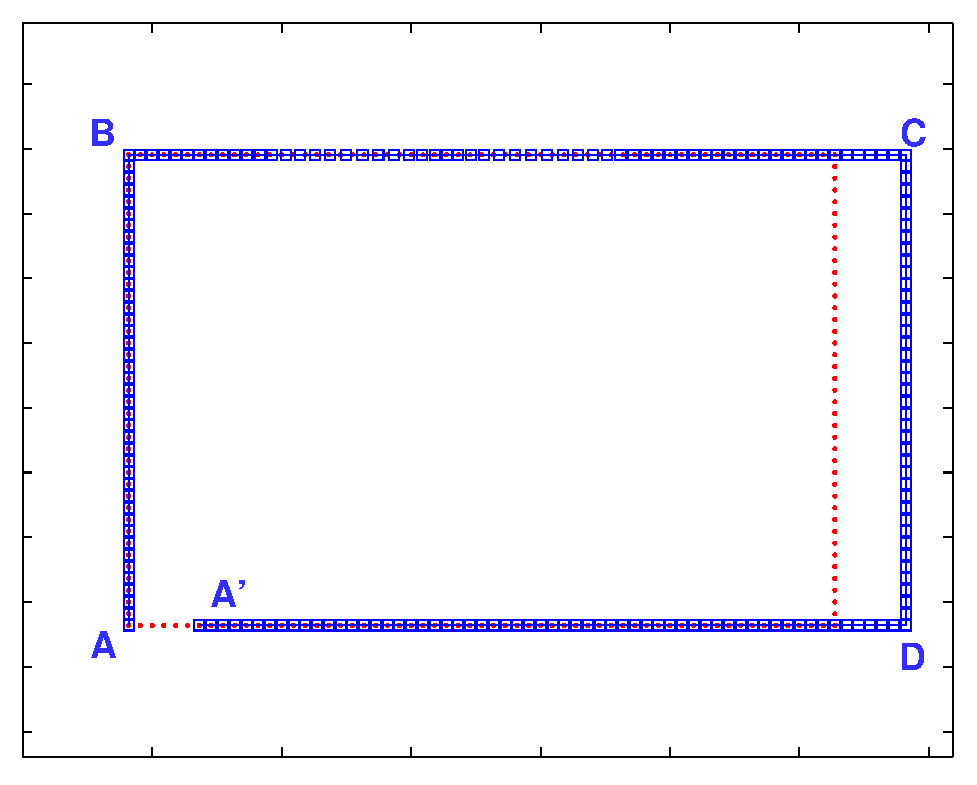
\includegraphics[width=5cm]{Pics/hump_xy}
}
\caption[Effect of unmodelled environment features on localisation]
{Robot starts at point $A$, and travels on a loop
$ABCDA$. Since the segment $BC$ passes over the hill, its length
is longer than that of $DA$. As a result, the flattened path does not
close the loop. By the time robot returns to point $A$, it
estimates its position to be at $A'$.}
  \label{fig:hump}
\end{figure}


The effects of model approximation errors can be significant, as
\refFigure{fig:hump} illustrates. In this example the robot assumes a
planar surface; while this assumption might work well enough for local
observations, it breaks globally. The more accurate the robot's
sensors are, the more obvious model errors become. If your
observations tell you that to get from $A$ to $C$ you either go 100 km
north, then 30 km west, OR 30 km west then 110 km north, then maybe
both these observations are right, but your assumption of a planar
surface is wrong.

If one assumes that the impact of model approximation errors is
insignificant along the path, one can attempt to incorporate all
information along the path when closing the loop. This is however
problematic due to practical considerations. Given there are $K$
transitions along the loop, and there are $N$ particles per
transition, the joint distribution of transitions will be a
$K$-dimensional lookup table, and will contain $N^K$ elements. A
direct computation of joint distribution is clearly not possible.

Traditional metric mapping techniques make an assumption that it is
possible to obtain an exact map of the environment, given an infinite
number of observations. They assume that all dimensions of the problem
are observable. Quite often this is not the case, as was illustrated in
the example above. The limitations of the perception system of an entity
can indeed limit the certainty of the world model that can be achieved.

%There are two possible ways to circumvent this problem. One solution
%is to try to obtain a sample from the joint distribution, without
%having to compute all the possibilities, we call it a globally
%consistent approach. And another possibility is to ignore the joint
%distribution and only update the map locally. Pros and cons of both
%approaches are discussed below. Local approach was chosen in the end.
%
% Example: sum of K random variables (assume uniform -1 0 1) is
%  known to be equal to be zero. What can we tell about each of the
%  numbers? Answer is: it depends on the K. If K=2, then there is a
%  noticeable difference, K=5 difference much less, K=10,100 almost no
% difference. 
%
%Example: two random variable $a,b$, we know $p(a)$ and $p(b)$ from the
%prior, and we assume independence, because we can not evaluate them
%jointly. New evidence gives us access to $p(a,b)$. If $p(a,b) \ne
%p(a)p(b)$ variables $a$ and $b$ are not independent.




%\subsubsection{Choo-Choo Robot Example}
%
%Imagine an intelligent train robot who lives on a closed loop train
%track. There are several landmarks alongside the track: a train
%station, a bridge, a car crossing and a tunnel. Choo-choo robot has
%some sensors with which he can ``see'' the immediate surroundings, and
%is capable of recognising and differentiating the 4 landmarks
%present in his world. He also has an odometry sensor, which is,
%however, noisy.
%
%Since Choo-choo robot can only run on the track, he only has a concept
%of forward and backward. His view of the world is one dimensional.
%Initially Choo-choo robot is unaware of the fact that the train track
%forms a closed loop in a two dimensional space. In Choo-choo's mind
%the world appears to be an infinite straight line. Choo-choo sets out
%on a journey to explore the world: he leaves the station, crosses the
%bridge, passes the crossing, goes into the tunnel, passes another
%train station that looks very similar to the first one, and then the
%bridge and a crossing and then the tunnel again.
%
%After a few laps, Choo-choo robot stops to think about his
%discoveries.  He has two main hypothesis: one is that the world is an
%infinite straight line, with an infinite number of similar structures
%of 4 types, that follow in a sequence: station, bridge, crossing,
%tunnel, station, bridge, crossing ... and so forth. Another hypothesis
%Choo-choo has developed, is that a tunnel is actually a worm-hole that
%wraps the line and brings Choo-choo robot back to the same train
%station.
%
%After some thinking Choo-choo robot settles on a second hypothesis.
%Having decided that the world is finite, Choo-choo robot wonders how
%big the world actually is. On the last run he measured the distances
%between landmarks, and knows that the bridge is $100 \pm 3$ units away
%from the station, the crossing is a further $60 \pm 2$ from the
%bridge, another $40 \pm 1$ units brings him to the front of the
%tunnel, and after travelling a further $100 \pm 3$ units he returns to
%the station.  Choo-choo robot concludes that the world is $300 \pm 9$
%units long.
%
%The uncertainty bothers Choo-choo robot. He wants to know if he can
%somehow improve the estimate. Choo-choo robot says to himself: I know
%that the crossing is $160 \pm 5$ units away from the station if I go
%forward, or it is $140 \pm 4$ units away if I go the other way. Maybe
%I can merge these two bits of information somehow to get a more
%accurate estimate. After some thinking Choo-choo robot realises that
%he could only improve on the estimate if he knew exactly how long the
%world is. This information is, however, unavailable to him. Choo-choo
%robot will have to accept the fact that the world can not be measured
%exactly with available sensors.
%


\subsection{Globally Consistent Approach}

In this approach every particle has to commit to a path at the time of
loop closing. From $N^K$ possible paths $N$ should be chosen before
the robot can continue mapping. Ideally, these $N$ paths should be
representative of the original distribution - the first
and second moments of the sample should be close to that of the true
distribution. The higher the value of $K$ the more difficult it is
to achieve this goal. 

If the loop was long (large $K$), there will be a great variety of
likely paths. It might be impossible to represent the full range of
paths with just $N$ samples, especially since the original distribution
is likely to be multi-modal.
\footnote{The number of particles needed to represent a given
distribution is an open research question.} Furthermore, for large
$K$, it is impractical to generate all the paths, since there is such
a large number of them. As a result one would have to resort to some
form of approximation in order to obtain a sample. For example a
genetic algorithm: 
\begin{enumerate}
\item Start with a small random sample of paths. 
\item Generate new samples by mutating paths (mutation is performed by
  changing one transition at a time).
\item Sample with replacement ``good'' paths.
\item Repeat from step 2, until convergence is reached
\end{enumerate}

Such an approach is likely to generate an overly certain sample, which
can lead to inconsistencies later on in the mapping process.



%Matters are complicated even more by the fact, that we don't have
%access to the full distribution, and have to resort to some form of
%approximation in order to obtain a sample. Such approximations are
%likely to introduce a bias of some sort.
%
%While I have spent significant amount of time thinking about the
%possibility of implementing some version of a globally consistent
%approach, I haven't actually done any real experimentation in that
%regard. I conclude, based purely on thought experiments, that such an
%approach is unlikely to work for all but very short loops.



\subsection{Local Approach}

In the case of a local approach to loop closing only local relations
between regions are modelled. It is assumed that unobservable
unmodelled errors prevent accurate estimation of alignments between
regions far apart.

In order to create a link between the maps a sample from the following
distribution is needed
$$
\prob{\mapA,\tr{}{A}{E},\mapE}. 
$$

This is however quite problematic. There are $N^2$ possible map pairs
and the relative pose of each pair is not directly available. The
relative pose can be computed through the process of map alignment, as
described earlier. While it is theoretically possible to sample relative
poses for every map pair, in practice $O(N^2)$ computation will take too
much time.

A simplification used in this work is to assume that the relative
alignment is independent of the maps. It is therefore possible to
estimate the alignment using just one of the pairs, and then sample
map-transition-map triples, based on the independence assumption. An
approach like this works well when maps are relatively similar. When
maps between particles differ significantly, samples generated this way
will contain a large proportion of very poor matches. A particle filter
will eventually get rid of the poor matches, however more particles will
be needed to represent the uncertainty accurately.


%\subsection{Map Alignment}
%%\label{sec:map_alignment}
%
%After landmark correspondence is established HTSLAM requires an
%estimate of the relative alignment of the two maps in a
%probabilistic manner in order to model the coordinate transformation
%between the two maps. This section describes an approach to map
%alignment used in the experiments presented in
%chapters~\ref{chpt:Laser_Results} and \ref{chpt:Vision_Results}.
%
%HTSLAM requires a sample from the following distribution
%
%\begin{equation}
%p({\bf R},{\bf t}) = \prod_{l=1}^{n} \int
%p(\mape{}{a}{l})p(\mape{}{b}{l}|{\bf R},{\bf t})d\mape{}{}{}
%\label{eqn:align_w}
%\end{equation}
%
%Taking $\log$s of both sides
%
%\begin{equation}
%\log p({\bf R},{\bf t}) = \sum_{l=1}^{n} \log \int
%p(\mape{}{a}{l})p(\mape{}{b}{l}|{\bf R},{\bf t})d\mape{}{}{}.
%\label{eqn:align_log_w}
%\end{equation}
%
%Since $p(\mape{}{a}{l})$ and $p(\mape{}{b}{l}|{\bf R},{\bf t})$ are
%Gaussian distributions, equation \refEquation{eqn:align_log_w} has an
%analytical solution. Let $p(\mape{}{a}{l}) = N(a_l,A_l)$, and
%$p(\mape{}{b}{l}|{\bf R},{\bf t}) = N({\bf R}^Tb_l + {\bf t},{\bf R}^T
%B_l {\bf R})$. Equation \refEquation{eqn:align_log_w} can then be
%rewritten as
%
%\begin{equation}
%\log p({\bf R},{\bf t}) = -\frac{1}{2}\sum_{l=1}^{n}[ (a_l-b_l-{\bf t})^T (A_l + {\bf R}^TB_l{\bf R})^{-1}
%(a_l-b_l-{\bf t}) + \log |A_l + {\bf R}^TB_l{\bf R}| + 2\log 2\pi].
%\label{eqn:align_log_w_matrix_form}
%\end{equation}
%
%If rotation ${\bf R}$ is fixed, the translation ${\bf t}$ that maximises
%\refEquation{eqn:align_log_w_matrix_form} can be found. For clarity
%lets define $C_l = A_l + {\bf R}^TB_l{\bf R}$ and $c_l = a_l - b_l$,
%substituting these in to \refEquation{eqn:align_log_w_matrix_form}
%
%\begin{equation}
%\log p({\bf t}|{\bf R}) = -\frac{1}{2}\sum_{l=1}^{n}[ (c_l-{\bf t})^T C_l^{-1}(c_l-{\bf t}) 
%+ \log |C_l| + 2 \log 2\pi],
%\label{eqn:align_log_w_matrix_form_t0}
%\end{equation}
%
%Expanding and taking ${\bf t}$ out of the sum
%
%\begin{equation}
%\log p({\bf t}|{\bf R}) = -\frac{1}{2}[{\bf t}^T(\sum_{l=1}^{n}C_l^{-1}){\bf t}
%- 2{\bf t}^T(\sum_{l=1}^{n}C_l^{-1}c_l)
%+ \sum_{l=1}^{n}c_l^TC_l^{-1}c_l
%+ n\log |C_l| + 2n \log 2\pi)].
%\label{eqn:align_log_w_matrix_form_t}
%\end{equation}
%
%The value that maximises \refEquation{eqn:align_log_w_matrix_form_t}
%is ${\bf t}_{max}$
%
%\begin{equation}
%{\bf t}_{max} = [\sum_{l=1}^{n}C_l^{-1}]^{-1}\sum_{l=1}^{n}C_l^{-1}c_l,
%\label{eqn:align_log_w_matrix_form_tmax0}
%\end{equation}
%
%or, substituting back $C_l$ and $c_l$
%
%\begin{equation}
%{\bf t}_{max} = [\sum_{l=1}^{n}( A_l + {\bf R}^TB_l{\bf R})^{-1}]^{-1}
%\sum_{l=1}^{n}( A_l + {\bf R}^TB_l{\bf R})^{-1}(a_l-b_l).
%\label{eqn:align_log_w_matrix_form_tmax}
%\end{equation}
%
%Plugging ${\bf t}_{max}$ back in to
%\refEquation{eqn:align_log_w_matrix_form}, we find the maximum overlap
%for a given rotation. Getting rid of a constant term and after some
%simplification, we are left with
%
%\begin{eqnarray}
%M_1 &=& \sum_{l=1}^{n}( A_l + {\bf R}^TB_l{\bf R})^{-1}\\
%M_2 &=& \sum_{l=1}^{n}( A_l + {\bf R}^TB_l{\bf R})^{-1}(a_l - b_l)\\
%M_3 &=& \sum_{l=1}^{n}(a_l-b_l)^T( A_l + {\bf R}^TB_l{\bf R})^{-1}(a_l - b_l)\\
%M_4 &=& \sum_{l=1}^{n}\log | A_l + {\bf R}^TB_l{\bf R} | \\
%\log p({\bf R}|{\bf t}={\bf t}_{max}) &=& -\frac{1}{2}[M_4 + M_3 - M_2^TM_1^{-T}M_2]
%\label{eqn:align_log_w_r_max}
%\end{eqnarray}
%
%Rather than using one optimal value to describe the relative poses of
%the two maps, HTSLAM needs a sample of the poses instead. Ideally we
%would like a sample of $({\bf R},{\bf t})$ pairs directly from the
%distribution given in \refEquation{eqn:align_w}. Unfortunately we can
%not sample directly from this distribution. Instead we exploit the
%fact that rotation can be found independently of translation, so we
%can sample rotation first, then sample translation conditioned on
%rotation. As it happens, $\log \prob{{\bf R}|{\bf t}={\bf t}_{max}}$
%can be approximated quite closely as a quadratic in the immediate
%region around the global maximum, hence $\prob{{\bf R}|{\bf t}={\bf
%t}_{max}}$ can be approximated with a Gaussian.  This approximation
%is used to sample the relative orientations of the maps, ${\bf R}$. Once
%${\bf R}$ has been sampled, ${\bf t}$ can be sampled easily. From
%Equation \refEquation{eqn:align_log_w_matrix_form_t} it becomes clear
%that $\prob{{\bf t}|{\bf R}}$ is indeed a scaled Gaussian with the
%mean equal to ${\bf t}_{max}$ defined in the equation
%\refEquation{eqn:align_log_w_matrix_form_tmax}
%
%\begin{equation}
%\prob{{\bf t}|{\bf R}} = N \left({\bf t}_{max},\left[ \sum_{l=1}^{n}( A_l + {\bf R}^TB_l{\bf R})^{-1}
%  \right] ^{-1} \right).
%\end{equation}
%
%In order to get closer to the true distribution we sample 10 more
%possible map poses than the required sample size, compute weight for
%each pose using equation \refEquation{eqn:align_log_w_matrix_form},
%and then perform importance sampling based on the computed weights.
%
%


\section{Confirming Loop Closing Hypothesis}
\label{sec:loop_confirm}

No matter how accurate place recognition capabilities might be, false
positives are inevitable due to the self-similarity of the
environment. One should therefore not rely on place recognition alone to
perform loop closing. Some mechanism should be in place to evaluate the
likelihood of the hypothesis that the two local maps are the two views
of the same region.

In HTSLAM such a mechanism is built into the local mapping
module. Several mapping hypotheses can be compared directly in a
particle filtering framework. FastSLAM samples over robot paths in one
global reference frame. HTSLAM extends particle filtering to sample
over robot paths and different reference frames. If observations can
be better explained by a map in region $A$ than by a map in region
$B$, particles in region $B$ will gradually die out.

Generally HTSLAM can run multiple hypotheses at any time. For clarity
of explanation assume that there is only one hypothesis running at the
time the loop is detected. Let the robot be exploring region $E$. At
this time every particle in the filter has the same global map
structure. The differences are in the path through the region $E$ and
the local maps of the region. Assume a correspondence with region $A$
is detected. At this time the current hypothesis is ``cloned''. The
particle set is duplicated. In one of the sets the global map is
updated with a link between regions $A$ and $E$, and the particles are
transferred into region $E$. The other set remains as it was. At this
time there are two types of particles: ones with the closed loop and
ones without. To the particle filter they appear as one uniform
set. The particle filter continues to operate with twice the number of
particles until one of the hypotheses dies out, at which time the set
is reduced.

There is no theoretical limit on the number of hypotheses within an
HTSLAM framework, however there are some practical constraints.  The
number of hypotheses should be limited in order to bound the
computational effort. Measures should be in place to prevent creating
``essentially equivalent'' hypotheses, as they would run in parallel
wasting computational resources with only limited benefit. An example of
``essentially equivalent'' hypothesis would be closing the loop a second
time while the first hypothesis is still running. In this case local
maps of the two hypotheses would be slightly different, but the global
structure would be the same. On the positive side, a situation like
that does not invalidate the mapping approach, it is merely a
practical nuisance that wastes resources.


% LocalWords:  HTSLAM BFT linearisation odometry choo choo's FastSLAM
% LocalWords: unscented


\chapter{Summary and Comparison}
This chapter provides a brief summary of the HTSLAM approach. A comparison
with other existing mapping techniques is given. 


\section{Summary of HTSLAM}

\SILENT{1 page, overview of HTSLAM (point form?)}

HTSLAM is a novel mapping technique that addresses some of the
limitations of traditional mapping approaches. HTSLAM decomposes the
environment into a number of interconnected regions. Each region is
mapped separately. There is no global reference frame, only
metric relationships between neighbouring regions are stored in the
HTSLAM map. Local mapping is performed using a particle filter based
approach called FastSLAM \cite{fastslam, fastslam2}. The particle filter
allows HTSLAM to deal with mapping ambiguities in a rigorous
probabilistic framework.


In a general case of unknown data associations (non-unique landmarks),
probability density over robot pose is often multi-modal, due to
ambiguities arising in the data association decisions. Particle filters
deal with multi-modal distributions natively. HTSLAM benefits from this
ability of particle filters. This advantage is especially apparent when
closing large cycles. When closing the loop HTSLAM runs multiple mapping
hypothesis in parallel. Pruning of unlikely hypothesis happens
automatically as part of a resampling step of the particle filter.



\section{Comparison}

\subsection{Global Mapping Approaches}
%Short!

%The advantage of a particle filter over a more
%traditional EKF approach becomes especially apparent when performing
%loop closing. 
%The EKF is incapable of dealing with multi-modal distributions directly. As a
%result one has to run a separate EKF for each competing hypothesis, this
%however can be computationally expensive. It is not practical to create
%new EKF for every ambiguous data association decision, as the number of
%filters running in parallel will increase exponentially. A pruning
%mechanism is required, however comparing two EKF mapping filters is not
%an obvious task. Generally one needs to define some heuristic comparison
%criteria, and some thresholds to overcome this problem.

%%\subsubsection{EKF SLAM}
%
%Without doubt, the most common mapping approach to date is EKF based
%SLAM. It is a well-understood technique with neat mathematical
%background. The computational complexity of a pure EKF SLAM is
%quadratic in the number of landmarks. However it has been shown that
%the computational complexity can be reduced to almost constant time,
%by exploiting locality of observations \cite{Thrun03d,guivant04}.
%These techniques still require merging of the local information back
%into a global map once in a while, this update step is quadratic in
%the number of landmarks.
%
%EKF makes some seriously limiting assumptions \cite{fixme}. In
%particular, it is assumed that the data association is
%unambiguous. This is generally false even for well behaved sensors
%like laser range scanners. Batch data association techniques like
%\cite{neira01:_data_assoc_stoch_mappin_using,
%tardos02:_mappin_local_indoor_envir_using_sonar_data} can reduce the
%ambiguity of data association, but it is impossible to eliminate this
%problem completely. It is impossible to undo incorrect data
%association in EKF, as a result EKF is quite sensitive to data
%association errors. Loop closing in particular is a very difficult
%problem for EKF SLAM, due to the inability to deal with ambiguous data
%association.
%
%EKF SLAM assumes that noise in sensor and motion models can be
%approximated with a Gaussian. Such an approximation works reasonably
%well for small maps. The effect of approximation becomes more apparent
%in larger environments. Generally the sensor range is finite. The
%robot is able to observe only a small local region around its current
%pose. As the robot moves further away from the starting point, the
%uncertainty of the robot pose increases, because it cannot observe
%landmarks near the origin, and relocalise with respect to
%them. Uncertainty in the pose propagates to the new landmarks being
%added to the map. Maps produced by EKF SLAM usually have highly
%certain landmarks near the origin, while landmarks far away have much
%larger uncertainties. In theory the map will converge as number of
%observations increases to infinity. \NOTE{this is not exactly true,
%since there is no proof that EKF should converge, however it does so
%in practice.} In practice increasing uncertainty and accumulation of
%approximation errors is a huge problem, as it makes data association
%more difficult, or even impossible, leading to inconsistent maps and
%divergence.
%
%
%%\subsubsection{FastSLAM and FastSLAMII}
%
%FastSLAM is a more recent mapping technique based on a modified
%Rao-Blackwellised particle filter \cite{fastslam, fastslam2}. It
%avoids some of the problems of an EKF approach. The computational
%complexity of FastSLAM is logarithmic in the number of landmarks $N$,
%scaled by the number of particles $K$,$O(K \log N)$. Being a particle
%based approach FastSLAM can model multi-modal probability distribution
%functions (PDF). FastSLAM can also deal with ambiguous data
%associations \cite{Montemerlo2003}, since every particle is free to
%choose data association most compatible with it's state. Furthermore
%new particles can be added when data association is
%ambiguous. FastSLAM deals with the loop closing problem seamlessly
%(given there are enough particles in the right place). Like the EKF,
%FastSLAM linearises the observation model,and assumes thae errors are
%Gaussian. However the motion model does not need to be linear, as a result
%non-linear behaviours like wheel slippage can be modelled
%probabilistically. FastSLAM was shown to work even when no odometry
%information is available \cite{fastslam}.
%
%Like the EKF approach FastSLAM has one global reference frame, as a
%result it suffers from similar problems when operating in a large
%environment. Increasing uncertainty as the robot moves away from the
%origin, leads to the particle deprivation problem. The higher the
%uncertainty the more particles are needed to model it accurately.
%Approximation errors also tend to accumulate and become more obvious.
%As a result the performance of the filter degrades and this in turn
%can lead to inconsistent maps. FastSLAM 2.0 \cite{fastslam2} deals
%with the particle deprivation problem by merging observation and
%odometry information during the motion propagation stage of the filter,
%effectively generating samples where they are needed most. However
%this just decreases the effect of the particle deprivation problem and
%does not eliminate it entirely.

%HTSLAM is capable of modelling multi-modal PDFs, which in turn allows
%the system to capture ambiguity arising from data association
%decisions. 

Global mapping approaches include EKF SLAM and FastSLAM. These methods
and their limitations were described in detail in
Chapter~\ref{chpt:LiteratureReview}.

The main advantage of HTSLAM over global methods is scalability. HTSLAM
performance does not degrade as the robot moves further away from the
origin; the quality of the local maps is a function of the environment
and the sensors, and is independent of the distance from the
origin. Assuming a sensible exploration strategy that avoids unnecessary
long loops, or venturing into feature-less spaces, the area that can be
covered is only limited by the robot storage capacity. A smart
implementation that swaps out unused maps from memory to disk can indeed
cover large areas with this approach.

Since HTSLAM only updates a small local region (or some times
several small local regions) at any given time, the computational
complexity is bounded.

HTSLAM provides a robust method for loop closing. In HTSLAM loop
closing can be postponed until enough information supporting it is
available. In fact it is possible to post-pone loop detection and
closing until mapping is complete and update the map at a later time. In
contrast, EKF and FastSLAM have to rely on observation to map
correspondence alone when closing the loop.


\subsection{Atlas}

HTSLAM and \Atlas\ share a similar hybrid map structure. Both approaches
do without a global reference frame and instead rely on local metric
information only. There are also significant differences between the
two approaches

\begin{itemize}
\item Choice of the local mapping module.
\item Map transition process.
\item Loop closing procedure.
\item Representation of uncertainty in coordinate transformations
  between map frames.
\end{itemize}

\Atlas\ uses the EKF as its local mapping module, while HTSLAM uses
FastSLAM. FastSLAM has a number of advantages over EKF. FastSLAM is
computationally more efficient and also provides a richer representation
of uncertainty as it can model multi-modal distributions, while the EKF
is restricted to a single mode. For a local mapping module computational
complexity is not as important, as map size is bounded. The EKFs
inability to handle multi-modal distributions makes it unusable in some
environments, even if the size of the map is limited.  In high clutter
environments data association errors are more likely. Incorrect data
association is known to lead to inconsistent maps when using
EKF. FastSLAM can deal with data association ambiguity by sampling over
all plausible data association decisions
\cite{fastslam,Montemerlo2003,nieto2003}. The authors of \Atlas\ do
mention the possibility of using mapping modules other than EKF, however
as of time of the writing no such implementations have been reported.

%Transitions and Local Map region boundary.

HTSLAM maintains map extent information for every local map. This extra
data allows HTSLAM to perform map transitions in a simple way. In HTSLAM
the estimate of the robot pose in a current reference frame is all that
is needed to make a decision on whether to stay in the current frame,
perform a transition into a neighbouring region or to start a new
map. In contrast, \Atlas\ runs multiple localisation hypothesis in all
neighbouring regions in order to determine which region provides a
better explanation to current observations. \Atlas\ uses some quality
metric to judge the fitness of each alternative. Generally, when
traversing a region that has been mapped previously, the robot is well
localised, there is no ambiguity with regards to which local map
the robot should be updating. It is therefore unnecessary to run
multiple hypotheses in such a situation. HTSLAM only generates multiple
hypothesis if there is significant ambiguity in the robot pose.

%write a paragraph or so on how HTSLAM is more elegant
%Multiple Hypotheses

Both \Atlas\ and HTSLAM use multiple hypothesis to prove or disprove the
validity of loop closing. \Atlas\ uses some performance metrics to
compare different hypothesis, and to prune out the weak ones. In HTSLAM
mapping hypothesis are compared directly with each other within a common
particle filter framework. Importance sampling is used to prune out the
unlikely hypotheses. There is no need to invent performance
metrics. HTSLAM provides a more formal approach to management of
uncertainty arising due to loop closing.


%\subsubsection{Rigorous/Proper/Formal Approach}
%Cross-correlations!

\Atlas\ does not maintain correlations between local maps, nor does it
keep correlations between maps and transitions. By construction the
transition is a dependent variable of a local map. In HTSLAM this
dependence is captured in a sample.


%\SILENT{
%A. Transition from current map to new map is by construction a
%dependent variable of current map.
%B. They update transitions based on localisation within the two maps,
%localisation depends on the maps, that makes transition dependent on
%both maps.
%C. The process of ``seeding'' pose clearly introduces the dependence,
%and no matter how long they run localisation afterwards, that
%dependence is not going to go away.
%}



% LocalWords:  HTSLAM FastSLAM EKF resampling relocalise FastSLAMII Rao
% LocalWords:  Blackwellised odometry


\chapter{Experimental Results: Laser Scanner}
\label{chpt:Laser_Results}

%\section{SICK Laser Scanner: Sensor Overview}

\section{Feature Detectors}

\subsection{Corner Detector}

Corners are very common features in the indoor environment. They can
be easily detected using a laser range finder. Corners are generally
sparse, which makes the data association process more reliable. The
single observation of a corner is sufficient to completely define the
pose of the sensor. An observation of a single point landmark is not
sufficient to define the pose of the sensor. Overall corners make a
great candidates for landmarks. Using corners as features allows
algorithms to be tested on clean simulation-like data, while still
being realistic.


\begin{figure}[htbp]
  \centering
  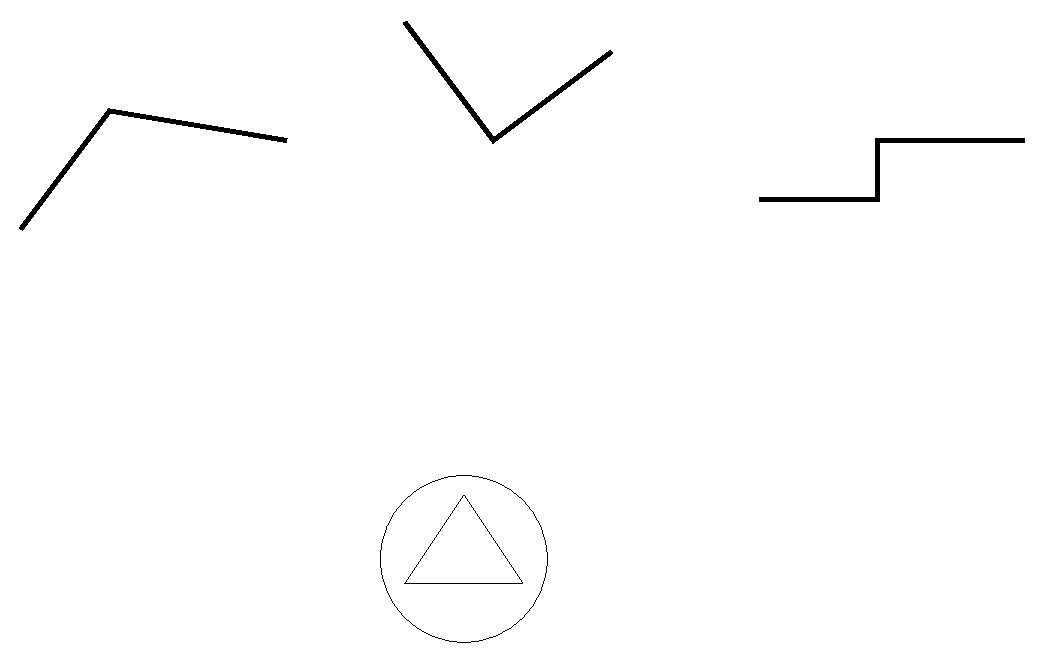
\includegraphics[width=5cm]{Pics/fig_corner_types}
  \caption{Corner types, from the left to the right: concave, convex,
  jump}
  \label{fig:corner_types}
\end{figure}

The corner detector algorithm distinguishes between three possible
types of corners: convex, concave and ``jump''. A ``jump'' corner is
defined as two parallel lines spaced a small distance apart. For
example doors in a hallway are classified by the algorithm as jumps.
It is possible to detect a convex corner even when only one side of it
is visible. We refer to such an observation as ``convex hidden''
corner. \refFigure{fig:corner_types} shows the different types of
corners.


\subsubsection{Algorithm}

The corner detector algorithm consists of two stages. During the first
stage the algorithm looks for regions in the laser scan that might
correspond to corners. During the second stage each corner hypotheses
is analysed more closely. Hypotheses that do not pass the tests are
discarded, those that remain are classified to be either convex,
concave, jump or convex hidden corners.

\begin{figure}[htbp]
  \centering
  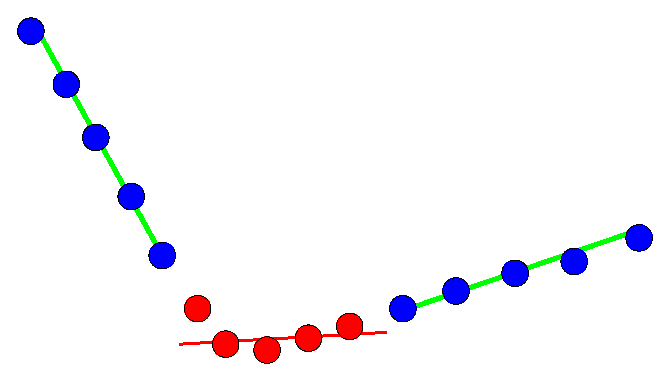
\includegraphics[width=5cm]{Pics/fig_corner_example}
  \caption{Trying to fit a line around the corner.}
  \label{fig:corner_example}
\end{figure}

During the first stage the algorithm looks at a narrow portion of the
laser scan (7 readings wide, that is only 3 degrees) and computes the
probability that this portion of the scan has been reflected from a
planar surface. To do that we fit a line to the laser scan points
and compute the average error squared from points to the fitted line.
High error implies low likelihood of the planar surface within the
region. We start with the right most region of the laser scan and move
it counter-clockwise with one laser reading increment.

As the window slides along the planar region of the scan the error
remains low. However when the region includes corners and other
irregularities, the error increases significantly, and hence the line
quality drops, refer to \refFigure{fig:corner_example}. Regions where
the line quality falls from high to low are suspects for possible
corners, see \refFigure{fig:corner_scan_example_b}.

Some laser rays fail to reflect back to the sensor, either because
there is no obstacle in the sensor range, or due to the reflective
properties of the surface. If there are any ``no return'' rays within
the window, the quality of the line for this window is set to the
lowest. One can see in \refFigure{fig:corner_scan_example_c}, the
effect it has. While most hypothesis actually correspond to true
corners in the environment, there is also a false hypothesis arising
from the sensor range limitations. However the second stage of the
algorithm successfully removes the false hypothesis.
\refFigure{fig:corner_scan_example_d} demonstrates this point.

\begin{figure}[htbp]
  \centering
  
  \subfigure[Scan is taken from right to left,
  counterclockwise. ]
 {
    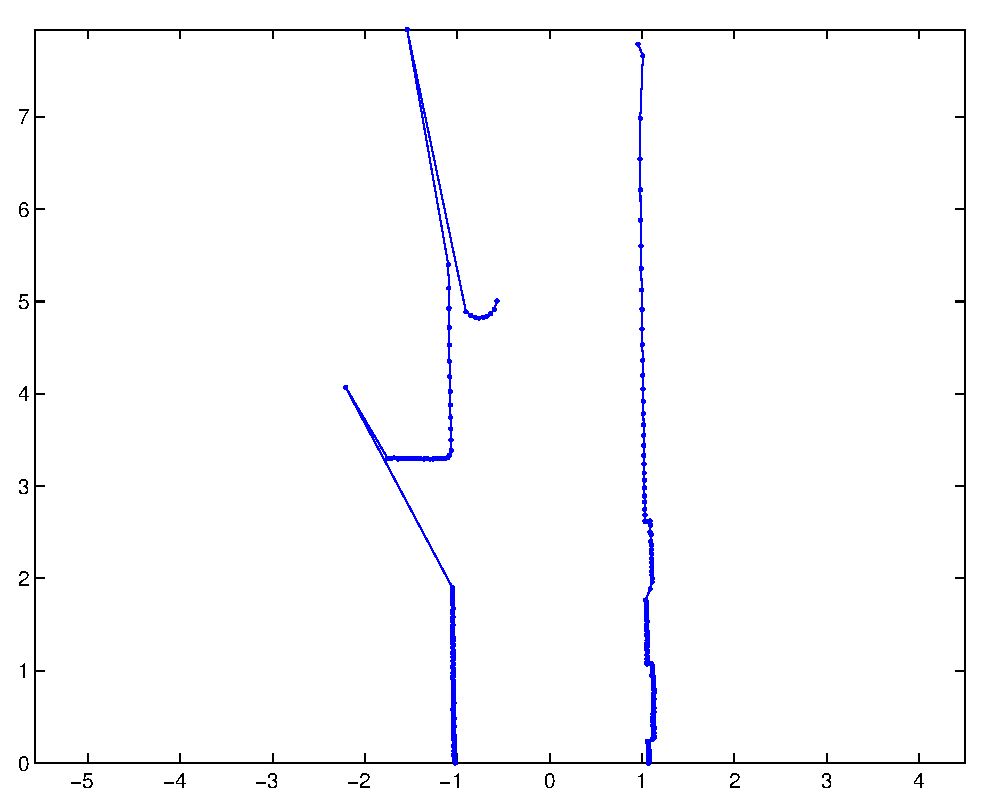
\includegraphics[width=6cm]{Pics/corner_scan_example_a}
  \label{fig:corner_scan_example_a}
} 
\subfigure[Negated total error squared is used as a measure of the
line quality. Horizontal line indicates good line threshold. Red lines
mark suspected corners.]{
  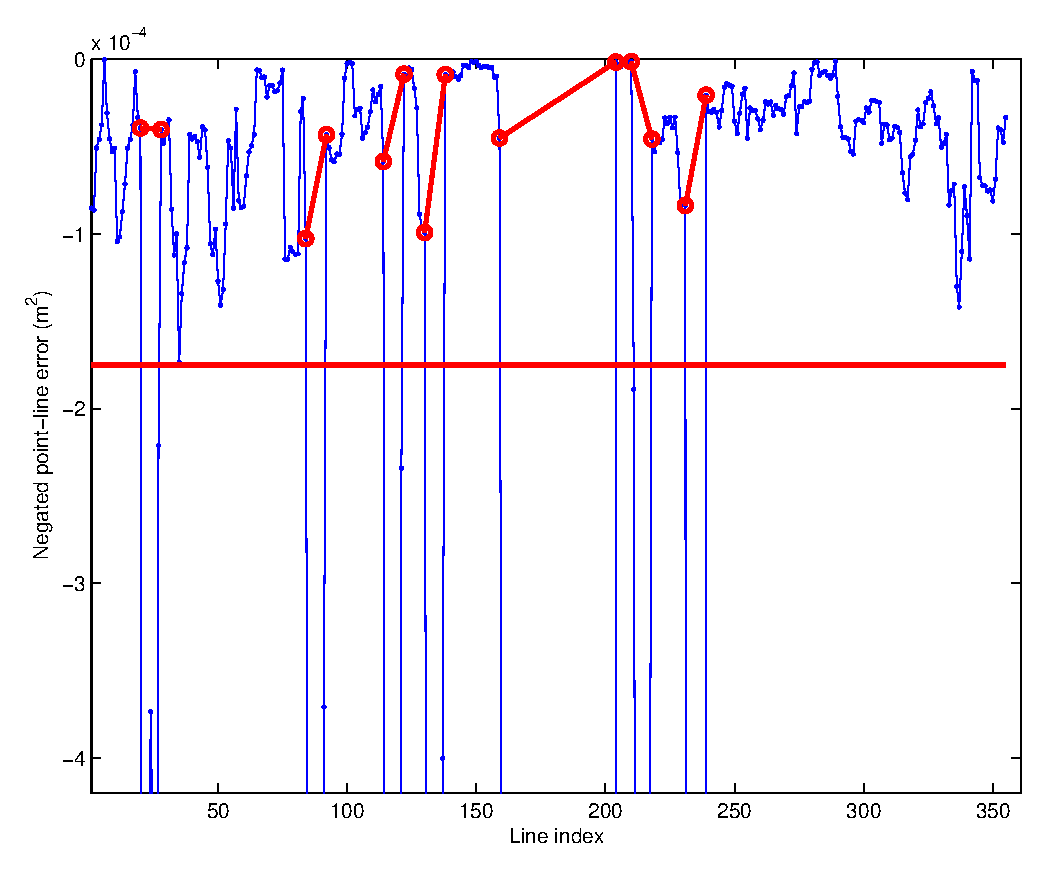
\includegraphics[width=6cm]{Pics/corner_scan_example_b}
  \label{fig:corner_scan_example_b}
}\\
\subfigure[Falls in line quality are suspect for corners. Circle
marks the beginning of the suspect region, square marks the end.]{
  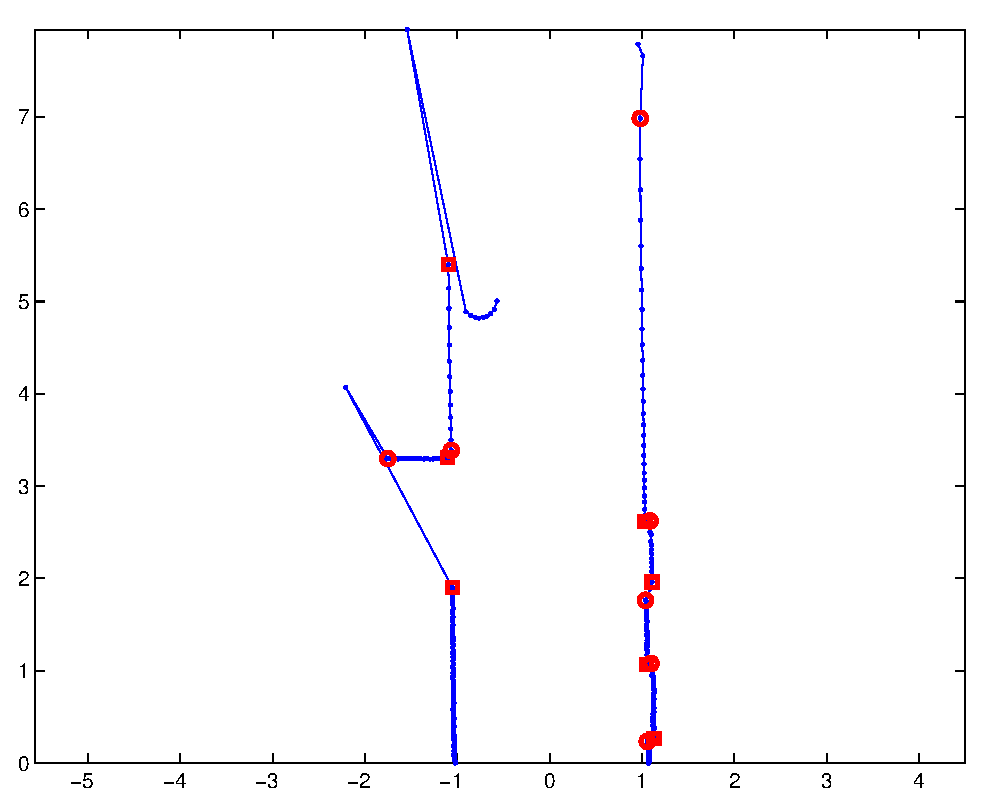
\includegraphics[width=6cm]{Pics/corner_scan_example_c}
  \label{fig:corner_scan_example_c}
}
\subfigure[Further tests confirm good corners and discard bad
ones. Corners are classified into several types.]{
  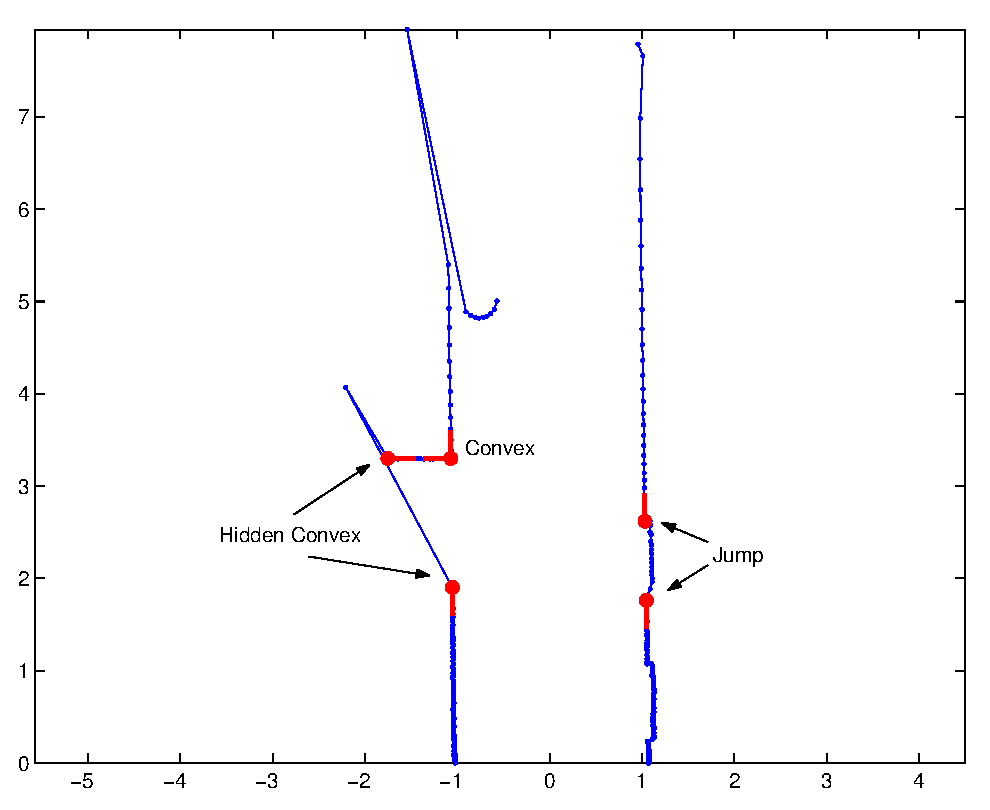
\includegraphics[width=6cm]{Pics/corner_scan_example_d}
  \label{fig:corner_scan_example_d}
}

\caption{Corner extraction from the laser scan.}
\end{figure}

The second stage of the corner detection algorithm classifies potential
corner observations as one of the: convex, concave, jump or convex
hidden corner, and discards those that do not fit either of the
models. Two intersecting lines to the left and to the right of the
suspected corner correspond to either convex or concave corner. Two
closely spaced collinear lines to the left and right of the corner
correspond to the ``jump'' corner. One line intersected by the laser
ray corresponds to the ``convex hidden'' corner.


\subsubsection{Uncertainty Representation}

A corner is considered to be a point landmark with extra attributes.
The extra attributes include the type of the corner and the
orientations of the corner arms. Overall there are four metric
parameters that define the corner: two parameters for the location and
two for the orientation of the corner arms. While it is possible to
compute the uncertainty directly from the laser readings, it is not
very obvious how to model error propagation. In this work we make some
simplifying assumptions to deal with this problem.  Errors in the
estimation of the corner position and the orientation of the corner
arms are assumed to be independent.

Observation of the corner location is expressed in polar coordinates.
Range and bearing measurements are assumed to be independent. Range
uncertainty is set to 5 per cent of the measured distance to the
corner plus some constant term.  Bearing uncertainty is set to 2
degrees. Uncertainty of the orientation of each arm is set to 3
degrees. While this is a very simplistic model of the uncertainty, in
practice it performs surprisingly well.


\subsection{Tree Trunk Detector}

Locations of tree trunks were extracted from the laser data using the
matlab code available from the ACFR website \cite{VP_dataset}.


\section{Mapping}

This section describes the implementation of the FastSLAM. It defines
the landmark update equations. Odometry models of vehicles used in the
experiment are also described.


\subsection{Point Landmarks}

Both trees and corners are treated as point landmarks. The extra
parameters, trunk diameter in the case of the tree landmark, and
orientation of the arms in the case of the corner landmark, are
assumed to be independent of the landmark position, and hence can be
estimated separately. The extra parameters are used for the data
association and for the computation of the probability of an
observation, given a landmark.

The point landmark is defined by its pose in the local reference
frame.

$$
{\bf x} = \left[ \begin{array}{c} x\\y \end{array} \right]
$$

The true state of the landmark is not known, the estimate of the landmark
state is maintained instead. The estimate of the landmark state at
time $k$ is $\hat{\bf x}_k$. The error covariance for the landmark
state is also maintained and is denoted $P_k$.

The landmark state is related to the observation by the following equation
$$
  {\bf z} = h({\bf x},v) = \left[
\begin{array}{c}
\sqrt{(x-x_s)^2 + (y-y_s)^2}\\ \noalign{\medskip}
\tan^{-1} \frac{y-y_s}{x-x_s} + \theta_s
\end{array}
\right] + v
$$
here $x_s$, $y_s$ and $\theta_s$ denote the location and heading of
the sensor in the local reference frame and $v$ is the observation noise,
assumed to be zero mean Gaussian.

The Jacobian of partial derivatives of $h$ with respect to landmark
state is

$$
H_{[i,j]} = \frac{\partial h_{[i]}}{\partial {\bf x}_{[j]}}
             \left(\hat{\bf x}_k , 0 \right).
$$

For clarity lets define the estimate of the landmark location in the
sensor centred coordinate frame as $\hat{x}' = \hat{x} - x_s$ and
$\hat{y}' = \hat{y} - y_s$. The Jacobian above is then equal

$$
H = 
 \left[ \begin {array}{cc}
   \frac{\hat{x}'}{ \sqrt{\hat{x}'^2+\hat{y}'^2} } & 
   \frac{\hat{y}'}{ \sqrt{\hat{x}'^2+\hat{y}'^2} } \\ \noalign{\medskip}
   \frac{-\hat{y}'}{ \hat{x}'^2+\hat{y}'^2 } & 
   \frac{ \hat{x}'}{ \hat{x}'^2+\hat{y}'^2 }.
\end{array} \right] 
$$

The Jacobian of partial derivatives of $h$ with respect
to noise is also needed by EKF, in this case it is trivial

$$
V_{[i,j]} = \frac{\partial h_{[i]}}{\partial v_{[j]}}
             \left(\hat{\bf x}_k , 0 \right) = I.
$$

These Jacobians are used to update the state of the landmark when a
new observation becomes available.


\subsubsection{Observation Update}

Every time the landmark is observed, its pose estimate is updated to
take into account the new information. This update is performed using
the standard Extended Kalman filter equations.


\subsubsection{Genesis}

When an observation does not match any of the existing landmarks, a
new landmark is added to the map. A range and bearing observation is
converted into a Cartesian coordinate space. The covariance of the
landmark is computed from the covariance of the measurement using
first order Taylor series approximation.


\subsection{XR4000: Odometry Model}

The robotic platform used for the indoor experiment is an XR4000 robot
from Nomadic Technology. This robot has a holonomic drive system with
four wheels. Controllers on-board the robot integrate distance
travelled by each of the wheels to compute the location of the robot
in some global reference frame. This estimate is subject to drift
due to the accumulation of errors in the process of integration. It is
difficult to model such a system from the physical principles, instead
we devise a simplified model.

The state of the robot at time $k$ is it's position and orientation in a
reference frame

$$
\x{k}{}{} = \left[\begin{array}{c} 
    x_k \\ 
    y_k \\ 
    \theta_k
  \end{array}\right].
$$

Being a holonomic robot, the XR4000 can move in any direction and rotate
at the same time, just like an office chair. We define control input
\U{k} to be an instantaneous translational and rotational velocity of
the robot at time $k$. Translational velocity is expressed in polar
coordinates $[v_k,\psi_k]^T$ in the robot centred frame. $\omega_k$ is
a rate of rotation of the robot centred frame relative to the
reference frame

$$
\U{k} = \Vector{v_k\\ \psi_k \\ \omega_k}.
$$

In the case of the XR4000, the state evolves according to the following
rule

$$
\x{k}{}{} = f(\x{k-1}{}{} ,\U{k-1}) = \x{k-1}{}{} + \Delta {\bf t}
\Vector{v_k\cos(\theta_{k-1} + \psi_{k-1})\\
v_k\sin(\theta_{k-1} + \psi_{k-1})\\
\omega_{k-1}}.
$$

Since \U{k} is not available directly it has to be derived from the
integrated robot poses returned from the on-board wheel controllers.
\U{k} is computed by the differentiation of the controller readings.

\begin{figure}[htbp]
  \centering

  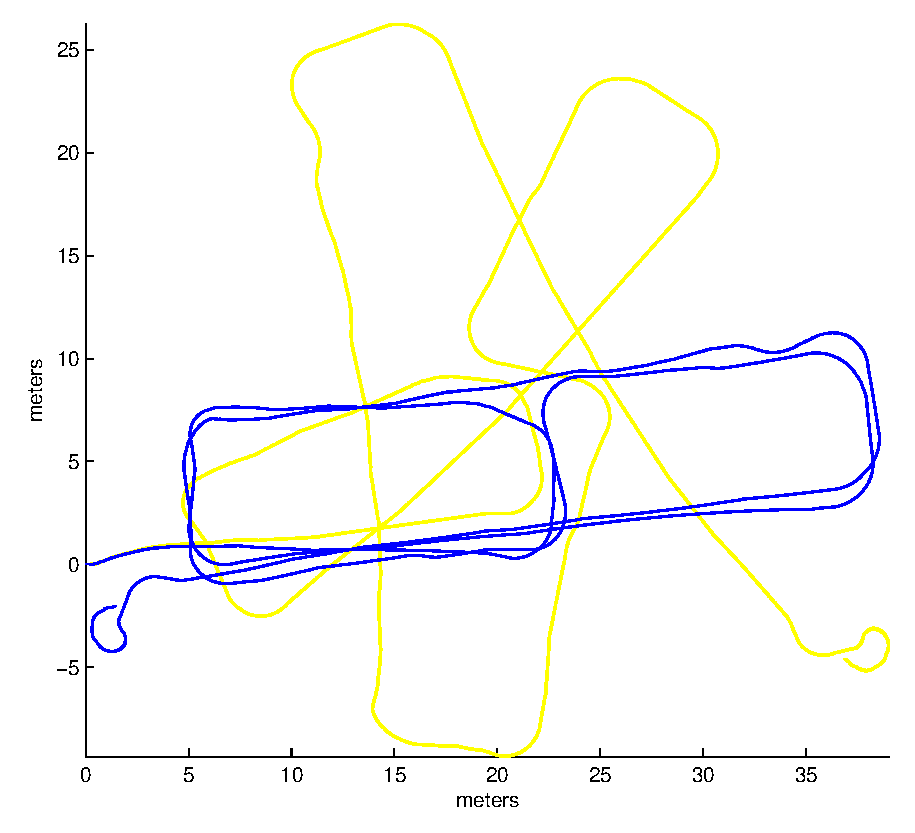
\includegraphics[width=10cm]{Pics/xr4000_raw_odo}
  
  \caption{XR4000 Odometry, before correcting for bias (light line)
    and after (dark line)}
  \label{fig:xr4000_raw_odo}
\end{figure}

{\bf Bias Correction}\\ The XR4000 used in this experiment has a
significant drift to the right, when travelling on a straight
line. Experiments revealed that, when the robot is instructed to
travel on a straight line forward, it actually follows an arc of 
100 meter radius, that corresponds to a rotation of $0.57^\circ$ to
the right per meter travelled. We correct for it by adjusting
rotational velocity $\omega_k$, and the heading of the translational
velocity $\psi_k$ accordingly.

When the robot is travelling on a curve, the bias is likely to be
different, however no experiments were conducted to estimate it. It is
assumed to be equal to that of the straight line.


\subsection{Truck: Odometry Model}

An Ackerman model is used to model the odometry of the truck used to
collect the Victoria Park data set. Sensor input: velocity of the left
rear wheel and angle of the front wheel. Velocity of the centre of the
vehicle $v_c$ is computed from the velocity of the left wheel $v_e$
using the following

$$
v_c = \frac{v_e}{1 - \tan \alpha \frac{H}{L}}.
$$

the state of the truck is defined by

$$
\Vector{x_k\\y_k\\\theta_k} = f(\x{k}{}{},\U{k}) = 
\x{k}{}{} + v_c \Vector{\cos \theta_{k-1} \\ \sin
  \theta_{k-1} \\ \frac{\tan \alpha}{L}} \Delta T.
$$


L=2.83m - distance between front and rear axles, H=0.76m - half the
distance between the rear wheels, sensor pose is 3.78m, 0.5m.

\subsection{Region Model: Indoors}

For the indoor experiment region extent was computed directly from the
laser scans. The first five scans are used to compute the free space in
front of the robot. This region defines the extent of the local map.
The occupancy grid is computed by a standard ray tracing algorithm.

\subsection{Region Model: Victoria Park}

In the outdoor environments free space dominates. It is therefore
possible to assign any region to the local map. So this is the
approach used in this case.

A grid map with the resolution of 50cm is used. Initial map region is
a rectangle aligned with robot heading direction. At the end of the
mapping the region is trimmed, refer to
\refFigure{fig:initial_region_vision}, it is set to the intersection
of the initial region and the region formed by the convex hull of the
map.

\begin{figure}[htbp]
  \centering
  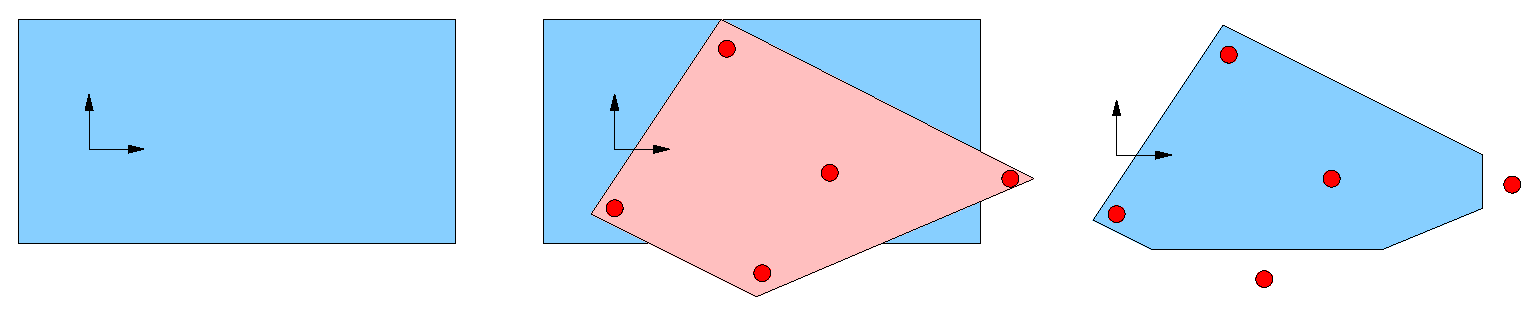
\includegraphics[width=14cm]{Pics/fig_convex_reg}
  \caption{Example of region evolution: start with a polygon regions,
  after mapping is complete fit convex hull to the map, set region to
  the overlap between the initial region and the convex hull.}
  \label{fig:initial_region_vision}
\end{figure}

\section{Experiment Setup and Analysis}

Particle filters produce different output for the same input (it is
the nature of the filter). As a result the performance of a particle
filter can not be judged based on just one execution of the
algorithm. 


%What quality measured can be used to judge the performance of a PF?
Traditionally a RMS (Root Mean Squared) distance from the estimate to
the true state is used to judge the quality of the PF. To use this
metric one needs to know the true state of the system. In the case of
a SLAM problem the path of the robot needs to be known. RMS is not a
very useful metric for the purposes of this thesis, since HTSLAM does
not produce a global estimate of the path. Even for global mapping
approaches this metric is of little use, since the RMS error is likely
to increase as the robot travels further away from the starting point.
High RMS error on the fringes of the map does not always suggest a bad
map, while even relatively low RMS error near the origin of the map
can indicate an inconsistent map.

Self-consistency is a more important measure of the quality of the
map, though it is harder to define and measure. In the ideal world the
definition can be simple: the map should contain all and only those
landmarks that exist in the environment and have been observed during
the experiment, all observations should be assigned to the correct
landmark. In real life experiments this condition will never hold.
Sensors do produce erroneous readings. Data association is often
ambiguous, especially in the environments where landmark density is
higher than the sensor uncertainty. Furthermore finding the true
correspondences between all landmarks and all observations is a
prohibitively laborious task.

\begin{figure}[htbp]
  \centering
  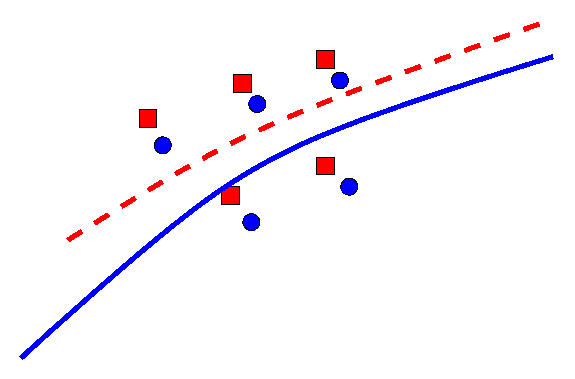
\includegraphics[width=5cm]{Pics/fig_inconsistent_map}
  \caption{Example of an inconsistent map. On a second pass through
    the region (dashed line), the robot failed data association and
    erroneously added new landmarks (squares).}
  \label{fig:inconsistent_map}
\end{figure}


The map self-consistency requirement needs to be relaxed to accommodate
for a realistic situation. In this work the following definition is
used: if the filter experiences systematic data association errors,
and divergence from the ground truth path, then the map is considered
to be inconsistent. \refFigure{fig:inconsistent_map} shows an example
of an inconsistent map. Errors like these are easy to spot for a human
operator with a priori knowledge of the environment.

The HTSLAM map is considered to be consistent if all local maps are
consistent, and if all relative map transformations are consistent.
Inconsistencies in relative local map poses can arise during loop
closing, when incorrect map correspondences are established.
Generally, inconsistent relative poses lead to inconsistent local
maps, and are therefor easy to detect. Failure to close the loop does
not result in the inconsistent map, however such a map provides less
information about the environment, and is therefor inferior to a
proper map.

\section {Results Indoors}

%Describe the environment.
Indoor experiments were performed on the third floor of the RSISE
building in ANU. A schematic of the environment is shown in
\refFigure{fig:rsise_level3_map}.

The HTSLAM algorithm will run 100 times on each data set. The map from
each run will be classified as one of: consistent and proper (closed
loop), consistent but improper (failed to close the loop) or
inconsistent.

 
\begin{figure}[htbp]
  \centering
  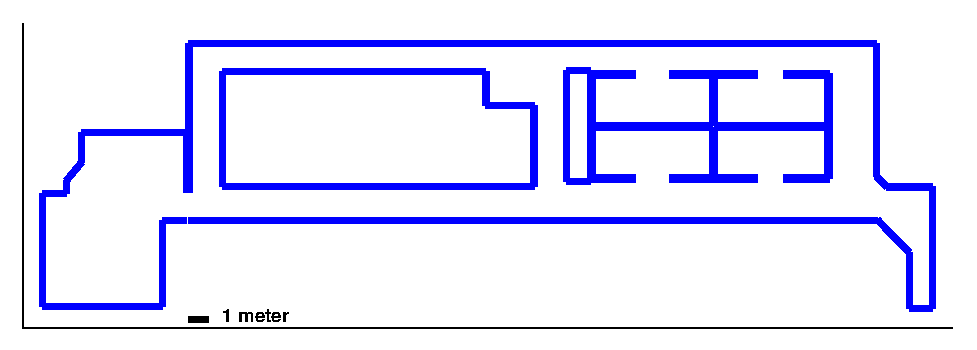
\includegraphics[width=13cm]{Pics/rsise_level3_map}
  \caption{RSISE level 3.}
  \label{fig:rsise_level3_map}
\end{figure}

The same data set was processed with 100 and 300 particles. One
hundred runs, each with a different random seed, were taken to discard
the possibility of a ``lucky run''. All of the runs have produced
correct maps on this particular data set.

\refFigure{fig:corner_map_100p} shows one of the maps built with
one hundred particles. Local maps are projected into the reference frame
of the first map. Note that no post-processing was done to align the
maps. \refFigure{fig:corner_map_300p} shows one of the maps produced
with 300 particles. The paths of all runs projected into the reference
frame of the first map are presented in
\refFigure{fig:corner_odo_all}. As expected, there is more variance
further from the origin.


\begin{figure}[htbp]
  \centering
  \subfigure[Projection of the HTSLAM map in the reference frame of map 1.]{
    \includegraphics[width=15cm]{Pics/corner_map_100p}
  }
  \subfigure[Topological path of the robot.]{
    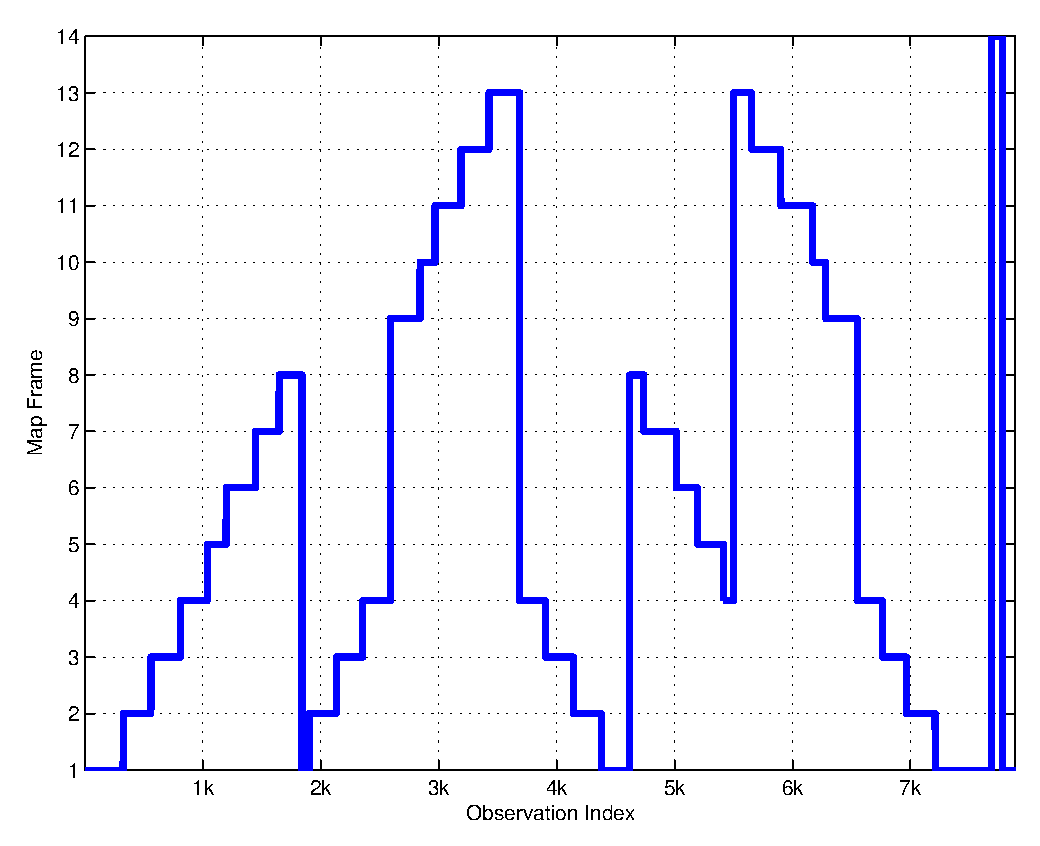
\includegraphics[width=10cm]{Pics/corner_odo_100p}
  }
  \caption{Map of corners (100 particles)}
  \label{fig:corner_map_100p}
\end{figure}

\begin{figure}[htbp]
  \centering
  \subfigure[Projection of the HTSLAM map in the reference frame of map 1.]{
    \includegraphics[width=15cm]{Pics/corner_map_300p}
  }
  \subfigure[Topological path of the robot.]{
    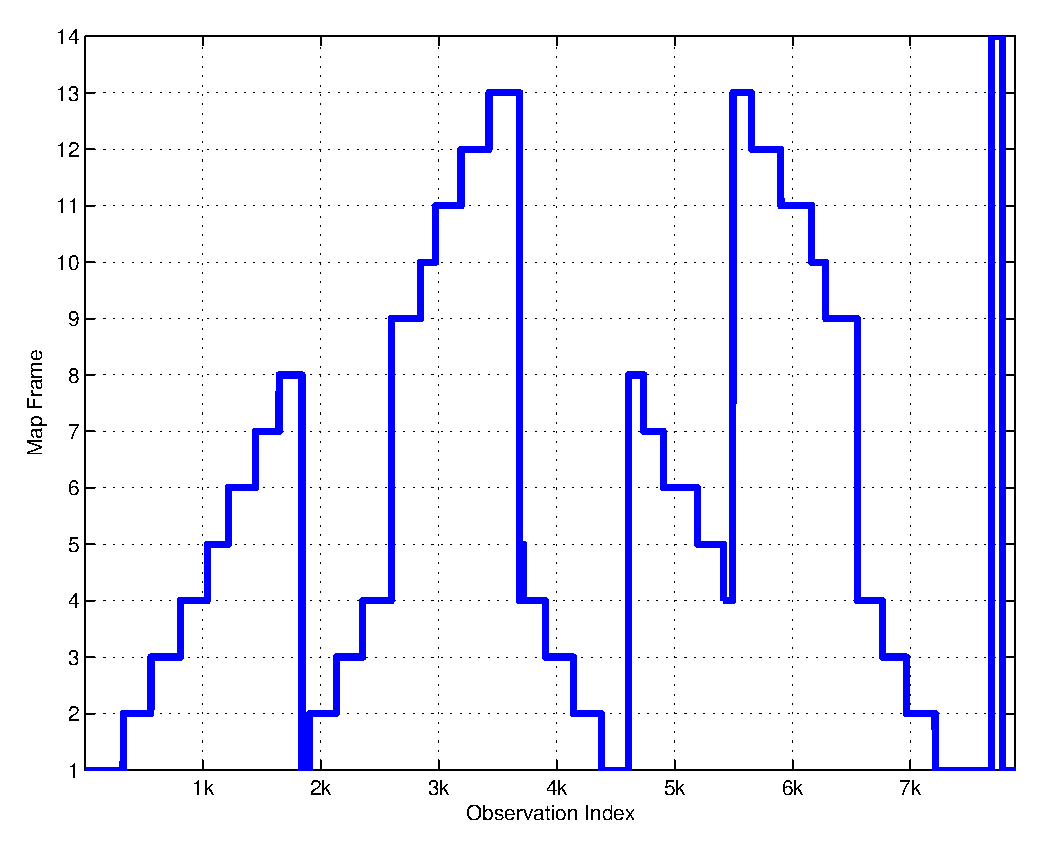
\includegraphics[width=10cm]{Pics/corner_odo_300p}
  }
  \caption{Map of corners (300 particles)}
  \label{fig:corner_map_300p}
\end{figure}

\begin{figure}[htbp]
  \centering
  \subfigure[100 particles]{
    \includegraphics[width=15cm]{Pics/corner_odo_all_100p}
  }
  \subfigure[300 particles]{
    \includegraphics[width=15cm]{Pics/corner_odo_all_300p}
  }
  \caption{Global Path over 100 test runs.}
  \label{fig:corner_odo_all}
\end{figure}


\subsection{Execution time}


\begin{figure}[htbp]
  \centering
  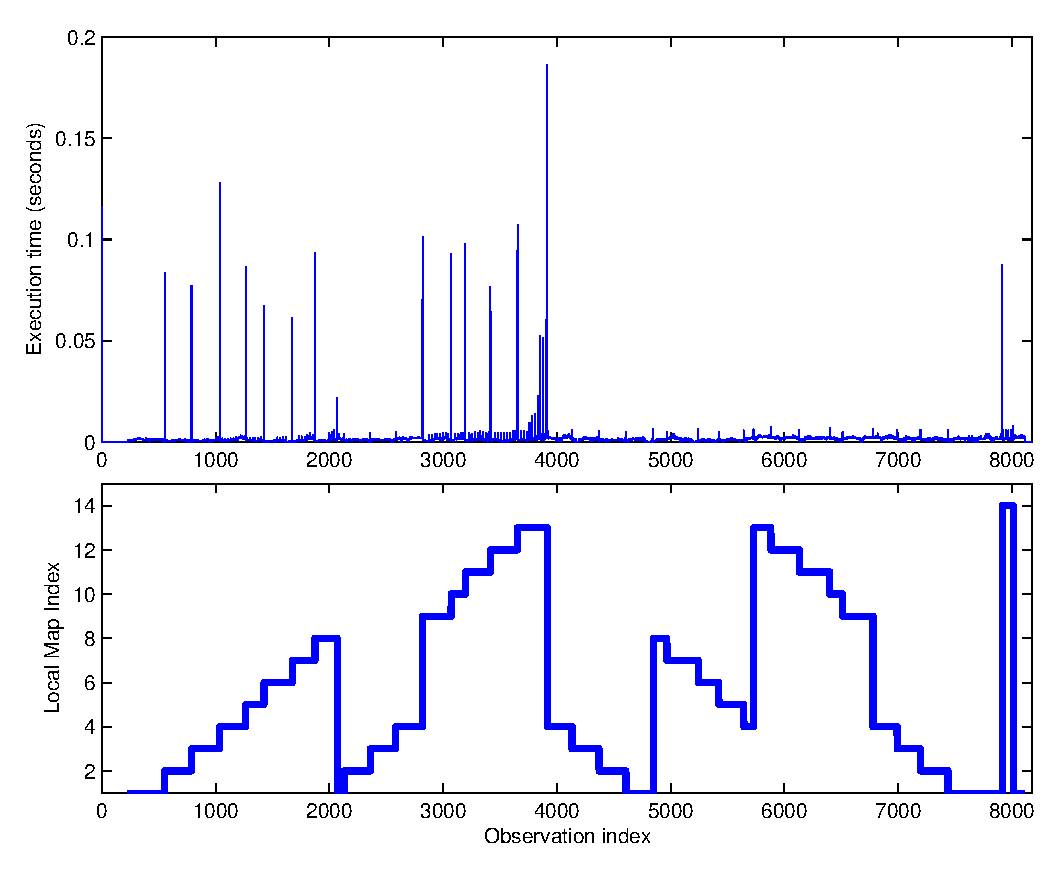
\includegraphics[width=15cm]{Pics/corners_execution_time}
  
  \caption{Execution time 100 particles.}
%map 33
  \label{fig:corners_execution_time}
\end{figure}

\refFigure{fig:corners_execution_time} shows the plot of execution
time per laser reading for one of the runs (100 particles were used).
The spikes in the execution time correspond to the creation of the new
region. Most of this time is spent computing the occupancy grid of the
region. Note that the graph never goes above 0.2 seconds, which is a
time between observations in case of the SICK laser range finder. The
algorithm runs faster than real-time. An important observation is that
computation time remains constant throughout the experiment.

\section {Results Victoria Park}

The Victoria park data set has been processed in a similar manner to
the indoor data set: 100 randomised runs of 100 and 300
particles. While the majority of the runs have produced a correct map,
some have failed. Table~\ref{tab:results_victoria_park} shows the
proportion of successful runs for 100 and 300 particles.

\begin{table}[ht]
\center
\begin{tabular}{r|c|c|c}
Num. Particles & Consistent & Consistent but improper & Inconsistent\\
\hline
100 & 75  & 0 & 25 \\
300 & 93  & 0 & 7\\
\end{tabular}
\caption{Summary of the experiments on the Victoria Park data set.}
\label{tab:results_victoria_park}
\end{table}

As one would expect, an increase in the number of particles produces a
more robust mapping. 

\refFigure{fig:trees_map_100p} and \refFigure{fig:trees_map_300p} show
an example of a correct map for 100 and 300 particles
respectively. \refFigure{fig:trees_odo_all} shows paths of all runs
projected in to the reference frame of the first map.


\begin{figure}[htbp]
  \centering
  \subfigure[Projection of the HTSLAM map in the reference frame of map 1.]{
    \includegraphics[width=15cm]{Pics/trees_map_100p}
  }
  \subfigure[Topological path of the robot.]{
    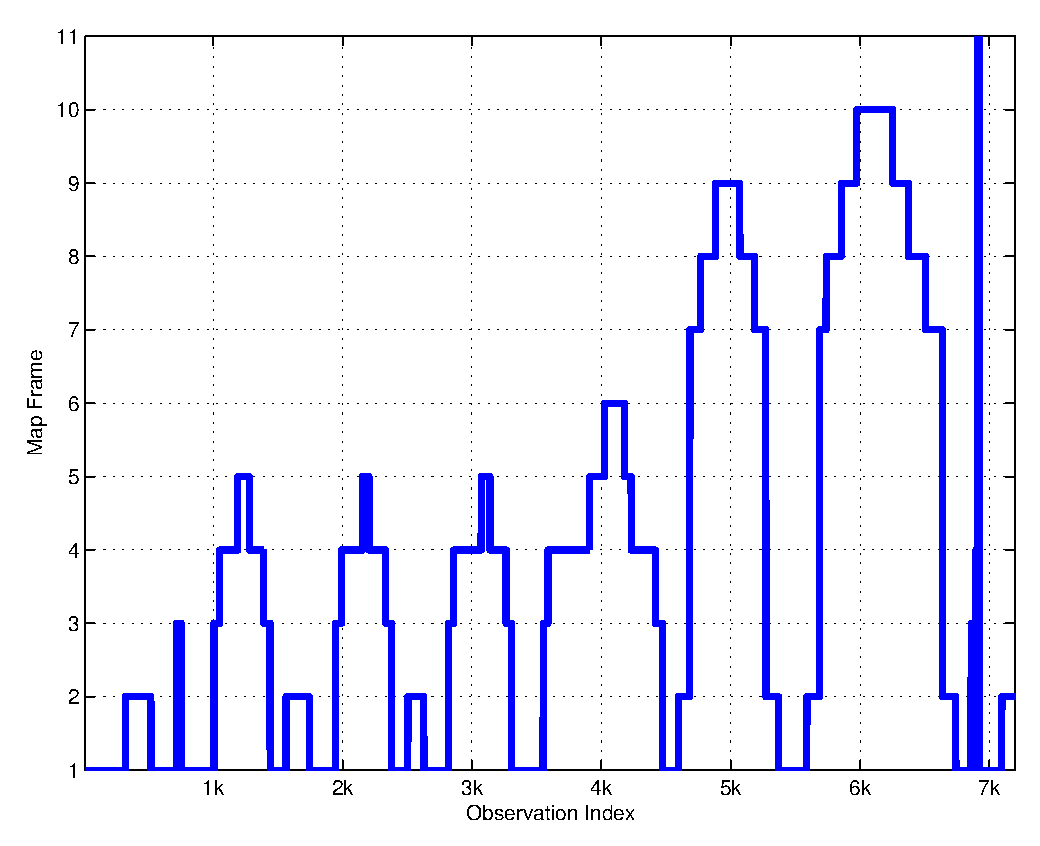
\includegraphics[width=10cm]{Pics/trees_odo_100p}
  }


  \caption{Map of corners (100 particles)} %map 33
  \label{fig:trees_map_100p}
\end{figure}

\begin{figure}[htbp]
  \centering
  \subfigure[Projection of the HTSLAM map in the reference frame of map 1.]{
    \includegraphics[width=15cm]{Pics/trees_map_300p}
  }
  \subfigure[Topological path of the robot.]{
    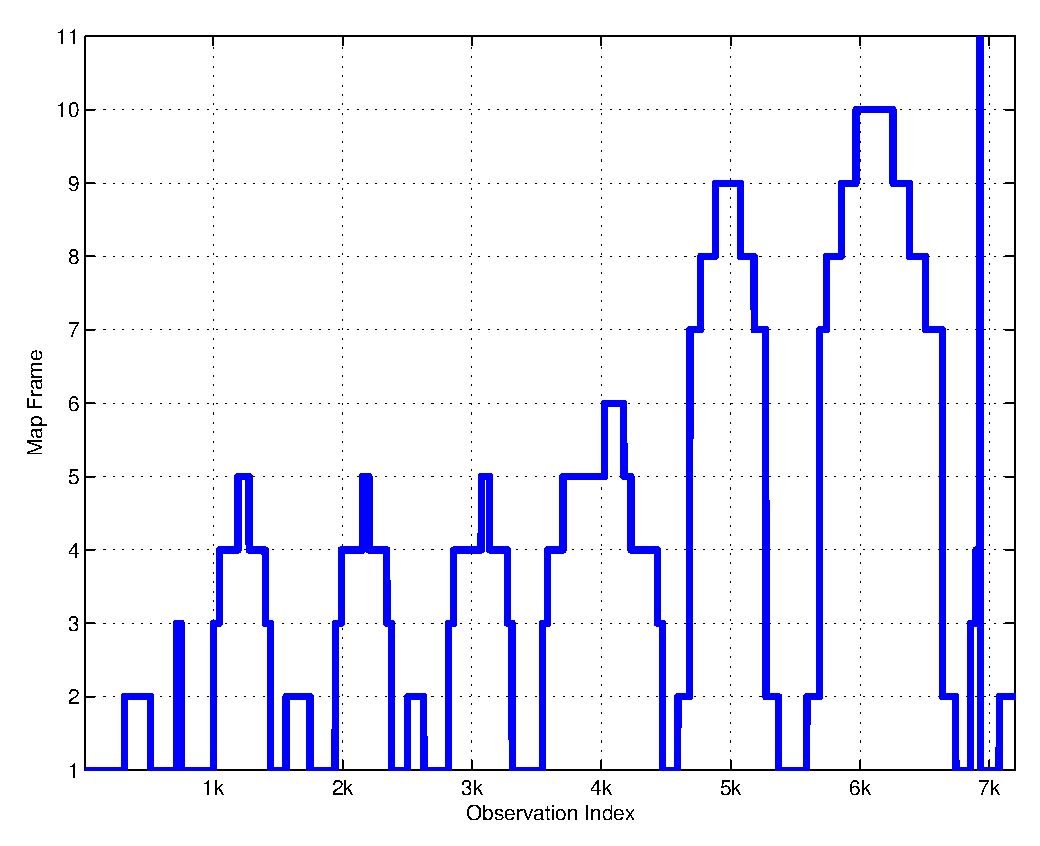
\includegraphics[width=10cm]{Pics/trees_odo_300p}
  }


  \caption{Map of corners (300 particles)} %map 33
  \label{fig:trees_map_300p}
\end{figure}

\begin{figure}[htbp]
  \centering
  \subfigure[100 particles]{
    \includegraphics[width=10cm]{Pics/trees_odo_all_100p}
  }
  \subfigure[300 particles]{
    \includegraphics[width=10cm]{Pics/trees_odo_all_300p}
  }
  \caption{Global Path over 100 test runs.}
  \label{fig:trees_odo_all}
\end{figure}







% LocalWords:  Odometry HTSLAM Pics odo EKF XR holonomic matlab ACFR FastSLAM
% LocalWords:  Kalman RSISE ANU


\chapter{Experimental Results: Vision}
\label{chpt:Vision_Results}
\section{Sensor Description}

The sensor used in the experiment consists of a stereo pair of
cameras. The cameras are mounted on an XR4000 robot facing forward,
parallel to the ground plane. The two cameras are aligned parallel to
one another. The stereo baseline is approximately 30 cm. The relative
pose of the cameras were computed by stereo calibration
\cite{zhang1999fcc}. Internal camera parameters were determined by
calibration for each of the cameras \cite{zhang1999fcc}. 

The cameras are capable of capturing colour images at a maximum
resolution of 640x480 at the rate of 30 frames per second with
interlacing, however the recoding system on-board of the robot can
sustain a much lower throughput. The capturing system records only odd
fields (320x480) at an average rate of 11.5 frames per second per
camera.

\begin{figure}[htbp]
  \centering
\subfigure[Original image.]{
  \includegraphics[width=12cm]{Pics/barrel_distortion}
}\\
\subfigure[Corrected image.]{
  \includegraphics[width=12cm]{Pics/undist_barrel_distortion}
}

  \caption[Barrel distortion]{Effect of barrel distortion.}
  \label{fig:barrel_distortion}
\end{figure}

The cameras used in this experiment have a noticeable barrel
distortion that is corrected in software. The correction is applied
off-line. \refFigure{fig:barrel_distortion} shows an example of
original and corrected images.


\section{Feature Detector: Vertical Edges}

Vertical edges are common in human built environments, and can be
detected fast and reliably. A matched pair of edges in two images
corresponds to a line in world coordinates. A matched pair of vertical
edges corresponds to a vertical line in the world if both
cameras are parallel to the ground plane. A vertical line in a three
dimensional space has only two degrees of freedom and can be defined
completely by a point of intersection with the ground plane. Similarly,
a vertical line in an image plane can be defined completely by a
single parameter: its distance from the left side of an image. A
camera detecting vertical edges is effectively a planar bearing-only
sensor.

By reducing the dimensionality of the sensor from 3d to 2d the
observation model is simplified, which in turn simplifies uncertainty
modelling. Since the robot motion is restricted to the plane, the
vertical dimension can be safely ignored.

The most problematic part of the bearing only SLAM is landmark
creation. One needs at least two bearing observations from different
poses to compute an estimate of landmark location. There are a
number of techniques commonly used \cite{bearing_only_slam}. Since the
robot in this experiment has two cameras, the problem of creating a
new landmark is simplified significantly. Having two cameras also
assists in the data association process. 

The first step of the algorithm is the detection of vertical edges in
the left and right images using vertical Sobel edge detector
\cite{Hartley2004}. To make feature detection more robust, short edges
are discarded as these are more likely to be spurious. Edges that are
only few pixels apart are also removed at this stage.

In the second step correspondences between edges in the left and right
images are established. The cameras on the robot are aligned to be
parallel, and as a result epipolar lines are along the $x$
axis\cite{Hartley2004}. Normalised cross-correlation is used to
establish initial matches. Matches with correlation higher than a
predefined threshold are accepted. If too many matches ($>5$) are
found for a particular edge, this edge is removed. Edges that had no
correspondence are also removed. For the remaining edges the best
three matches are considered.

It is clearly impossible that two distinct edges in the left image
appear in the same spot in the right image, without one being hidden
by another, in which case the depth of the edges cannot be
determined. The matching process has to consider all pairwise matches
to avoid matching the same edge in one image to several edges in the
other.

One can visualise this problem as a graph: every pair of matched edges
defines a node in the graph. Nodes of the graph that do not share a
common edge in both images are connected. The largest fully connected
sub-graph of this graph (commonly referred as ``clique'' or ``maximal
clique'' of a graph) corresponds to the largest set of compatible edge
matches. The problem of finding the clique of a graph is NP complete
\cite{cook1971ctp}, which is intractable for a large set of
features. There are, however, methods that can find an approximate
solution \cite{balas1986fmc,pardalos1994mcp}. The approach adopted in
this work is a simple greedy search algorithm with the following steps:

\begin{enumerate}
\item Sort matches in descending order according to their normalised
  cross-correlation results.
\item Set output set to empty.
\item Take one item from the top of the sorted input set.
\item If compatible with all elements in the output set, add it to the
  output set, else discard.
\item Repeat 3 and 4 until the input set is empty.
\end{enumerate}

The compatibility step in the algorithm above can be implemented to
have a constant time computational complexity. The overall
computational complexity of the algorithm is therefore $O(N \log N)$ -
the complexity of the sort.

\begin{figure}[htbp]
  \centering
  \includegraphics[width=13cm]{Pics/example_edge_detector}
  \caption[Edge Detection Example]{Edge Detection Example: the two
    video frames from the left and right cameras are shown in the
    upper row, the plot below shows location of the edges in the
    sensor centric reference frame and their corresponding
    uncertainties.}
  \label{fig:example_edge_detector}
\end{figure}

An example of vertical edge detection is shown in
\refFigure{fig:example_edge_detector}. Edge correspondences are
indicated by colour: a blue edge in the left corresponds to a blue
edge in the right image, green to green, and so forth. Locations of
the features in the reference frame of the left camera are also
shown. Landmark uncertainty is also shown. Note that Cartesian
uncertainty is only used for initialisation of landmarks. Landmark
update equations assume a bearing-only model.

The appearance of a feature provides important information to the
mapping module by assisting in data association. This is especially
useful in situations when two edges are very close spatially (like
the cyan and magenta edges (edges 4 and 5, counting from the left) in
the \refFigure{fig:example_edge_detector}).

Since vertical edges are generally uniform along the vertical
dimension, the edge template can be ``compressed'' by computing the
average intensity along the vertical dimension. The experiments
presented use a template width of 7 pixels. Since all three colours
per pixel are considered, each template is represented by 21 integer
values. Using only 7 pixels per feature (21 values) greatly reduces
computational effort for template matching. Templates are also
normalised to have zero mean, making correlation computation fast (21
multiplications and 20 additions in this case). Normalisation also
makes template matching less sensitive to variations in lightning
conditions.

\subsection{Sensor Uncertainty}

There are several sources of uncertainty in the sensor. Some
uncertainty comes from the fact that camera calibration is not
perfect. The camera focal length $F$ and principal point $C$ are not
known exactly and might also vary slightly during the experiment. A
second source of uncertainty is the feature extraction mechanism. As
point of view changes, an edge might be detected on a slightly
different part of a physical object. Furthermore, discretisation
errors might add noise as well.

Bearing observation is computed from the column pixel $p$ using the
following equation

$$
z = f([p,C,F]^T) = \frac{p - C}{F}.
$$

The Jacobian of $f$ with respect to $[p,C,F]^T$ ,$\bigtriangledown f$, is used to compute the
approximate Gaussian uncertainty of $z$ from the uncertainties of
$[p,C,F]^T$:

$$
\bigtriangledown f = \left[ 
\frac{1}{F},
\frac{1}{-F},
\frac{-p + C}{F^2}
\right].
$$

The uncertainty of the bearing is then 

$$
\sigma^2_z = \bigtriangledown f \left[ \begin{array}{ccc}
      \sigma^2_p & & \\
   &  \sigma^2_C & \\
  & & \sigma^2_F 
\end{array} \right] \bigtriangledown f^T.
$$



\section{Edge Landmarks}

An edge landmark may be treated as a point landmark with some
additional attributes. The extra attributes include the normalised
edge template (7 pixel x 3 colours = 21 values) and a list of all
observations of the landmark.  The normalised average template is used
to aid in data association and also during the map matching when
closing loops. A list of observations is also used during data
association if the result of matching with the average template failed
to produce a definitive answer.

The data structure used to hold the list of observations can be copied
in constant time, so there is no undue computational burden for
keeping this information. Memory requirements however grow as more
observations are collected. It is not absolutely necessary to keep all
this information, as the average template is usually sufficient. The
main motivation for doing so is to allow accurate template matching in
situations where the appearance of the landmark changes significantly
with observation angle.

The goal of keeping templates is to provide a comprehensive
representation of the appearance of the landmark from various view
points. This can be achieved with relatively few templates. It is not
necessary to store all of them. An approach like principal component
analysis \cite{jolliffe2002pca} can be used to find a sufficient set
of templates for a given edge feature. This problem is, however, beyond
the scope of this thesis.

The true landmark state ${\bf x} = \left[x,y \right]^T$ represents its
location in the local reference frame. The camera pose in the local frame
is denoted $x_c,y_c$ and camera orientation is $\theta_c$. For clarity,
define $x'=x-x_c$ and $y'=y-y_c$. Observation $z_k$ and
landmark states are related by the non-linear function $h$, defined by
($v = N(0,\sigma_{v}^2)$ is a measurement noise)

$$
z_k = h({\bf x},v) =
\frac{-x'\sin \theta_c + y' \cos \theta_c }
     {+x'\cos \theta_c + y' \sin \theta_c } + v.
$$

The true state of the landmark is not known, but the estimate of the
landmark state at time $k$, $\hat{\bf x}_k$, is available. The
estimated covariance of the landmark is maintained by the EKF
and is denoted $P_k$. For clarity, define also
$\hat{x_k}'=\hat{x_k}-x_c$ and $\hat{y_k}'=\hat{y_k}-y_c$.

Additionally, define a Jacobian of partial derivatives of $h$ with
respect to the landmark state:

$$
H_{[i,j]} = \frac{\partial h_{[i]}}{\partial {\bf x}_{[j]}}
             \left(\hat{\bf x}_k , 0 \right).
$$

It is equal to

$$
  H = \left[ 
\begin{array}{c}
\frac{-\hat{y_k}'}
{\hat{x_k}'^2 \cos^2 \theta_c + 2\hat{x_k}'\hat{y_k}'\cos\theta_c\sin\theta_c + \hat{y_k}'^2\sin^2  \theta_c }\\
{}\\
\frac{\hat{x_k}'}
{\hat{x_k}'^2 \cos^2 \theta_c + 2\hat{x_k}'\hat{y_k}'\cos\theta_c\sin\theta_c + \hat{y_k}'^2\sin^2 \theta_c }
\end{array}
      \right].
$$

These Jacobians are used by the EKF, and also during data association,
to project landmark uncertainty into the observation space.

The Jacobian of partial derivatives of $h$ with respect
to noise is also needed by the EKF, and in this case it is trivially

$$
V_{[i,j]} = \frac{\partial h_{[i]}}{\partial v_{[j]}}
             \left(\hat{\bf x}_k , 0 \right) = 1.
$$


\subsection{Data Association}

First, all landmarks are projected into the observation space, both
into the left and right camera. Those landmarks that fall outside the
sensor range are discarded. For each observation the most likely
landmark is found using the nearest neighbour search. 

The quality of a match between a landmark and a single bearing
observation is computed using the following:

$$
  {\bf w}_k = \int p(z_k|^z{\bf x}_k)p(^z{\bf x}_k) d^z{\bf x}.
$$

Here $^z{\bf x}_k$ is a landmark projected into the camera plane, and
$p(^z{\bf x_k})$ is approximated to be a Gaussian, EKF style:

$$
p(^z{\bf x}_k) = N(h(\hat{\bf x}_k,0), H P_k H^T).
$$

The term $p(z_k|^z{\bf x}_k)$ represents the measurement uncertainty
and is also a Gaussian distribution $N(z_k ,\sigma^2_{vk})$. Since
both distributions are Gaussians, the integral of their product can be
computed analytically.

Both left and right bearing have to match the landmark. The total
quality of the match is a product of the left and right weights ${\bf
  w}^l_k{\bf w}^r _k$.

Template matching is used to aid data association as a binary pass or
fail operator. Template matching is only performed if the spatial
tests have passed.

Nearest neighbour is the most common approach to data association, due
to its simplicity, however there are some drawbacks to this
method. The fact that observations were extracted from the same video
frame provides an important piece of information - that these
observations are of different physical entities. Nearest neighbour
search discards this information. Different observations from the same
video frame can be assigned to the same landmark.

Ideally the data association process should take all available
information into consideration. One can use the joint compatibility
data association \cite{neira01:_data_assoc_stoch_mappin_using}, or one
might explore the complete set of possible data associations directly
by sampling from the set of all possible data association decisions
\cite{nieto2003}. In this work nearest neighbour search assisted by
template matching proves sufficient, however a better data association
approach is likely to improve the success rate of the existing
approach.


\subsection{Observation Update}

An observation is treated as two independent bearing-only
observations, first left then right. The standard EKF update equations
are applied to update the estimate of the landmark state and its
covariance.

The landmark template is also updated. It is simply an average of all
observation templates. Each landmark maintains a count of the number
of times it has been observed and a sum of all templates. The average
template is computed from the sum by simply dividing by the total
number of observations. After that, the template is normalised such
that the mean is equal to zero and the sum of deviations from the
mean squared is equal to 1. The normalisation is pre-computed to speed up
the computation of normalised cross correlation.


\subsection{Genesis}

When an edge pair does not match any of the existing landmarks in
the map, a new landmark is added to the map. The initial landmark pose
and the corresponding uncertainties are computed from the observations
using the equations described below.

Let $x_r,y_r$ be the location of the right camera with respect to the
left one and $\theta_r$ be the orientation of the right camera
relative to the left one. Let $u_l,u_r$ be the bearing observations
(tangent of the angle) from the left and right cameras
respectively. Observation is defined to be

$$
{\bf z} =  \left[
    \begin{array}{c}
       u_l\\u_r\\x_r\\y_r\\\theta_r
    \end{array}
\right].
$$

The landmark state can be computed from the observation using the
following:

$$
{\bf x} = f\left({\bf z}\right) 
= \left[\begin{array}{c}
\frac{y_r - x_r\tan(\tan^{-1} u_r+\theta_r)}{u_l-\tan(\tan^{-1} u_r+\theta_r) }\\
{}\\
\frac{y_r - x_r\tan(\tan^{-1} u_r+\theta_r)}{u_l-\tan(\tan^{-1} u_r+\theta_r)}u_l
\end{array}
\right].
$$

Assume that the uncertainty of the observation is a Gaussian with
the following block-diagonal covariance matrix:

$$
C_z = \left[
  \begin{array}{ccc}
    \sigma^2_{ul} &             & \\
                & \sigma^2_{ur} & \\
                &             & \Sigma_{xy\theta}
  \end{array}
\right].
$$

Computing the Jacobian of $f$ with respect to each of the
observation elements,

$$
{\bf J}_{[i,j]} = \frac{\partial f_{[i]}}
{\partial z_{[j]}}\left(z \right)
$$

the initial uncertainty of the feature is then:

$$
P = {\bf J} C_z {\bf J}^T.
$$

The landmark template is initialised to that of the observation.

\section{Defining Map Region}

Unlike laser range sensors, vision sensors cannot provide free space
information easily. It is therefore assumed that no free space
information is available. The approach for defining region boundaries
is identical to that used for the Victoria park data set, with an
exception of the size of the initial region and the size of grid
cells, which were set to be smaller.

\section{Results}

Vision data has been collected together with the laser corner data so
that a comparison can be made between vision and laser
experiments. The vision data set was processed with 100 and 300
particles. One hundred runs of the algorithm were taken to judge the
robustness of the algorithm (100 for 100 particles and 100 for 300
particles).
%\subsection{Maps}

Figures~\ref{fig:edge_map_300p} and \ref{fig:edge_map_100p} show the
map produced for one of the runs using 300 and 100 particles
respectively. Local maps are projected into the reference frame of the
first region. 

Vision is a much more challenging sensor than laser. While most of the
runs have produced good map, many runs
failed. Table~\ref{tab:results_vision} lists the success/failure rates
for the experiment.

\begin{table}[ht]
\center
\begin{tabular}{r|c|c|c}
Num. Particles & Consistent & Consistent but improper & Inconsistent\\
\hline
100 & 67 & 1 & 32\\
300 & 71 & 5 & 24\\
\end{tabular}
\caption{Vision indoors: Summary of the experiments.}
\label{tab:results_vision}
\end{table}

Increasing the number of particles makes the algorithm more robust,
but only slightly. Figures~\ref{fig:edge_map_300p_broken} and
\ref{fig:edge_map_300p_borken2} show examples when HTSLAM did not
succeed to build a proper map. \refFigure{fig:edge_odo_all} shows the
paths of all 100 experiments projected into the reference frame of the
first region.

%Refer to the laser results, same data set. 

\begin{figure}[htbp]
  \centering

  \subfigure[Projection of the HTSLAM map in the reference frame of map 1.]{
    \includegraphics[width=15cm]{Pics/edge_map_300p}
  }\\
  \subfigure[Topological path of the robot.]{
    \includegraphics[width=10cm]{Pics/edge_odo_300p}
  }

  \caption{Vision indoors: Map of edges (300 particles/map 52)}
  \label{fig:edge_map_300p}
\end{figure}

\begin{figure}[htbp]
  \centering
  \subfigure[Projection of the HTSLAM map in the reference frame of map 1.]{
    \includegraphics[width=15cm]{Pics/edge_map_100p}
  }
  \subfigure[Topological path of the robot.]{
    \includegraphics[width=10cm]{Pics/edge_odo_100p}
  }
  \caption{Vision indoors: Map of edges (100 particles/map 89)}
  \label{fig:edge_map_100p}
\end{figure}

\begin{figure}[htbp]
  \centering
  \subfigure[Projection of the HTSLAM map in the reference frame of map 1.]{
    \includegraphics[width=15cm]{Pics/edge_map_300p_broken}
  }
  \subfigure[Topological path of the robot.]{
    \includegraphics[width=10cm]{Pics/edge_odo_300p_broken}
  }
  \caption{Vision indoors: Jumped out, failed to come back(300 particles/map 40).  Topologically correct, but not ``optimal''}
  \label{fig:edge_map_300p_broken}
\end{figure}

\begin{figure}[htbp]
  \centering
  \subfigure[Projection of the HTSLAM map in the reference frame of map 1.]{
    \includegraphics[width=15cm]{Pics/edge_map_300p_broken2}
  }
  \subfigure[Topological path of the robot.]{
    \includegraphics[width=10cm]{Pics/edge_odo_300p_broken2}
  }

  \caption{Vision indoors: Failed transition 7 to 2 (300 particles/map
    18).}
  \label{fig:edge_map_300p_borken2}
\end{figure}

\begin{figure}[htbp]
  \centering
  \subfigure[100 particles]{
    \includegraphics[width=15cm]{Pics/edge_odo_all_100p}
  }
  \subfigure[300 particles]{
    \includegraphics[width=15cm]{Pics/edge_odo_all_300p}
  }
  \caption{Vision indoors: Global Path over 100 test runs.}
  \label{fig:edge_odo_all}
\end{figure}



\subsection{Error Analysis}

There are a number of reasons for a poorer performance of the vision
SLAM when compared to a corner detector in the same environment:

\begin{itemize}
\item Data association is quite challenging with this type of
sensor. 
\item Poor calibration of the sensor.
\item Unmodelled sensor error correlations.
\item Sub-optimal local region assignment
\end{itemize}

Data association is especially difficult when revisiting the region
when travelling in an opposite direction. The appearance of landmarks
can vary significantly when viewed from a different
angle. Furthermore, a very different set of landmarks is visible when
traversing a region in opposite direction. This makes transitions back
into a mapped region from a different direction prone to data
association errors.

Camera provides a rather accurate bearing measurement. As a result the
performance of the sensor is sensitive to calibration errors. The more
accurate your sensor is, the more obvious the impact of biases in the
error model will be.

Another important factor to consider is the effect of unmodelled
correlations between errors in individual observations. All features
detected in the same video frame share common source of uncertainty:
camera calibration parameters. Yet errors are assumed independent for
practical reasons.

As mentioned previously vision and corner data sets were collected from
the same platform at the same time, yet one can see that local region
assignment is significantly different between the two data sets. In
corner based SLAM occupancy grid was used to define a local region. In
the case of vision based experiment no free space information was
available, hence regions were assigned to be of fixed size. Using
free-space information for local region assignment is advantageous as it
partitions the space in a more sensible way. Consequently, local map
transitions are less reliable for a vision data set. This suggests that
a better model for local region assignment might be necessary.




% LocalWords:  epipolar EKF Jacobians Gaussians IDE Sobel  cyan discretisation
% LocalWords:  HTSLAM odometric odometry Jacobian


\chapter{Conclusion}
This thesis has presented a novel approach to mapping that combines
metric and topological information to build maps of medium to large
environments. In HTSLAM metric and topological representations are
equally important. HTSLAM does not aim to build a global metric map
with a single reference frame. Instead, each local region has its own
reference frame. Relative poses of neighbouring regions are maintained
in the topological structure of a HTSLAM map. The proposed map
structure facilitates computation of relative poses between any two
local regions, effectively allowing a ``global'' reference frame to be
selected in any of the regions. 


A common problem for global SLAM is an increasing uncertainty as the
robot moves further away from the origin. The HTSLAM map structure
moves the origin into the current local region, providing a more
efficient representation of spatial uncertainty. HTSLAM uses particles
to represent spatial uncertainty between local regions. To the best of
my knowledge there is no other published research that combines
topological mapping with particle filter metric mapping. The main
advantage of using particles over more traditional Guassian
representation is the ability to efficiently represent multi-modal
non-linear distributions. Approaches that assume Gaussian uncertainty,
suffer from accumulation of approximation errors. The effect of
linearisation becomes especially significant in large scale
environments.


%Correlation between maps and transitions
It is generally impossible to partition a realistic environment into a
set of completely separate regions, some neighbouring regions are
likely to share common landmarks. Local maps cannot be truly
decorrelated. HTSLAM captures these inter region correlations in a
sample of map particles.

Loop closing is one of the difficult problems for SLAM. This thesis
presents an elegant solution that deals with the inherent ambiguities
of loop closing situation in a formal rigorous manner. HTSLAM does not
rely on any ``performance metrics'' that might be sensor/environment
specific, instead multiple mapping hypotheses are evaluated against
each other directly as part of a single particle filter. The hybrid
structure of HTSLAM makes it possible to delay loop closing until
there is sufficient evidence that the region has been visited
previously. In fact, loop closing can be delayed indefinitely, since
failure to close the loop does not result in an invalid map, only a
sub-optimal one.

The performance of HTSLAM has been tested on three distinct data sets:

\begin{itemize}
\item Laser range finder mounted on XR4000 robot, operating in an indoor
environment. Corners and doorways were used as landmarks.

\item Laser range finder mounted on a utility vehicle, operating in a
  park (the well-known Victoria Park data set \cite{VP_dataset}, made
  publicly available by the team from ACFR, Sydney). Tree trunks were
  used as landmarks.

\item Stereo cameras mounted on an XR4000 robotic platform, operating
  in an indoor environment. Vertical edges were used as landmarks.

\end{itemize}

The results show that HTSLAM is capable of building maps of medium
sized environments. Computational requirements stay constant due to
the structure used by the algorithm, therefore potentially mapping of
large environments should be possible. HTSLAM is capable of using
vision sensors. Vision sensors are generally considered to be
challenging for SLAM due to highly ambiguous data association.

%An estimate of the position of a region close to the current one is
%generally more certain than an estimate of the region far away.

\section{Future work}

There are a number of improvements to the current algorithm that can
make mapping more robust and efficient. Experiments with real data
have shown that most failures occur after the transition between local
regions. This is because the process of transition between regions
generates a large proportion of weak particles. The process of
re-sampling will generally favour good particles and prune out weak
ones, however there is a danger that there will not be any particles
in the right place. A smarter sampling strategy that takes into
account recent observations, or overlap between local maps, can
provide a significant improvement over the current approach.

At the moment there is no obvious answer to how many particles are
needed to build a map of a particular environment. It would be
beneficial to automatically adjust the number of particles during
mapping, increasing the number of particles when the situation is
ambiguous (loop closing, or transition), and decreasing it when things
are going smoothly. Automatic adjustment of sample size has been used
for the problem of localisation \cite{KLDSampling}, it would be
interesting to see if such an approach can be applied to
Rao-Blackwellised particle filters as well.

Most environments contain static, semi-static and dynamic
features. Static features are always present, for example walls in the
indoor environment. Dynamic features include moving objects like
humans or other robots. Semi-static features are those that change
their position from time to time, a couch or a desk for
example. Traditional approaches to mapping assume a static
world. While these approaches can tolerate a small number of dynamic
objects, changes to the environment due to semi-static objects will
render the map unusable eventually, requiring a complete rebuild.
HTSLAM map structure provides a good framework for a long term map
management system.




% LocalWords:  HTSLAM ACFR


\bibliographystyle{plain}
\bibliography{my_ref,bio_ref,ref_slam}

\end{document}

% LocalWords:  HTSLAM FastSLAM Zelinsky RSISE Tsukuba Shinichi Yuta Masahiro
% LocalWords:  Tomono Roboken Vlada
